%% Este arquivo foi modificado de:
%% modeloABNT2, v1.0 athila
%% Copyright 2013 by Athila e Monaro
%% Desenvolvido para EESC-USP

% ------------------------------------------------------------------------
% Opções:
% 	tesedr:     Formata documento para tese de doutorado
%	qualidr:    Formata documento para qualificação de doutorado
% 	dissertmst: Formata documento para dissertação de mestrado
% 	qualimst:   Formata documento para qualificação de mestrado
% ------------------------------------------------------------------------
\documentclass[dissertmst]{ufscar}

% ---
% PACOTES
% ---

% ---
% Pacotes fundamentais 
% ---
\usepackage{cmap}				% Mapear caracteres especiais no PDF
\usepackage{lmodern}				% Usa a fonte Latin Modern
\usepackage{makeidx}            	% Cria o indice
\usepackage{hyperref}  			% Controla a formação do índice
\usepackage{lastpage}			% Usado pela Ficha catalográfica
\usepackage{indentfirst}			% Indenta o primeiro parágrafo de cada seção.
\usepackage{nomencl} 			% Lista de simbolos
\usepackage{graphicx}			% Inclusão de gráficos
% ---
\usepackage{amssymb}

% Para centralizar as imagens
\usepackage{float}

%Pack imagens
\graphicspath{{./figuras/}}

\usepackage{caption}
\usepackage{subcaption}

% ---
% Pacotes adicionais
% ---
\usepackage{lipsum}				       % para geração de dummy text
\usepackage[printonlyused]{acronym}
\usepackage[table]{xcolor}
\usepackage{longtable}
\usepackage{booktabs}
\usepackage{array}
\usepackage{pdflscape} % Pacote para o modo paisagem
\usepackage{seqsplit}  % Pacote para quebrar palavras longas em células
\usepackage{rotating} 
\usepackage{lscape}    % Para o ambiente 'landscape' (versão mais estável que pdflscape)
\usepackage{rotating}
\usepackage{adjustbox}
\newcommand{\p}{\rule{8mm}{2mm}}
\newcommand{\pp}{\rule{3mm}{2mm}\hspace{2mm}\rule{3mm}{2mm}\hspace{2mm}\rule{3mm}{2mm}\hspace{2mm}}

% ---


% ---
% Informações de dados para CAPA e FOLHA DE ROSTO
% ---
%
% Título:
%	1. Título em português
%	2. Título em inglês
\titulo{Framework Interativo e Adaptativo Baseado em Aprendizado Ativo e Contínuo para Segmentação Semântica de Imagens}{Título em inglês}
%

% Autor:
%	1. Nome completo do autor
%	2. Formato de nome para bibliografia
\autor{Daniel Martins Galetti}{Martins Galetti, Daniel}
%
% Cidade
\local{São Carlos}
% Ano de defesa
\data{2026}

% Universidade
\universidade{Universidade Federal de São Carlos}{UFSCar}
% \universidade{Universidade Federal de São Carlos}{UFSCar}

% Centro
\centro{Centro de Ciências Exatas e de Tecnologia}{CCET}
% \centro{Centro de Ciências Exatas e de Tecnologia}{CCET}

% Depatamento
\departamento{Departamento de Computação}{DC}
%\departamento{Departamento de Computação}{DC}


% Programa de Pós-Graduação
\programa{Programa de Pós-Graduação em Ciência da Computação}{PPGCC}
% \programa{Programa de Pós-Graduação em Ciência da Computação}{PPGCC}


% Curso
\curso{Ciência da Computação}
%\curso{Ciência da Computação}



% Área de concentração da pesquisa
\areaconcentracao{Visão Computacional}
% \areaconcentracao{Metodologias e Técnicas de Computação}


% Nome do orientador
\orientador{Priscila Maeda Tiemi Saito}
% Nome do coorientador
\coorientador{}
% ---

% ---
% compila o indice
% ---
\makeindex
% ---

% ---
% Compila a lista de abreviaturas e siglas
% ---
\makenomenclature
% ---

% ----
% Início do documento
% ----

\begin{document}

% ----------------------------------------------------------
% ELEMENTOS PRÉ-TEXTUAIS
% ----------------------------------------------------------
\pretextual

% ---
% Insere Capa, Folha de rosto.
% ---
\maketitle


% ---
% Dedicatória
% ---
\imprimirdedicatoria{Este trabalho é dedicado às crianças adultas que,\\
   quando pequenas, sonharam em se tornar cientistas.}
% ---
% ---

% ---
% Epígrafe
% ---
\imprimirepigrafe{
		``Somos essencialmente profissionais do sentido. Educamos, \\
		 quando ensinamos com sentido. Educar é impregnar de sentido\\
		 a vida. A profissão docente está centrada na vida, no bem querer.''\\
		(Prof. Gilberto Teixeira)
}
% ---

% ---
% RESUMO e ABSTRACT
% ---

% Resumo em português
\begin{resumo}{Segmentação Semântica. Aprendizagem Contínua. Interação Humano-Computador. Anotação de Dados. Deep Learning}

A segmentação semântica é uma tarefa fundamental em Visão Computacional, porém seu avanço é frequentemente limitado pelo elevado custo, tempo e complexidade do processo de anotação manual de dados. Esta dissertação propõe e avalia 
%tem como objetivo desenvolver e validar
uma metodologia de segmentação interativa baseada em aprendizado contínuo e ativo, com o objetivo de reduzir significativamente o esforço de anotação humana. A abordagem utiliza um modelo previamente treinado (e.g. DeepLabV3-ResNet50) como modelo especialista, que é posteriormente refinado de forma interativa por um especialista humano por meio de anotações esparsas. Para garantir estabilidade durante o refinamento e mitigar o esquecimento catastrófico, um desafio típico de cenários de fine-tuning com poucos dados, a metodologia integra Destilação de Conhecimento e uma taxa de aprendizagem adaptativa condicionada ao desempenho inicial (e.g. \ac{IoU} > 95\%). Os experimentos preliminares, conduzidos no conjunto de dados \ac{PascalVOC2012}, demonstram a eficácia da abordagem. O processo de refinamento preservou o conhecimento do modelo especialista, apresentando apenas variações marginais de desempenho (\ac{IoU} > 0.93). Além disso, verificou-se a capacidade de transferência de conhecimento: o modelo refinado em uma instância manteve, e discretamente aprimorou, seu desempenho (\ac{IoU} = 0.984) em uma outra imagem da mesma classe, evidenciando propriedades de aprendizado contínuo mediado pela interação humano-computador. Conclui-se que o framework desenvolvido constitui uma alternativa viável e eficiente à anotação manual tradicional. Além disso, a incorporação futura de estratégias de aprendizado ativo para seleção de dados mais informativos tende a potencializar ainda mais seus benefícios, estabelecendo um paradigma colaborativo entre humano e modelo capaz de acelerar e democratizar a construção de conjuntos de dados de segmentação semântica de alta qualidade. %reduzindo o esforço humano e ampliando a eficácia do refinamento interativo. Assim, o método proposto consolida um paradigma colaborativo entre humano e modelo, capaz de acelerar e democratizar a construção de conjuntos de dados de segmentação semântica de alta qualidade.

%DeepLabV3-ResNet50, pré treinado como especialista e refinado de forma interativa por um especialista humano através de anotações esparsas. Para garantir a estabilidade do aprendizado e mitigar o esquecimento catastrófico inerente ao fine-tuning com poucos dados, foram integradas técnicas de Destilação de Conhecimento juntamente a uma taxa de aprendizagem (Learning Rate) adaptativa com base na performance Inicial (\ac{IoU} > 95\%). Os resultados experimentais, conduzidos no dataset \ac{PascalVOC2012}, demonstram a eficácia da abordagem. A metodologia inicial provou ser segura, preservando o conhecimento dos especialista com uma queda insignificante (\ac{IoU} > 0.93) depois de refinado. Também validou-se a transferência de conhecimento, onde o modelo refinado em uma imagem manteve sua performance (\ac{IoU} = 0.984) em uma instância diferente de mesma classe, mostrando e averiguando a aprendizagem contínua através da interação humano-computador. Conclui-se de antemão que o framework proposto é uma alternativa viável e eficiente à anotação manual, estabelecendo um paradigma de colaboração Humano-Computador que pode acelerar e democratizar a criação de datasets de segmentação de alta qualidade.

\end{resumo}

% Resumo em inglês
\begin{abstract}{Semantic Segmentation. Continual Learning. Human-Computer Interaction. Data Annotation. Deep Learning}

Semantic segmentation is a fundamental task in Computer Vision, but its progress is often limited by the high cost, time, and complexity involved in manual data annotation. This dissertation aims to develop and validate an interactive segmentation methodology based on continual and active learning, with the goal of reducing annotation effort. The proposed methodology employed a DeepLabV3-ResNet50 model, pretrained as a specialist and interactively refined by a human expert through sparse annotations, where annotation points were suggested by the framework using difficulty analysis via Active Learning. To ensure training stability and mitigate the catastrophic forgetting inherent to fine-tuning with limited data, Knowledge Distillation techniques were integrated along with an adaptive Learning Rate based on initial performance (\ac{IoU} > 95\%). Experimental results conducted on the \ac{PascalVOC2012} dataset demonstrate the effectiveness of the approach. The methodology proved to be robust, preserving the specialist knowledge with an insignificant drop (\ac{IoU} > 0.93) after refinement. Knowledge transfer was also validated: the model refined on a single image maintained its performance (\ac{IoU} = 0.984) on a different instance of the same class, showcasing and confirming continual learning through human-computer interaction. We conclude that the proposed framework is a viable and efficient alternative to manual annotation, establishing a Human-Computer collaboration paradigm that can accelerate and democratize the creation of high-quality segmentation datasets.

	
\end{abstract}
% ---

% ---
% inserir lista de ilustrações
% ---
\listailustracoes
% ---

% ---
% inserir lista de tabelas
% ---
\listatabelas
% ---

% ---
% inserir lista de abreviaturas e siglas
% ---
\listasiglas{pretextual/abreviaturas}
% ---

% ---
% inserir o sumario
% ---
\sumario
% ---

% ----------------------------------------------------------
% ELEMENTOS TEXTUAIS
% ----------------------------------------------------------
\mainmatter

% ----------------------------------------------------------
% Introdução
% ----------------------------------------------------------
\chapter[Introdução]{Introdução}
\label{cap_1}

\section{Caracterização do Problema}

A segmentação de imagens é uma tarefa fundamental em Visão Computacional, com aplicações em análise de imagens médicas, diagnóstico assistido, monitoramento e inspeção automatizada. Os avanços do Aprendizado Profundo (\ac{DL}) ampliaram o desempenho dos modelos, mas o obstáculo que motiva esta dissertação permaneceu: redes de segmentação precisam de grandes volumes de imagens anotadas pixel a pixel, e produzir essa anotação exige tempo de um especialista. Em domínios biomédicos o problema é agudo, porque o especialista é escasso e a anotação precisa acompanhar fronteiras que nem sempre são evidentes.

Uma linha de trabalho recente propõe contornar esse custo por outro caminho. Em vez de ajustar milhões de parâmetros por retropropagação a partir de muitos exemplos, o \ac{FLIM} \cite{souza2020flim,benato2020cnnmarkers} constrói os filtros da rede \emph{diretamente} a partir de traços que o especialista desenha sobre poucas imagens. Os trechos de imagem sob esses traços são agrupados, e os centróides resultantes passam a ser os núcleos da convolução. Não há função de perda, não há otimizador e não há gradiente. O treinamento custa segundos e opera com três a cinco imagens anotadas.

O trabalho de referência reproduzido nesta dissertação \cite{soares2026flim} leva essa ideia a um conjunto de decodificadores adaptativos e reporta resultados competitivos com redes treinadas por retropropagação. Mas há nele um ponto que merece atenção. A escolha das poucas imagens que o especialista vai anotar é feita por um procedimento iterativo que, a cada passo, mede o desempenho do modelo em todas as imagens disponíveis e escolhe aquela em que ele vai pior. Medir o desempenho em uma imagem exige a anotação de referência dela. Escolher três imagens entre as 848 do conjunto exige, portanto, que as 848 já estejam anotadas.

Os próprios autores declaram que a abordagem de seleção é supervisionada. A consequência, contudo, é mais severa do que a palavra sugere: um procedimento que precisa da anotação de todo o conjunto para decidir o que anotar devolve exatamente o custo que o \ac{FLIM} foi criado para evitar.

Daí a pergunta que organiza este trabalho:

\begin{quote}
Quanto do benefício daquele procedimento se recupera com critérios de seleção que \textbf{não consultam anotação alguma}?
\end{quote}

A pergunta pertence ao campo do Aprendizado Ativo (\ac{AL}) \cite{settles2009active}, que estuda precisamente como escolher o que anotar usando apenas o modelo corrente. A literatura de \ac{AL} é extensa e madura, e a expectativa razoável seria que seus critérios transferissem para o \ac{FLIM} com ajustes menores. O que esta dissertação mostra é que não transferem, e, mais importante do que constatar isso, \emph{por que} não transferem.

\section{Motivações e Desafios}

O interesse da pergunta não está apenas em economizar anotação. Está em que o \ac{FLIM} é um modelo com propriedades incomuns, e essas propriedades mudam o que cada técnica significa.

\textbf{Não há gradiente.} A maior parte do arsenal de Aprendizado Contínuo (\ac{CL}) consolidado na literatura, da consolidação elástica de pesos \cite{kirkpatrick2017overcoming} à destilação de conhecimento \cite{hinton2015distilling} e ao ensaio por exemplares \cite{rebuffi2017icarl}, atua sobre o deslocamento de pesos causado pelo otimizador. Em um modelo sem otimizador, esses métodos não têm sobre o que agir. Isso não significa que não haja esquecimento: significa que, se houver, ele tem outra forma, e descrevê-la é parte do problema.

\textbf{A anotação não é monotonicamente boa.} Em uma rede treinada por retropropagação, acrescentar um exemplo rotulado correto raramente piora o modelo. No \ac{FLIM}, acrescentar um marcador amplia o conjunto de trechos candidatos a filtro, e o agrupamento que os reduz ao número de canais disponíveis é refeito. Os filtros em uso se deslocam, e como o banco é compartilhado por todas as imagens, a perturbação é global. Anotar mais pode piorar.

\textbf{O que se anota é um traço, não uma máscara.} A unidade de anotação do \ac{FLIM} não é a imagem nem o pixel isolado: é um traço, com posição, extensão e proporção entre objeto e fundo. Isso abre uma pergunta que a formulação usual do \ac{AL} não faz. A literatura pergunta \emph{quais imagens} anotar; aqui é possível perguntar também \emph{onde} anotar dentro de uma imagem já escolhida, mantendo fixo o orçamento de pixels marcados.

\textbf{O especialista está no laço.} A anotação por traços é rápida o bastante para ser feita em tempo real, o que torna natural acoplar Aprendizado Interativo (\ac{IL}) \cite{xu2016deep_arxiv,sofiiuk2020fbrs_arxiv} ao método, com o modelo propondo onde a dúvida está e o especialista respondendo.

Os três componentes, portanto, não são acessórios somados a um modelo pronto. Cada um deles interage com uma propriedade estrutural do \ac{FLIM}, e é essa interação que a dissertação investiga.

\section{Objetivos}

\subsection{Objetivo Geral}

Investigar se, e sob quais condições, técnicas de \ac{AL}, \ac{CL} e \ac{IL} transferem para o \ac{FLIM}, caracterizando com medição o mecanismo que explica o comportamento observado e propondo a intervenção que esse mecanismo indica.

A formulação é deliberada em dois aspectos. Primeiro, ela não promete redução de custo de anotação, porque o trabalho mede número de interações e qualidade de segmentação, e não tempo de especialista. Segundo, ela admite resposta negativa: estabelecer que uma família de técnicas não transfere, acompanhada do mecanismo que explica a falha, é resultado de pesquisa.

\subsection{Objetivos Específicos}

\begin{itemize}

\item Reproduzir o trabalho de referência \cite{soares2026flim} em condições controladas, estabelecendo a linha de base sobre a qual qualquer comparação se apoia.

\item Avaliar critérios de \ac{AL} de incerteza, de diversidade e híbridos na seleção de imagens, usando apenas informação disponível sem anotação, e comparando contra dois referenciais: o sorteio aleatório, como piso, e o procedimento supervisionado do trabalho de referência, como teto.

\item Estender ao nível de região os critérios de diversidade, que na literatura são de imagem por construção, e avaliar a seleção de \emph{onde} anotar com orçamento de pixels fixo.

\item Medir a margem disponível para a seleção de região, isto é, quanto separa a melhor posição de anotação examinada de uma posição sorteada, e quanto dessa margem os critérios efetivamente capturam.

\item Diagnosticar onde os critérios caem quando erram, e distinguir se a limitação está no escore ou no conjunto de candidatos que ele recebe.

\item Propor e avaliar uma intervenção sobre o gerador de candidatos, mantendo escore e orçamento fixos, de modo a isolar o efeito do gerador.

\item Caracterizar a forma que o esquecimento assume em um modelo sem gradiente, propor um mecanismo de retenção compatível com essa forma, e testá-lo.

\item Medir o esforço de interação em um laço de \ac{IL} com usuário simulado, pela métrica de número de cliques.

\item Desenvolver uma plataforma local que integre os três componentes em um fluxo único, permitindo observar o comportamento do sistema com um especialista real no laço.

\item Conduzir toda a avaliação sob protocolo declarado antes da execução, com teste pareado, unidade de análise explícita e correção para múltiplas comparações.

\end{itemize}

\section{Contribuições}

As contribuições abaixo são as efetivamente obtidas, com a medição que as sustenta indicada entre parênteses. O Capítulo~\ref{cap_4} apresenta cada uma com a tabela correspondente.

\textbf{Primeira, a caracterização do motivo pelo qual as técnicas não transferem, com cada elo do argumento medido.} Nenhum critério de seleção de imagem supera o sorteio aleatório de forma que sobreviva à correção para múltiplas comparações, e o procedimento supervisionado do trabalho de referência tampouco se destaca. Mas existe margem considerável a capturar na seleção de \emph{região}: anotar a melhor região examinada em vez de uma sorteada vale entre 0,1351 e 0,3089 de $F_\beta$, nas seis combinações de conjunto de dados e decodificador, com significância em todas. Os critérios capturam apenas parte dela, e a parte não capturada, entre 0,0839 e 0,2667, é o custo de o critério escolher o lugar errado.

\textbf{Segunda, a identificação do gargalo e a intervenção que ele indica.} A limitação não está no escore. Regiões que atravessam a fronteira do objeto representam de 2\% a 12\% dos candidatos produzidos por superpixels, e um critério apenas ordena a lista que recebe. Substituir esse gerador por discos centrados no contorno predito, mantendo escore e orçamento fixos, elevou o ganho de uma anotação adicional em 0,0772 de $F_\beta$ no conjunto de parasitas, com vantagem nas dez repetições e sobrevivendo à correção. O comportamento nos demais conjuntos é compatível com o mecanismo, incluindo um resultado nulo previsto antes da execução.

\textbf{Terceira, a descrição do esquecimento em um modelo sem gradiente.} O fenômeno existe no \ac{FLIM} e assume forma própria: a anotação adicional amplia o conjunto de candidatos a filtro, o agrupamento é refeito e os filtros em uso se deslocam, com perturbação global porque o banco é compartilhado. Os três grupos de métodos consolidados atuam sobre deslocamento de pesos por gradiente e não se aplicam. O mecanismo de retenção proposto resolve o problema a que se destina, verificado por teste, mas não se converteu em ganho mensurável em nenhum regime avaliado.

\textbf{Quarta, de natureza metodológica, com alcance além deste trabalho.} O treinamento do codificador não era reprodutível entre execuções quando o número de candidatos ultrapassava o limite da arquitetura, e a causa foi localizada na interação entre o agrupamento e a ordem de redução em bibliotecas de álgebra linear com múltiplas linhas de execução. Verificou-se também que parâmetros de pós-processamento publicados não transferem entre domínios. E o protocolo de pré-registro adotado capturou quatro falsos positivos que teriam entrado no texto como achados.

\textbf{Quinta, a plataforma interativa.} Uma aplicação local integra os três componentes em um fluxo único, no qual o \ac{AL} propõe a região, o especialista a rotula, e a plasticidade do banco de filtros pode ser alterada entre interações. Ela permite observar em tempo real o fenômeno descrito aqui, incluindo o caso em que anotações sucessivas não melhoram o modelo.

\section{Questões e Hipóteses da Pesquisa}

As hipóteses abaixo foram declaradas antes da execução das campanhas correspondentes, com o critério de falseamento escrito junto. O veredito de cada uma consta ao lado, e três delas foram refutadas pelos próprios critérios que as acompanhavam. Hipótese refutada por medição é resultado, e não falha de planejamento; registrá-las é o que torna as demais confiáveis.

\begin{itemize}

\item \textbf{Q1.} Quanto do benefício do procedimento supervisionado de seleção se recupera com critérios de \ac{AL} que não consultam anotação?
\begin{itemize}
\item \textbf{H1.} Ao menos um dos critérios avaliados supera o sorteio aleatório na seleção de imagens. \textbf{Refutada}: em 96 testes, nenhum sobrevive à correção para múltiplas comparações, e o próprio procedimento supervisionado também não se destaca.
\end{itemize}

\item \textbf{Q2.} Se a escolha de quais imagens anotar não é a alavanca, a escolha de \emph{onde} anotar, com orçamento de pixels fixo, é?
\begin{itemize}
\item \textbf{H2.} Existe margem mensurável entre a melhor posição de anotação e uma posição sorteada. \textbf{Sustentada}: entre 0,1351 e 0,3089 de $F_\beta$, em 6 de 6 células, com significância em todas.
\item \textbf{H2b.} Os critérios de \ac{AL} capturam essa margem. \textbf{Parcialmente refutada}: capturam parte dela, e a lacuna remanescente, de 0,084 a 0,267, é significativa em 4 de 6 células.
\end{itemize}

\item \textbf{Q3.} A limitação está no escore que ordena os candidatos ou no procedimento que gera a lista de candidatos?
\begin{itemize}
\item \textbf{H3.} Está na lista. \textbf{Sustentada}: substituir o gerador, mantendo escore e orçamento fixos, produz ganho de 0,0772 de $F_\beta$ no conjunto de parasitas, em 10 de 10 repetições, sobrevivendo à correção; e o resultado nulo nos demais conjuntos foi previsto pelo mecanismo antes da execução.
\end{itemize}

\item \textbf{Q4.} O esquecimento catastrófico ocorre no \ac{FLIM}, e os métodos consolidados de \ac{CL} se aplicam a ele?
\begin{itemize}
\item \textbf{H4.} Ocorre, em forma distinta, e os métodos consolidados não se aplicam. \textbf{Sustentada} quanto à descrição do fenômeno.
\item \textbf{H4b.} Reter o banco de filtros preserva qualidade ao longo das interações. \textbf{Refutada} pelo critério declarado antes da execução.
\end{itemize}

\item \textbf{Q5.} Congelar o banco de filtros reduz o número de interações necessárias no laço de \ac{IL}?
\begin{itemize}
\item \textbf{H5.} Reduz. \textbf{Refutada}: o efeito não é detectável em nenhum dos cortes limpos, e um achado aparente na análise agregada desapareceu quando os conjuntos de dados foram separados.
\end{itemize}

\end{itemize}

\section{Organização do texto}

O Capítulo~\ref{cap_2} apresenta os conceitos necessários e os trabalhos relacionados, cobrindo segmentação, superpixels, Aprendizado Ativo, Contínuo e Interativo, e o próprio \ac{FLIM}, com atenção a por que a combinação entre eles não é imediata. O Capítulo~\ref{cap_3} descreve o método em detalhe, incluindo a formulação do \ac{FLIM}, as métricas, cada critério de \ac{AL} avaliado com a justificativa de sua inclusão, o mecanismo de retenção proposto, o usuário simulado do laço interativo, a plataforma, e o protocolo experimental. O Capítulo~\ref{cap_4} apresenta os resultados na ordem do raciocínio da investigação, e não na ordem cronológica dos experimentos. O Capítulo~\ref{cap_5} responde às questões, enuncia as contribuições e as limitações, e aponta os desdobramentos.

\section{Publicações}

Encontra-se em elaboração um artigo científico para divulgação dos resultados relativos à intervenção no gerador de candidatos e ao diagnóstico que a motiva, com submissão prevista para conferência da área. Os resultados de natureza metodológica, em particular o protocolo de pré-registro adotado e os defeitos de reprodutibilidade identificados e corrigidos, são candidatos a submissão separada, por terem alcance além do método estudado aqui.


% ----------------------------------------------------------
% Capitulo com exemplos de comandos inseridos de arquivo externo 
% ----------------------------------------------------------
\chapter{Principais Conceitos e Trabalhos Relacionados}\label{cap_2}

\section{Aprendizado de Máquina}

Um algoritmo de \ac{ML} é capaz de aprender a partir de dados, aperfeiçoando seu desempenho por meio da experiência acumulada \cite{goodfellow2016deep}. De forma complementar, \citeonline{mitchell1997ml} estabelece que: ``um programa de computador é dito aprender a partir de uma experiência E, em relação a uma classe de tarefas T e uma medida de desempenho P, se seu desempenho em T, conforme mensurado por P, melhora com a experiência E''.


%\subsection{Tarefas}

O aprendizado de máquina organiza suas tarefas a partir da forma como o sistema deve processar os dados de entrada, denominados exemplos. Um exemplo consiste em um conjunto de características quantitativamente mensuradas de um objeto ou evento de interesse. Tipicamente, representa-se um exemplo como um vetor $\mathbf{x} \in \mathbb{R}^n$, em que cada componente $x_i$ corresponde a uma característica do objeto analisado \cite{goodfellow2016deep}.

Entre os tipos de tarefas mais recorrentes no contexto de \ac{ML}, destacam-se: regressão, transcrição, tradução automática, classificação, detecção de anomalias, síntese de amostragem, segmentação semântica. 

%\begin{itemize}

%\item regressão: a previsão de um valor contínuo a partir de entradas específicas.

%\item Transcrição: dados não estruturados são convertidos em forma textual, reconhecimento óptico e no reconhecimento de fala.

%\item Tradução automática: conversão de sequências de símbolos de uma linguagem para outra.

%\item Classificação: dado um valor de entrada, seja texto ou imagem, o algoritmo devolve a classificação da entrada em determinada classe.

%\item Detecção de anomalias: identifica eventos atípicos.

%\item Síntese de amostragem: novos exemplos similares aos dados originais são gerados.

%\end{itemize}


\subsection{Segmentação Semântica}

A segmentação semântica consiste na tarefa de atribuir, a cada pixel de uma imagem, um rótulo que representa a classe semântica à qual aquele pixel pertence \cite{casanova2020reinforced}. Diferentemente de tarefas como classificação ou detecção, a segmentação não apenas prediz a categoria presente na imagem, mas também preserva a estrutura espacial das regiões segmentadas, fornecendo um mapeamento denso das classes no domínio da imagem \cite{cheng2023survey_segmentation}.

Essa capacidade de produzir uma representação espacialmente coerente torna a segmentação semântica um componente central em diversos sistemas avançados. A partir das máscaras geradas, é possível derivar tarefas complementares, como localização e contagem de objetos, estimativa de forma, análise morfológica e detecção de anomalias estruturais.

Nos últimos anos, sua utilização tem crescido substancialmente em aplicações críticas, incluindo análise de imagens médicas, direção autônoma, realidade aumentada, vigilância e reconstrução tridimensional, consolidando-a como uma ferramenta essencial em ambientes que demandam compreensão visual precisa e contextualizada \cite{cheng2023survey_segmentation}.

A Figura \ref{fig:segmentation} ilustra o processo de segmentação realizado pelos modelos propostos, destacando a natureza da tarefa de segmentação semântica. Inicialmente, tem-se a imagem original de entrada e o respectivo ground-truth, referente à anotação de referência em nível de pixel, na qual cada elemento da imagem recebe o rótulo da classe a que pertence (Figuras \ref{fig:segmentation}a e \ref{fig:segmentation}b, respectivamente). Após a predição realizada pelo modelo (Figura \ref{fig:segmentation}c), a qualidade da segmentação é estimada por meio da comparação direta e quantitativa entre a predição e o groudn-truth, utilizando, entre outras, a métrica \ac{IoU}.

%\textcolor{red}{A Figura \ref{fig:segmentation} ilustra o processo de segmentação realizado pelos modelos propostos, destacando a natureza da tarefa de Segmentação Semântica. O painel em (a) exibe a imagem original de entrada. O painel (b) apresenta o Ground-Truth, que corresponde à anotação de referência pixel a pixel, onde cada pixel recebe o rótulo da classe real à qual pertence. O painel (c) mostra a Predição do Modelo, que é o resultado da inferência da rede neural. A qualidade da segmentação é avaliada pela comparação direta e quantitativa entre a Predição e o Ground-Truth, utilizando métricas como o \ac{IoU}.}




\begin{figure}[h!]
\centering
\caption{Exemplo ilustrativo de segmentação semântica. (a) imagem original contendo três classes de objetos (gato, cachorro e planta). (b) imagem com as máscaras de segmentação (ground-truth) discriminadas por classe. (c) imagem resultante da segmentação por classe.}
%\caption{\textcolor{red}{Exemplo de segmentação semântica. Em (a) temos três classes (Gato, Cachorro e Planta). A imagem (b) representa a máscara de segmentação separada por classe. Em (c) temos o retorno da imagem segmentada por classe.}}
\begin{tabular}{ccc}
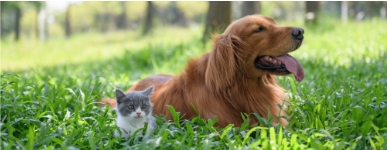
\includegraphics[height=2cm]{Segmentation.png} & 
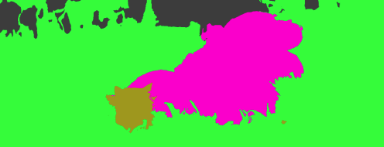
\includegraphics[height=2cm]{Segmentation-b.png} &
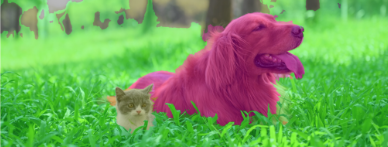
\includegraphics[height=2cm]{Segmentation-c.png}\\
(a) & (b) & (c)
\end{tabular}
\label{fig:segmentation}
{\small Fonte: \cite{minaee2020survey}}
\end{figure}


%\begin{figure}[h!]
%\centering
%\caption{\textcolor{red}{Exemplo de segmentação semântica. Em (a) temos três classes (Gato, Cachorro e Planta). A imagem (b) representa a máscara de segmentação separada por classe. Em (c) temos o retorno da imagem segmentada por classe.}}
%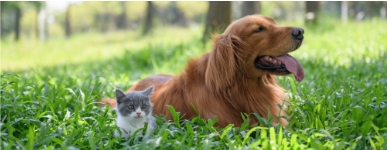
\includegraphics[width=1\textwidth]{Segmentation.png}
%\label{fig:segmentation}
%{\small Fonte:  \cite{minaee2020survey}}
%\end{figure}


\subsection{Classificação dos Algoritmos de Aprendizado de Máquina}

O algoritmo de aprendizado de máquina pode ser classificado em diferentes paradigmas de treinamento, dos quais se destacam o aprendizado supervisionado, não supervisionado, semi-supervisionado, por reforço e ativo.

No aprendizado supervisionado, o modelo recebe um conjunto de exemplos rotulados como dados de treinamento e aprende uma função que mapeia entradas para saídas desejadas. Após o treinamento, o modelo é capaz de realizar predições sobre exemplos não observados previamente. Este paradigma é amplamente uitilizado em tarefas como classificação, regressão e ranqueamento.

No aprendizado não supervisionado, o modelo tem acesso apenas a exemplos não rotulados e objetiva identificar estruturas, padrões latentes ou agrupamentos naturais presentes nos dados. Nesse contexto, a ausência de rótulos torna a avaliação quantitativa mais desafiadora. Problemas típicos incluem agrupamento (clustering), detecção de padrões, modelagem de densidade e redução de dimensionalidade.

No aprendizado semi-supervisionado, o modelo recebe um conjunto de treinamento composto simultaneamente por exemplos rotulados e não rotulados. Essa abordagem é adequada em cenários nos quais grandes volumes de dados não rotulados estão disponíveis, enquanto a rotulagem manual é custosa ou demorada. Tarefas como classificação, regressão e ranqueamento podem ser formuladas sob este paradigma. Assumindo que os dados não rotulados sigam a mesma distribuição que os dados rotulados, espera-se que sua exploração contribua para melhorar o desempenho em relação ao aprendizado supervisionado puro.

O Aprendizado por Reforço (\ac{RL}) constitui um subcampo da Inteligência Artificial (\ac{AI}) no qual um agente aprende a tomar decisões por meio da interação contínua com um ambiente, aprimorando progressivamente sua política de ação com base no \textit{feedback} recebido \cite{ghasemi2024comprehensive,li2022xrl}. Parte da literatura de seleção de amostras formula a escolha do que anotar como uma política aprendida por recompensa \cite{casanova2020reinforced,fang2017active}, o que o situa como alternativa ao Aprendizado Ativo discutido adiante.

Esse paradigma é mencionado aqui para completar a taxonomia e porque aparece em trabalhos relacionados, mas \textbf{não é empregado nesta dissertação}. A razão é a mesma que organiza o Capítulo \ref{cap_4}: aprender uma política de seleção por recompensa exige muitas rodadas de treinamento e avaliação para que o sinal de recompensa se acumule, e o regime estudado aqui tem três a cinco imagens anotadas e um modelo que se reestima por completo a cada anotação. Não há onde a política convergir.


%\begin{quote}

%\textbf{Aprendizado supervisionado:} O aprendiz recebe um conjunto de exemplos rotulados como dados de treinamento e realiza predições para todos os pontos não observados. Este é o cenário mais comum, associado a problemas de classificação, regressão e ranqueamento. O problema de detecção de spam, discutido na seção anterior, é um exemplo típico de aprendizado supervisionado.

%\textbf{Aprendizado não supervisionado:} O aprendiz recebe exclusivamente dados de treinamento não rotulados e realiza predições para pontos não vistos. Como, geralmente, não há exemplos rotulados disponíveis neste cenário, torna-se difícil avaliar quantitativamente o desempenho do aprendiz. Exemplos típicos de aprendizado não supervisionado incluem problemas de agrupamento (clustering) e redução de dimensionalidade.

%\textbf{Aprendizado semi-supervisionado:} O aprendiz recebe um conjunto de treinamento composto por dados rotulados e não rotulados, e realiza predições para pontos não observados. Essa abordagem é comum em contextos nos quais dados não rotulados são facilmente acessíveis, mas a rotulagem é cara ou trabalhosa. Diversos tipos de problemas, incluindo classificação, regressão e ranqueamento, podem ser enquadrados nesse paradigma. Espera-se que a distribuição dos dados não rotulados acessíveis possa auxiliar o aprendiz a alcançar um desempenho superior ao do aprendizado supervisionado puro.

%\end{quote}

%\begin{flushright}
%\footnotesize \cite{mohri2018foundations}
%\end{flushright}

\section{Aprendizado Ativo}
\label{sec_al_fund}

Diversas técnicas de \ac{ML} requerem grandes conjuntos de dados de treinamento para atingir seu desempenho ideal. Entretanto, o processo de anotação é frequentemente custoso, demorado e exige mão de obra especializada \cite{konyushkova2017learning}. 
No paradigma supervisionado, o algoritmo recebe um conjunto S composto por exemplos rotulados por especialistas, o que, em tarefas como segmentação de imagem, pode demandar horas de trabalho manual para rotular pixel a pixel. A partir desse conjunto, o modelo aprende uma função que mapeia os dados de entrada para as saídas desejadas.

%Para o processo de aprendizado de máquina supervisionado, o algoritmo recebe um dado $S$, rotulado por um especialista, muitas vezes demandando horas para que todos os pixels sejam rotulados. Ao receber esse conjunto de dados rotulado, o modelo aprenderá uma função que mapeia as entradas e produza a saída desejada. 

Durante o treinamento, o modelo processa pares $x_i,y_i$, em que $x_i$ representa a imagem original e $y_i$ a saída esperada.
Contudo, a exigência de um conjunto $S$ completamente rotulado torna o processo oneroso e pouco escalável. Nesse contexto, o aprendizado ativo \ac{AL} propõe estratégias para reduzir o custo de anotação por meio da seleção das amostras mais informativas para o treinamento \cite{settles2009active}. Dessa forma, em vez de rotular todo o conjunto de dados, o sistema seleciona iterativamente apenas os exemplos que proporcionam maior ganho esperado de desempenho, reduzindo substancialmente o esforço de anotação humana.

%Todavia, é necessário, durante esse processo, que haja um dado $S$ rotulado. Para reduzir o custo e o esforço envovlido na rotulagem, o Active Learning \ac{AL} propõe estratégias que selecionam os exemplos mais informativos e produtivos para anotação, otimizando o processo de treinamento e o custo para aquisição de modelos inteiramente rotulados \cite{settles2009active}.

\begin{figure}[h!]
\centering
\caption{Processo de funcionamento do ciclo de aprendizado ativo tradicional, destacando as etapas de treinamento inicial, seleção de amostras informativas, anotação pelo especialista e atualização incremental do modelo.}
%\caption{Processo de funcionamento do ciclo de aprendizado do modelo de Aprendizado Ativo}
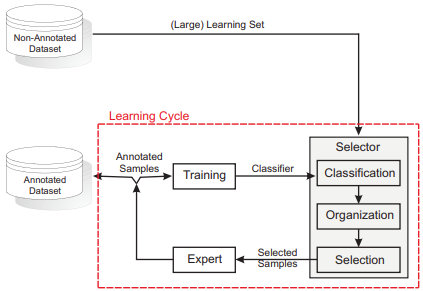
\includegraphics[width=10cm]{Active_Learning.png}
\label{fig:active_learning}\\
{\small Fonte: \cite{saito2014active}}
\end{figure}


De acordo com \citeonline{casanova2020reinforced}, os métodos de aprendizado ativo podem ser categorizados em dois grandes grupos: métodos baseados em estratégias projetadas manualmente e métodos orientados por dados.
Métodos baseados em estratégias projetadas manualmente agrupam abordagens que combinam heurísticas clássicas como incerteza, diversidade e representatividade \cite{konyushkova2017learning, bachman2017learning, konyushkova2018discovering, woodward2017active}. Já em métodos orientados por dados, o próprio modelo aprende quais amostras são mais informativas, utilizando o histórico de treinamento e estimadores internos de qualidade/amostragem \cite{konyushkova2017learning, bachman2017learning, konyushkova2018discovering, woodward2017active}.

A Tabela \ref{tab:active_learning_strategies} sintetiza e compara as principais estratégias de aprendizado ativo presentes na literatura. Nota-se que métodos guiados por incerteza, como a entropia, destacam-se no contexto de segmentação semântica, já que a maior concentração de incerteza ocorre tipicamente nas bordas dos objetos, regiões críticas que demandam maior atenção durante a correção manual dos rótulos.

%\textcolor{red}{A Tabela \ref{tab:active_learning_strategies} cria um comparativo entre as principais abordagens utilizadas.} 

%\textcolor{red}{Segundo a tabela \ref{tab:active_learning_strategies}, as abordagens baseadas em Incerteza (como a Entropia) são particularmente vantajosas para a segmentação semântica, pois a 'dúvida' do modelo geralmente se concentra nas bordas dos objetos, que é exatamente onde o refinamento humano é mais necessário.}


\begin{table}[h!]
\centering
\caption{Comparativo das principais estratégias de Active Learning.}
\label{tab:active_learning_strategies}
\resizebox{\textwidth}{!}{
\begin{tabular}{|p{2.5cm}|p{4.5cm}|p{4.5cm}|p{4.5cm}|p{3.5cm}|}
\hline
\textbf{Estratégia} & \textbf{Princípio de Seleção} & \textbf{Vantagens} & \textbf{Limitações} & \textbf{Exemplos}\\
\hline
\hline
\textbf{Baseada em Incerteza}\newline (Uncertainty-based) & 
Seleciona amostras com maior incerteza do modelo (alta entropia) & %em que o modelo tem a menor confiança na predição (maior entropia) & 
- Fácil de implementar\newline - Eficaz para refinar fronteiras de decisão (bordas na segmentação) & 
- Pode priorizar ruídos ou outliers\newline - Baixa diversidade das amostras selecionadas & 
- \ac{LC}\newline - \ac{ES}\newline - MC Dropout\\
\hline
\textbf{Baseada em Diversidade}\newline (Diversity-based) & 
Seleciona amostras que melhor representam a distribuição dos dados não rotulados & % (espalhamento) & 
- Reduz redundância\newline - Favorece cobertura de casos raros & %Evita redundância nos dados\newline - Garante cobertura de casos raros no conjunto de dados & 
- Alto custo computacional (clustering, distâncias no espaço latente) & %Custo computacional elevado (requer clustering ou cálculo de distâncias em todo o pool) & 
- Coreset\newline - $k$-Center-Greedy\newline - Clustering\\
\hline
\textbf{Mudança Esperada no Modelo}\newline \ac{EMC} & 
Seleciona amostras que potencialmente causariam maior impacto nos gradientes/perda & %Seleciona amostras que causariam a maior alteração nos gradientes ou na perda do modelo se fossem rotuladas & 
- Teoricamente a mais robusta, pois foca na melhoria direta do treino & 
- Muito lenta para \ac{DL} (exige simulações de treino) & %Extremamente lenta para Deep Learning (exige retreinos simulados ou cálculos pesados de gradiente) & 
- \ac{EGL}\\
\hline
\textbf{Híbrida}\newline (Hybrid) & 
Combina incerteza e diversidade para balancear informação e representatividade & %selecionar amostras informativas e representativas & 
- Equilibra exploration (diversidade) e exploitation (incerteza)\newline - Estado da arte atual & %Balanceia a exploração (diversidade) e a explotação (incerteza)\newline - Estado da arte atual & 
- Mais complexa de configurar (pesos e critérios combinados) & %Mais complexa de ajustar (hiperparâmetros de peso entre incerteza e diversidade) & 
- \ac{BADGE}\newline - \ac{VAAL}\\
\hline
\end{tabular}%
}
\fonte{Adaptado de \citeonline{ren2021survey}}
\end{table}



%\begin{itemize}
%\item Métodos que combinam diferentes estratégias de AL projetadas manualmentes (Roy \& McCallum, 2001; Osugi et al., 2005; Gal et al., 2017; Baram et al., 2004;
%Chu \& Lin, 2016; Hsu \& Lin, 2015; Ebert et al., 2012; Long \& Hua, 2015)

%\item Abordagens de AL orientadas por dados (Bachman et al., 2017; Fang et al., 2017; Konyushkova et al., 2017; Woodward \& Finn, 2016; Ravi \& Larochelle, 2018; Konyushkova et al., 2018) aprendem quais amostras são mais informativas para treinar um modelo usando informações do próprio modelo.
%\end{itemize}


%\subsubsection{Aprendizado por Reforço}

%Aprendizado por Reforço (Reinforcement Learning (\ac{RL})) é um subcampo da Inteligência Artificial (\ac{AI}), na qual um agente aprende a tomar decisões interagindo com o ambiente, potencializando a melhora do algoritmo de aprendizado \cite{ghasemi2024comprehensive}.

%Esse paradigma é inspirado nos mecanismos de aprendizado de tentativa e erro de humanos, onde o envolvimento com o ambiente serve como uma abordagem fundamental pra aprendizado sem um guia externo \cite{li2022xrl}.

%O trecho a seguir descreve formalmente como é o funcionamento do \ac{RL}.

%\begin{quote}
%Um agente de aprendizado por reforço (RL) interage com um ambiente ao longo do tempo. A cada instante de tempo \( t \), o agente recebe um estado \( s_t \) pertencente ao espaço de estados \( \mathcal{S} \), e seleciona uma ação \( a_t \) do espaço de ações \( \mathcal{A} \), seguindo uma política \( \pi(a_t|s_t) \), que representa o comportamento do agente, isto é, um mapeamento de estados \( s_t \) para ações \( a_t \).

%Em seguida, o agente recebe uma recompensa escalar \( r_t \) e transita para o próximo estado \( s_{t+1} \), de acordo com a dinâmica do ambiente (ou modelo), que é descrita pela função de recompensa \( R(s, a) \) e pela probabilidade de transição de estado \( P(s_{t+1}|s_t, a_t) \), respectivamente.

%Em problemas episódicos, esse processo continua até que o agente alcance um estado terminal, após o qual o episódio reinicia.

%O retorno \( R_t = \sum_{k=0}^{\infty} \gamma^k r_{t+k} \) é a soma acumulada das recompensas descontadas, onde \( \gamma \in (0, 1] \) é o fator de desconto.

%O objetivo do agente é maximizar a expectativa desse retorno de longo prazo a partir de cada estado.

%\end{quote}

%\begin{flushright}
%\footnotesize \cite{li2017drl}
%\end{flushright}

%Um dos paradigmas considerados um problema é como um agente interage com o ambiente para maximizar sua recompensa acumulada. A resposta pra esse problema é um processo conhecido como Processo de Decisão de Markov (\ac{MDP}) \cite{li2022xrl}

%O \ac{MDP} é um modelo de tomada de decisão sequencial no qual as transições de estado e recompensas dependem do estado atual e da ação tomada. Ele é formado um conjunto quíntuplo $(S, A, P, R, \gamma)$, onde:

%\begin{itemize}
%    \item $S$: Conjunto de estados
%    \item $A$: Conjunto de ações
%    \item $P$: Função de transição de estados
%    \item $R$: Função de recompensa
%    \item $\gamma$: Fator de desconto
%\end{itemize}

%O objetivo é encontrar uma política que maximize a recompensa acumulada esperada, chamada de retorno $G_t$. Para que isso ocorra, utiliza-se uma função $V_t(s)$, que estima o retorno esperado a partir do estado $s$, e $Q_a(s,a)$, que estima o retorno esperado a partir do estado $s$ quando tomada a ação $a$. \cite{ghasemi2024comprehensive}

\section{Superpixels}

Superpixels consistem na partição de uma imagem em regiões coesas formadas por pixels com características semelhantes, usualmente em termos de cor, textura e proximidade espacial, resultando em unidades elementares maiores e mais estruturadas do que pixels individuais. Essa representação reduz significativamente a redundância local e, por consequência, o volume de elementos a serem processados, o que contribui para acelerar etapas posteriores de segmentação e análise de imagens \cite{barcelos2024superpixel}. Nas últimas décadas, técnicas baseadas em superpixels têm recebido crescente atenção na literatura, especialmente devido ao seu potencial para reduzir o custo computacional e aumentar a eficiência em tarefas de segmentação semântica e instanciada \cite{vargas2014superpixel}.

A Figura \ref{fig:duas_figuras} ilustra um exemplo de imagem do conjunto de dados Cityscapes após etapas de processamento. Na Figura \ref{fig:duas_figuras}a, é apresentada a predição de segmentação semântica gerada pelo modelo \ac{SLIC}. Na Figura \ref{fig:duas_figuras}b tem-se a imagem particionada em unidades de superpixels adaptativos \cite{kim2023adaptive}, uma técnica de amostragem baseada em região (Region-Based Sampling) empregada no \ac{AL}. Nessa abordagem, os superpixels são utilizados como blocos elementares para identificar e selecionar regiões com maior incerteza preditiva (alta entropia), otimizando o processo de anotação ao direcionar o esforço humano apenas aos segmentos mais informativos para o treinamento subsequente. %Tal abordagem utiliza os superpixels como blocos elementares para calcular e amostrar regiões de maior incerteza preditiva (alta entropia), permitindo a otimização do processo de anotação ao focar o esforço humano apenas nos segmentos mais informativos para o treinamento subsequente.}

%Superpixel consiste em particionar imagens em regiões compostas por similiridade, criando pixels conectados. Isso ajuda a acelerar o processo de segmentação de imagem, reduzindo o trabalho que a máquina terá para processar informações redundantes  \cite{barcelos2024superpixel}
%Atualmente, superpixels tem recebido uma atenção especial para acelerar a segmentação de imagem \cite{vargas2014superpixel}.


\begin{figure}[h!]
\caption{Exemplo de imagens do conjunto de dados Cityscapes. (a)\textit{Ground-Truth} da imagem. (b) imagem particionada em superpixels}
\begin{tabular}{cc}
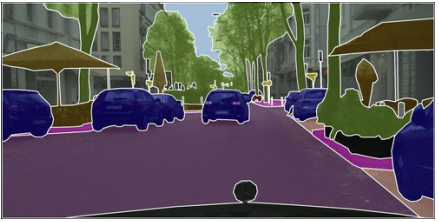
\includegraphics[height=3.75cm]{Oracle_Superpixel.PNG} &
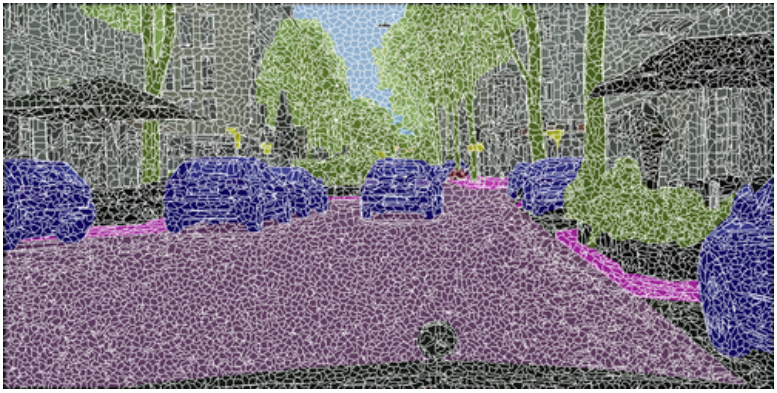
\includegraphics[height=3.75cm]{SuperPixel.PNG}\\
(a) & (b)
\end{tabular}
\label{fig:duas_figuras}
\centering
{\small Fonte: \cite{kim2023adaptive}}
\end{figure}


%\begin{figure}[h!]
%\centering
%\caption{Divisão da imagem em superpixels}
%\begin{minipage}[b]{0.45\textwidth}
%\centering
%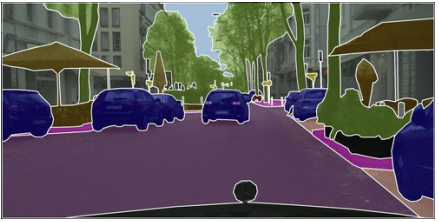
\includegraphics[width=\linewidth]{Oracle_Superpixel.PNG}
%\caption*{Imagem segmentada original}
%\label{fig:figura1}
%\end{minipage}
%\hfill
%\begin{minipage}[b]{0.45\textwidth}
%\centering
%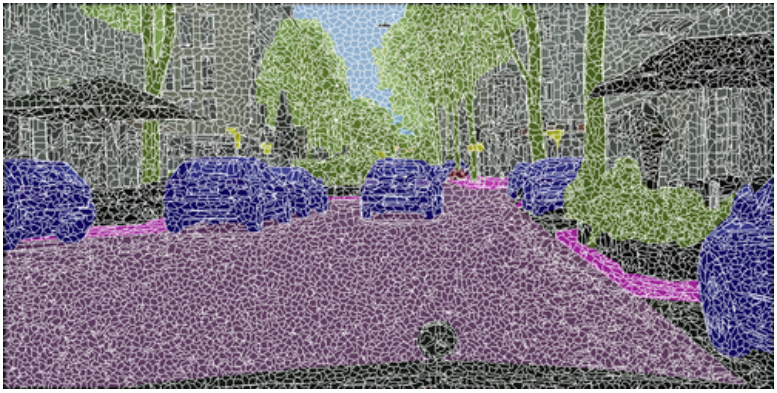
\includegraphics[width=\linewidth]{SuperPixel.PNG}
%\caption*{Imagem com superpixels}
%\label{fig:figura2}
%\end{minipage}
%\label{fig:duas_figuras}

%\vspace{0.3em}
%\centering
%{\small Fonte: \cite{kim2023adaptive}}
%\end{figure}



\section{Interactive Learning}

O aprendizado interativo (\ac{IL}) consiste em um paradigma de treinamento no qual o usuário participa ativamente do processo de anotação ou correção, selecionando objetos de interesse de forma precisa e incremental por meio de entradas simples, tais como cliques, pontos, scribbles ou delimitações por caixa (\textit{bounding boxes}) \cite{xu2016deep_arxiv}.
A interação humana pode ser empregada tanto para orientar a segmentação de objetos específicos, quanto para refinar predições previamente geradas pelo modelo, corrigindo regiões mal segmentadas ou omitidas.

%O Aprendizado interativo (\ac{IL}) é o aprendizado que permite os usuários selecionarem os objetos de interesse precisavemente e interativamente provendo entradas como pontos ou seleções de caixa \cite{xu2016deep_arxiv}. 

O objetivo central da segmentação de imagens interativa é aproximar-se, com a maior fidelidade possível, da máscara de referência, utilizando o menor número de interações humanas, comumente mensuradas em número de cliques \cite{sofiiuk2020fbrs_arxiv}. Em geral, os sistemas oferecem uma interface na qual o usuário pode iterativamente adicionar cliques positivos e negativos até que o resultado atinja o nível de precisão desejado.
De modo geral, a literatura reporta duas direções complementares no uso de IL: (i) abordagens que empregam o sinal interativo como mecanismo de refinamento incremental do modelo de segmentação; e (ii) abordagens que utilizam a interação para guiar a segmentação de objetos específicos ou para corrigir inconsistências localizadas nas máscaras produzidas automaticamente.

A Figura \ref{fig:figura1} ilustra o fluxo de interação humano-computador no contexto da segmentação interativa. A imagem é apresentada ao usuário especialista por meio de uma interface gráfica, na qual ele fornece cliques de feedback para orientar o processo de refinamento. O botão esquerdo do mouse é utilizado para inserir \textit{foreground clicks} (pontos positivos), enquanto o botão direito registra \textit{background clicks} (pontos negativos), permitindo corrigir falhas na predição ou remover áreas indevidamente segmentadas. Esses cliques são interpretados pelo modelo como restrições rígidas (\textit{hard constraints}). Após cada iteração de processamento, o modelo retorna uma máscara de segmentação atualizada. Esse ciclo interativo se repete até que a segmentação atinja o nível de precisão desejado pelo especialista, caracterizando uma abordagem de aprendizado interativo (Interactive Learning).

%\textcolor{red}{A Figura \ref{fig:figura1} ilustra o fluxo de interação humano-computador no contexto da segmentação interativa. A imagem é apresentada ao usuário especialista por meio de uma interface gráfica para o fornecimento de cliques de feedback. O usuário utiliza o botão esquerdo para indicar os foreground clicks (pontos positivos) e o botão direito para fornecer os background clicks (pontos negativos), corrigindo falhas na predição ou áreas indesejadas. Esses inputs são interpretados pelo modelo como restrições (hard constraints). Após o processamento, o modelo retorna a máscara de segmentação refinada. O ciclo de refinamento iterativo é repetido até que a segmentação atinja a precisão desejada pelo especialista, caracterizando uma abordagem de aprendizado interativo (Interactive Learning).}

%A seleção de objetos de interesse através de demarcações utilizando especialistas pode ser utilizada tanto para a segmentação de objetos específicos, quanto para melhora e refinamento de segmentações que o modelo possa ter apresentado de forma errada.


\begin{figure}[h!]
\centering
\caption{Exemplo ilustrativo de interface interativa. 
(a) Imagem com cliques do usuário: pontos verdes representam regiões do objeto de interesse e pontos vermelhos indicam regiões de fundo.
(b) Mapa de probabilidades gerado pelo modelo.
(c) Resultado final da segmentação do cachorro.}
\label{fig:figura1}

\begin{minipage}{0.32\linewidth}
    \centering
    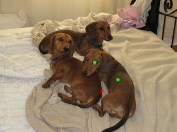
\includegraphics[width=\linewidth]{interactive_example_a.png}\\
    (a)
\end{minipage}
\hfill
\begin{minipage}{0.32\linewidth}
    \centering
    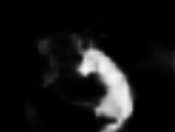
\includegraphics[width=\linewidth]{interactive_example_b.png}\\
    (b)
\end{minipage}
\hfill
\begin{minipage}{0.32\linewidth}
    \centering
    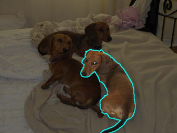
\includegraphics[width=\linewidth]{interactive_example_c.png}\\
    (c)
\end{minipage}

\vspace{0.2cm}
{\small Fonte: \cite{xu2016deep_arxiv}}
\end{figure}


%O objetivo da segmentação de imagem interativa é obter uma acurácia próxima a da máscara do objeto usando o menos cliques possível do usuário. A maior parte dos métodos possui uma inferface onde o usuário pode realizar cliques positivos e cliques negativos diversas vezes, até que a máscara do objeto desejada seja obtida. \cite{sofiiuk2020fbrs_arxiv}

%Algumas abordagens utilizam o interactive learning para auxiliar no refinamento do modelo de segmentação, outros, utilizam para que o usuário escolha o objeto a ser segmentado, ou que para faça a correção pontual na segmentação da imagem gerada.



\section{Continual Learning}\label{sec_cl}

O aprendizado contínuo (\ac{CL}) constitui um subcampo da Inteligência Artificial dedicado ao desenvolvimento de modelos capazes de aprender de forma sequencial e incremental a partir de fluxos contínuos de dados, sem a necessidade de serem completamente retreinados a cada novo conjunto de informações. Essa habilidade de acumular conhecimento ao longo do tempo, característica intrínseca à inteligência biológica, permanece um desafio central para redes neurais artificiais \cite{delange2021continual}.

O principal obstáculo associado à \ac{CL} é o fenômeno conhecido como esquecimento catastrófico (catastrophic forgetting), no qual a atualização dos parâmetros do modelo para incorporar novos conhecimentos interfere negativamente no desempenho obtido em tarefas previamente aprendidas.

Diversos métodos têm sido propostos na literatura para mitigar esse problema. Entre eles, destacam-se três classes predominantes:

\begin{enumerate}

\item \textbf{Métodos baseados em regularização}: introduzem termos adicionais (penalidades) na função de perda com a finalidade de restringir alterações em parâmetros que foram identificados como essenciais para tarefas anteriores. Um exemplo notável dessa categoria é o \ac{EWC}, que estima a importância dos pesos e penaliza alterações proporcionais a essa relevância \cite{kirkpatrick2017overcoming}.

\item \textbf{Métodos baseados em replay}: consistem em preservar um subconjunto reduzido dos dados de tarefas passadas e reexibi-los ao modelo durante o treinamento de novas tarefas, evitando que antigos conhecimentos sejam sobrescritos. O método iCaRL, por exemplo, emprega conjuntos representativos de exemplares para reter desempenho histórico ao longo das iterações de aprendizagem \cite{rebuffi2017icarl}.

\item \textbf{Métodos baseados em Destilação de Conhecimento}: introduzidos inicialmente por \cite{hinton2015distilling}, tratam o processo de transferência de conhecimento de um modelo para outro de forma análoga à relação professor-aluno. A estratégia consiste em induzir o modelo aluno a imitar não apenas as decisões finais do modelo professor, mas também sua distribuição de probabilidades, preservando informações relevantes mesmo diante de novos dados.
\end{enumerate}

As três abordagens compartilham um pressuposto: existe um otimizador que desloca pesos, e é sobre esse deslocamento que elas atuam. A regularização penaliza a mudança dos pesos importantes, o ensaio reapresenta dados antigos ao otimizador, e a destilação faz o modelo aluno imitar as saídas do professor. \textbf{Nenhuma dessas operações está definida para o \ac{FLIM}}, que não possui função de perda nem otimizador.

Este trabalho não adota, portanto, nenhuma das três. O mecanismo investigado no Capítulo~\ref{cap_3} atua sobre o objeto que de fato se desloca no \ac{FLIM}: o banco de filtros, reestimado por agrupamento a cada nova anotação. A Seção~\ref{sec_lacuna} retoma esse ponto como a lacuna específica que a dissertação endereça.

%A Aprendizagem Contínua (\ac{CL}) é uma subárea da inteligência artificial que visa desenvolver modelos capazes de aprender de forma sequencial e incremental a partir de um fluxo contínuo de dados, sem a necessidade de serem retreinados do zero. Esta capacidade de acumular conhecimento ao longo do tempo é uma característica fundamental da inteligência biológica, mas representa um desafio significativo para as redes neurais artificiais \cite{delange2021continual}.

%Um dos principais obstáculos a ser superado é o chamado esquecimento carastrófico (catastrophic forgetting), onde o ajuste dos pesos do modelo ao aprender uma nova tarefa, interfere com o conhecimento que o modelo adquiriu anteriormente, alterando a performance em tarefas antigas.

%Para mitigar esse problema, foram propostas diversas abordagens, dentre elas, três se destacam: 

%\begin{enumerate}
%\item Abordagens baseadas em regularização: essa abordagem adiciona uma penalidade na função de perda, o que evita a atualização dos pesos considerados importantes para as tarefas antigas. A estratégia mais proeminente aqui é a Abordagem de Consolidação Elástica de Pesos, na qual calcula a importância de cada peso e penaliza a sua modificação \cite{kirkpatrick2017overcoming}
%\item A segunda abordagem consiste em estratégias de replay: Armazena pequenos subconjunto de dados de tarefas antigas, apresentando ao modelo durante o treinamento de novas tarefas. Um dos exemplos dessa abordagem é o iCaRL, que utiliza exemplo de dados antigos para retreinar o modelo a cada nova etapa do conhecimento \cite{rebuffi2017icarl}.
%\item A terceira abordagem é a Destilação de Conhecimento: esse método foi criado por \cite{hinton2015distilling}, como um modelo de passagem de conhecimento analogo a um professor e um aluno. A ideia é que o aluno aprenda a imitar as saídas do professor, não apenas as respostas finais, mas a distribuição de probabilidade completa.
%\end{enumerate}

%No presente trabalho, é adotada a abordagem de Destilação de Conhecimento.


\section{Feature Learning from Image Markers}

As redes convolucionais descritas até aqui ajustam seus filtros por retropropagação, o que exige grandes conjuntos anotados e capacidade computacional proporcional. O \ac{FLIM}, proposto por \cite{souza2020flim}, parte de uma premissa diferente: os filtros não são descobertos por otimização, e sim estimados a partir de marcadores que o especialista desenha sobre poucas imagens representativas.

O procedimento é estimar os filtros camada a camada. Para cada marcador, o método recorta os patches centrados nos pixels marcados, agrupa esses patches e usa os centróides resultantes como filtros daquela camada. A saída da camada serve de entrada para o mesmo procedimento na camada seguinte, de modo que a estimação avança sem nenhum passo de retropropagação e sem inicialização aleatória de pesos. Com isso, o especialista deixa de fornecer apenas rótulos e passa a indicar quais regiões da imagem discriminam o objeto.

A consequência prática é a redução drástica do número de imagens anotadas. Enquanto uma rede treinada por retropropagação costuma exigir milhares de exemplos, redes \ac{FLIM} são construídas a partir de uma a poucas imagens por classe \cite{benato2020cnnmarkers}. O método foi aplicado a delineamento de objetos \cite{souza2020flim} e a classificação de imagens de sensoriamento remoto \cite{souza2020coconut}, com resultados comparáveis e às vezes superiores aos da mesma arquitetura treinada do zero.

\subsection{Decodificadores adaptativos}

Um encoder \ac{FLIM} produz mapas de ativação, não uma máscara de segmentação. É preciso então converter esses mapas em uma decisão por pixel. \cite{soares2026flim} propõem decodificadores adaptativos para essa conversão: em vez de aprender um decodificador fixo, os pesos são calculados para cada imagem de entrada por uma função heurística que estima se cada canal de ativação responde ao objeto ou ao fundo.

Essa escolha mantém a rede leve, porque o decodificador é uma convolução ponto a ponto com pesos em $\{-1, +1\}$, e preserva a propriedade central do \ac{FLIM}: nenhum parâmetro é ajustado por gradiente. O trabalho relata redes centenas de vezes menores que modelos considerados leves, treinadas com três a quatro imagens representativas. Trabalhos subsequentes na mesma linha exploram kernels separáveis dilatados para reduzir ainda mais o número de parâmetros \cite{joao2025flyweight}.

É esse arranjo, encoder \ac{FLIM} com decodificador adaptativo, que o presente trabalho reproduz e sobre o qual aplica as estratégias de aprendizado ativo, interativo e contínuo descritas nas seções anteriores. A Figura~\ref{fig_flim_cap2} mostra o arranjo completo aplicado a uma imagem, da entrada ao erro por pixel.

\begin{figure}[htb]
\centering
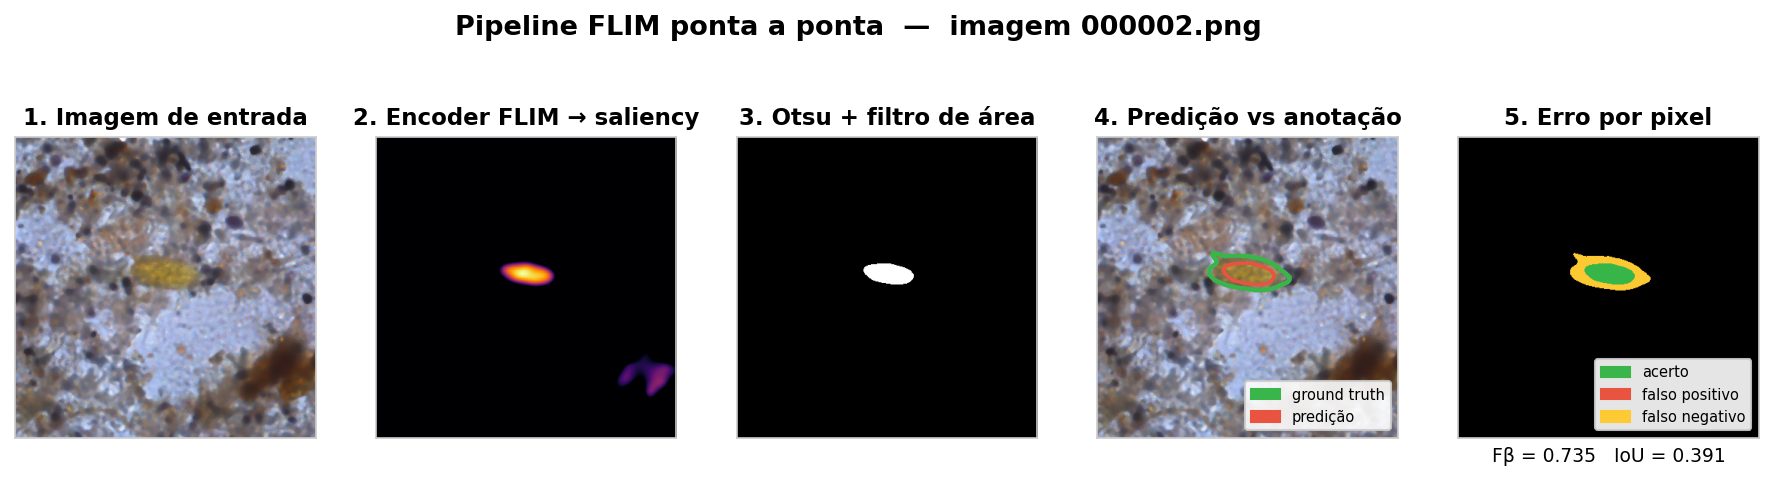
\includegraphics[width=\linewidth]{flim_pipeline.png}
\caption[O arranjo \acs{FLIM} com decodificador adaptativo]{O arranjo aplicado a uma imagem de microscopia. O codificador \ac{FLIM}, cujos filtros são centróides de agrupamentos sobre os trechos marcados, produz o mapa de saliência; o decodificador adaptativo e o pós-processamento produzem a máscara; a comparação com a anotação de referência dá as métricas. Nenhum parâmetro do percurso foi ajustado por gradiente.}
\label{fig_flim_cap2}
\end{figure}

\subsection{Por que a combinação com AL e CL não é imediata}

As três estratégias discutidas neste capítulo pressupõem, de formas diferentes, um modelo treinado por gradiente.

O \ac{AL} supõe que o modelo melhora de maneira previsível quando recebe rótulos adicionais, e por isso faz sentido escolher quais exemplos rotular. O \ac{CL} supõe que o esquecimento catastrófico decorre do deslocamento dos pesos durante o ajuste por gradiente, e as três classes de método descritas na Seção \ref{sec_cl} combatem exatamente esse deslocamento: regularização penaliza a mudança de pesos importantes, replay reapresenta dados antigos ao otimizador, e destilação faz o modelo aluno imitar as saídas do professor. Nenhuma dessas operações está definida para um modelo sem otimizador.

No \ac{FLIM} a relação entre anotação e parâmetros é de outra natureza. Os filtros são centróides de agrupamentos sobre os patches marcados, e o banco de filtros é compartilhado por todas as imagens, inclusive as não anotadas. Acrescentar marcadores altera o conjunto de patches candidatos, o que altera o agrupamento e, por consequência, os filtros já estimados. A anotação adicional, portanto, não refina o modelo de forma incremental: ela reestima o extrator de atributos.

Essa diferença é o ponto de partida da metodologia apresentada no Capítulo \ref{cap_3}, e a sua caracterização quantitativa é o objeto dos experimentos relatados no Capítulo \ref{cap_4}.


\section{Trabalhos Relacionados}

Conforme discutido anteriormente (Seção \ref{cap_1}), a literatura apresenta uma ampla variedade de estratégias e métodos voltados à potencialização de modelos de Inteligência Artificial, buscando equilibrar custo computacional, tempo de treinamento e desempenho preditivo. Em linhas gerais, os estudos diferenciam-se pelas abordagens adotadas para mitigar limitações recorrentes, tais como o tempo elevado de processamento, escassez de dados anotados, necessidade de maior acurácia e a integração de mecanismos avançados de aprendizagem, incluindo \ac{AL}, \ac{CL}, \ac{IL}, arquiteturas híbridas, novos algoritmos, introdução de adaptadores, otimizações em transformers, entre outros.
%Nesse contexto, é apresentada a Tabela \ref{tab:trabalhos_relacionados} com os principais trabalhos relacionados, organizada de modo a caracterizar cada proposta quanto à sua abordagem central, bem como destacar suas principais vantagens e limitações.

%Conforme visto anteriormente (Seção 1), há diversas estratégias e métodos para que um modelo de Inteligência Artificial seja potencializado, equilibrando métricas de custo computacional e tempo gasto. Em geral, os trabalhos destacam-se pelas diferentes abordagens afim de melhorar as lacunas existentes, como a demora de execução de um modelo, falta de dados, melhorias de acurácia e aplicações de métodos diversos, como \ac{AL}, \ac{CL}, \ac{IL}, mistura de abordagens, novos algoritmos, adaptadores, melhorias nos transformers, entre outros. A seguir, apresenta-se uma tabela dos principais trabalhos relacionados, caracterizando-os conforme sua abordagem, vantagens e desvantagens de cada um. 

% \begin{table}[h!]
% \centering
% \caption{Trabalhos relacionados à segmentação de imagens.}
% \label{tab:trabalhos_relacionados}
% \tiny
% \begin{adjustbox}{angle=90}
% \begin{tabular}{|c|l|l|l|l|c|c|}
% \hline
% \textbf{Nº} & \textbf{Autores} & \textbf{Técnica Principal} & \textbf{Algoritmo/Modelo} & \textbf{Dataset(s)} & \textbf{AL} & \textbf{VLM} \\\hline
% 1 & \cite{stutz2018superpixels} & Survey (Superpixels) & Taxonomia de superpixels & BSDS500, NYUV2, SUNRGBD & - & - \\\hline
% 2 & \cite{hesamian2020medical} & Survey (Medicina) & Revisão DL médica & - & - & - \\\hline
% 3 & \cite{jha2020kvasirseg} & Arquitetura CNN & U-Net, variantes & Kvasir-SEG & - & - \\\hline
% 4 & \cite{emara2019liteseg} & Arquitetura CNN (Leve) & LiteSeg (ASPP, depthwise) & Cityscapes & - & - \\\hline
% 5 & \cite{zhang2023attention} & Arquitetura CNN (Atenção) & SE-ASPP & Cityscapes, CamVid & - & - \\\hline
% 6 & \cite{wang2021boundary} & Estratégia (Função de Perda) & Boundary Loss & Cityscapes & - & - \\\hline
% 7 & \cite{liao2023dual} & Estratégia (Label Noise) & Dual-task Crowd Labels & Cityscapes, CamVid & - & - \\\hline
% 8 & \cite{gansbeke2021unsupervised} & Estratégia (Aprend. Contrastiva) & Object Mask Contrast & Cityscapes, \ac{PascalPascalVOC2012}& - & - \\\hline
% 9 & \cite{yang2018curriculum} & Estratégia (Adaptação de Domínio) & Curriculum Adaptation & Cityscapes & - & - \\\hline
% 10 & \cite{hoffman2016unsupervised} & Estratégia (Adaptação de Domínio) & Adversarial Training & Cityscapes & - & - \\\hline
% 11 & \cite{zhang2019spda} & Estratégia (Aumento c/ Superpixel) & \ac{SLIC} + U-Net & BraTS, Nuclei, LiTS, CVC-ClinicDB & - & - \\\hline
% 12 & \cite{franchi2021robust} & Estratégia (Aumento c/ Superpixel) & DeepLabv3+ & Cityscapes & - & - \\\hline
% 13 & \cite{zhang2020dualwindow} & Estratégia (Aumento c/ Superpixel) & Dual-Window Aug. & PaviaU, Salinas & - & - \\\hline
% 14 & \cite{delarosa2022improving} & Estratégia (Aumento Sintético) & DeepLab V2, Xception & Cityscapes & - & - \\\hline
% 15 & \cite{baranchuk2021label} & Estratégia (Semi-supervisão) & DDPMs + seg. & Cityscapes & - & - \\\hline
% 16 & \cite{wang2020solo} & Técnica (Seg. de Instância) & SOLO & - & - & - \\\hline
% 17 & \cite{han2020dvsnet} & Técnica (Seg. de Vídeo) & DVSNet (Path decision) & Cityscapes & - & - \\\hline
% 18 & \cite{wu2023medical} & VLM (Adaptação c/ Adapter) & Medical SAM Adapter & PIPO-FAN, REFUGE2, ISIC, etc. & - & \checkmark \\\hline
% 19 & \cite{huang2024adapting} & VLM (Adaptação c/ Adapter) & Residual adapters & BrainMRI, LiverCT, RESC & - & \checkmark \\\hline
% 20 & \cite{gowda2024ccsam} & VLM (Fusão CNN+VLM) & CC-SAM (CNN + SAM) & TN3K, DDTI, TG3K, BUSI, etc. & - & \checkmark \\\hline
% 21 & \cite{koleilat2024medclipsamv2} & VLM (Fusão Multimodal) & MedCLIP-SAMv2 & ROCO, MedPix, BUSI, etc. & - & \checkmark \\\hline
% 22 & \cite{liu2024grounded} & VLM (Fusão Open-World) & SAM + Grounding DINO & COCO, LVIS, ADE20K, VG & - & \checkmark \\\hline
% 23 & \cite{xie2022ripu} & AL (Estratégia: Incerteza) & RIPU & Cityscapes & \checkmark & - \\\hline
% 24 & \cite{zheng2024alintro} & AL (Estratégia: Incerteza) & AL-Intro (SOD) & NJU2K, NLPR, SIP, STERE & \checkmark & - \\\hline
% 25 & \cite{konyushkova2017learning} & AL (Estratégia: Meta-Learning) & Meta-AL strategy & USPS, MNIST, BioID & \checkmark & - \\\hline
% 26 & \cite{kim2023adaptive} & AL (Estratégia: Baseada em Região) & Adaptive Superpixel (MCLU) & Cityscapes, \ac{PascalPascalVOC2012}& \checkmark & - \\\hline
% 27 & \cite{mackowiak2018cereals} & AL (Estratégia: Baseada em Região) & CEREALS (superpixels) & Cityscapes & \checkmark & - \\\hline
% 28 & \cite{rangnekar2022region} & AL (Estratégia: Baseada em Região) & Teacher-Student & Cityscapes, CamVid & \checkmark & - \\\hline
% 29 & \cite{franco2023halo} & AL (Estratégia: Otimização HW) & HALO & Cityscapes (GTAV sintético) & \checkmark & - \\\hline
% 30 & \cite{casanova2020reinforced} & AL (Híbrido: AL + RL) & DQN (seleção de regiões) & Cityscapes, CamVid & \checkmark & - \\\hline
% 31 & \cite{rangnekar2022mean} & AL (Híbrido: AL + Semi-sup.) & Mean Teacher + Contrastive & Cityscapes, CamVid & \checkmark & - \\\hline
% 32 & \cite{karamcheti2021dial} & AL (Híbrido: AL + IL) & DIAL (Bayesiana) & ISPRS Vaihingen, \ac{PascalVOC2012}& \checkmark & - \\\hline
% 33 & \cite{triebel2014active} & AL (Híbrido: AL + IL Online) & Sparse GPs & GrabCut & \checkmark & - \\\hline
% 34 & \cite{vu2023active} & AL (Híbrido: AL + CL) & CL + Acquisition Function & ASC + 20News & \checkmark & - \\\hline
% 35 & \cite{zheng2021continual} & CL (Híbrido: CL + IL) & Continual + Uncertainty & ISIC, CHAOS, \ac{PascalVOC2012}& \checkmark & - \\\hline
% \end{tabular}
% \end{adjustbox}
% \end{table}

\begin{table}[h!]
\centering
\caption{Trabalhos relacionados à segmentação de imagens}% com colunas adicionais para IL e CL.}
\label{tab:trabalhos_relacionados}
\tiny
\begin{adjustbox}{angle=90, max height=\textheight}
\begin{tabular}{|c|l|l|l|l|c|c|c|c|}
\hline
\textbf{Nº} & \textbf{Autores} & \textbf{Técnica Principal} & \textbf{Algoritmo/Modelo} & \textbf{Dataset(s)} & \textbf{AL} & \textbf{VLM} & \textbf{IL} & \textbf{CL} \\\hline

1 & \cite{stutz2018superpixels} & Survey (Superpixels) & Taxonomia de superpixels & BSDS500, NYUV2, SUNRGBD & - & - & - & - \\\hline
2 & \cite{hesamian2020medical} & Survey (Medicina) & Revisão DL médica & - & - & - & - & - \\\hline
3 & \cite{jha2020kvasirseg} & Arquitetura CNN & U-Net, variantes & Kvasir-SEG & - & - & - & - \\\hline
4 & \cite{emara2019liteseg} & Arquitetura CNN (Leve) & LiteSeg (ASPP, depthwise) & Cityscapes & - & - & - & - \\\hline
5 & \cite{zhang2023attention} & Arquitetura CNN (Atenção) & SE-ASPP & Cityscapes, CamVid & - & - & - & - \\\hline
6 & \cite{wang2021boundary} & Estratégia (Função de Perda) & Boundary Loss & Cityscapes & - & - & - & - \\\hline
7 & \cite{liao2023dual} & Estratégia (Label Noise) & Dual-task Crowd Labels & Cityscapes, CamVid & - & - & - & - \\\hline
8 & \cite{gansbeke2021unsupervised} & Estratégia (Aprend. Contrastiva) & Object Mask Contrast & Cityscapes, \ac{PascalVOC2012}& - & - & - & - \\\hline
9 & \cite{yang2018curriculum} & Estratégia (Adaptação de Domínio) & Curriculum Adaptation & Cityscapes & - & - & - & - \\\hline
10 & \cite{hoffman2016unsupervised} & Estratégia (Adaptação de Domínio) & Adversarial Training & Cityscapes & - & - & - & - \\\hline
11 & \cite{zhang2019spda} & Estratégia (Aumento c/ Superpixel) & \ac{SLIC} + U-Net & BraTS, Nuclei, LiTS, CVC-ClinicDB & - & - & - & - \\\hline
12 & \cite{franchi2021robust} & Estratégia (Aumento c/ Superpixel) & DeepLabv3+ & Cityscapes & - & - & - & - \\\hline
13 & \cite{zhang2020dualwindow} & Estratégia (Aumento c/ Superpixel) & Dual-Window Aug. & PaviaU, Salinas & - & - & - & - \\\hline
14 & \cite{delarosa2022improving} & Estratégia (Aumento Sintético) & DeepLab V2, Xception & Cityscapes & - & - & - & - \\\hline
15 & \cite{baranchuk2021label} & Estratégia (Semi-supervisão) & DDPMs + seg. & Cityscapes & - & - & - & - \\\hline
16 & \cite{wang2020solo} & Técnica (Seg. de Instância) & SOLO & - & - & - & - & - \\\hline
17 & \cite{han2020dvsnet} & Técnica (Seg. de Vídeo) & DVSNet (Path decision) & Cityscapes & - & - & - & - \\\hline
18 & \cite{wu2023medical} & VLM (Adaptação c/ Adapter) & Medical SAM Adapter & PIPO-FAN, REFUGE2, ISIC, etc. & - & \checkmark & - & - \\\hline
19 & \cite{huang2024adapting} & VLM (Adaptação c/ Adapter) & Residual adapters & BrainMRI, LiverCT, RESC & - & \checkmark & - & - \\\hline
20 & \cite{gowda2024ccsam} & VLM (Fusão CNN+VLM) & CC-SAM & TN3K, DDTI, TG3K, BUSI, etc. & - & \checkmark & - & - \\\hline
21 & \cite{koleilat2024medclipsamv2} & VLM (Fusão Multimodal) & MedCLIP-SAMv2 & ROCO, MedPix, BUSI, etc. & - & \checkmark & - & - \\\hline
22 & \cite{liu2024grounded} & VLM (Fusão Open-World) & SAM + Grounding DINO & COCO, LVIS, ADE20K, VG & - & \checkmark & - & - \\\hline
23 & \cite{xie2022ripu} & AL (Estratégia: Incerteza) & RIPU & Cityscapes & \checkmark & - & - & - \\\hline
24 & \cite{zheng2024alintro} & AL (Estratégia: Incerteza) & AL-Intro (SOD) & NJU2K, NLPR, SIP, STERE & \checkmark & - & - & - \\\hline
25 & \cite{konyushkova2017learning} & AL (Meta-Learning) & Meta-AL strategy & USPS, MNIST, BioID & \checkmark & - & - & - \\\hline
26 & \cite{kim2023adaptive} & AL (Região) & Adaptive Superpixel (MCLU) & Cityscapes, \ac{PascalVOC2012}& \checkmark & - & - & - \\\hline
27 & \cite{mackowiak2018cereals} & AL (Região) & CEREALS (superpixels) & Cityscapes & \checkmark & - & - & - \\\hline
28 & \cite{rangnekar2022region} & AL (Região) & Teacher-Student & Cityscapes, CamVid & \checkmark & - & - & - \\\hline
29 & \cite{franco2023halo} & AL (Otimização HW) & HALO & Cityscapes (GTAV sintético) & \checkmark & - & - & - \\\hline
30 & \cite{casanova2020reinforced} & AL + RL & DQN (seleção de regiões) & Cityscapes, CamVid & \checkmark & - & - & - \\\hline
31 & \cite{rangnekar2022mean} & AL + Semi-Sup. & Mean Teacher + Contrastive & Cityscapes, CamVid & \checkmark & - & - & - \\\hline
32 & \cite{karamcheti2021dial} & AL + IL & DIAL (Bayesiana) & ISPRS Vaihingen, \ac{PascalVOC2012}& \checkmark & - & \checkmark & - \\\hline
33 & \cite{triebel2014active} & AL + IL Online & Sparse GPs & GrabCut & \checkmark & - & \checkmark & - \\\hline
34 & \cite{vu2023active} & AL + CL & CL + Acquisition Function & ASC + 20News & \checkmark & - & - & \checkmark \\\hline
35 & \cite{zheng2021continual} & CL + IL & Continual + Uncertainty & ISIC, CHAOS, \ac{PascalVOC2012}& - & - & \checkmark & \checkmark \\\hline
\end{tabular}
\end{adjustbox}
\end{table}


\begin{table}[h!]
\centering
\caption{Síntese dos principais datasets públicos reportados na literatura e utilizados como referência para treinamento e avaliação em segmentação semântica.}
\label{tab:datasets}
\tiny
\begin{adjustbox}{angle=90}
\begin{tabular}{|c|l|l|l|l|c|c|c|}
\hline
\textbf{Nº} & \textbf{Nome} & \textbf{Tamanho} & \textbf{Número de imagens} & \textbf{Resolução} & \textbf{Número de classes} & \textbf{Tipo de imagens} & \textbf{Ano} \\ \hline

1 & \ac{PascalVOC2012} & 4 GB & 11.530 (treino/val) & 500x375 & 20 & Segmentação de Objetos & 2012 \\ \hline
2 & Cityscapes & 25 GB & 5.000  & 2048x1024 & 30 & Cenas Urbanas & 2016 \\ \hline
3 & CamVid & 570 MB & 701 frames & 960x720 & 32 & Cenas Urbanas (Vídeo) & 2008 \\ \hline
4 & COCO & 50 GB & 330.000 & Variável & 80 & Segmentação de Objetos & 2014 \\ \hline
5 & LVIS & 25 GB & 164.000 & Variável & 1.203 & Segmentação de Instâncias & 2019 \\ \hline
6 & ADE20K & 3 GB & 27.000 & Variável & 150 & Análise de Cenas & 2016 \\ \hline
7 & GTA V (Sintético) & 180 GB & 25.000 & 1914x1052 & 19 & Cenas Urbanas (Sintético) & 2016 \\ \hline
8 & NYU Depth V2 & 5.5 GB & 1.449 & 640x480 & 40 & Cenas Internas (RGB-D) & 2012 \\ \hline
9 & SUN RGB-D & 60 GB & 10.335 & Variável & 37 & Cenas Internas (RGB-D) & 2015 \\ \hline
10 & NLPR & ~1 GB & 1.000 pares & 640x480 & 1 & Detecção de Obj. Salientes & 2014 \\ \hline
11 & NJU2K & 1.5 GB & 1.985 pares & Variável & 1 & Detecção de Objetos & 2014 \\ \hline
12 & STERE & 100 MB & 1.000 pares & 1024x768 & 1 & Detecção de Objetos (Estéreo) & 2015 \\ \hline
13 & Kvasir-SEG & 2 GB & 1.000 & 576x720 & 1 & Médica (Pólipo Colorretal) & 2020 \\ \hline
14 & BraTS & 200 GB & ~3.000 (3D) & 240x240x155 & 3 & Médica 3D (Tumor Cerebral) & 2012 \\ \hline
15 & LiTS / LiverCT & 80 GB & 131 scans CT & 512x512xZ & 2 & Médica 3D (Fígado) & 2017 \\ \hline
16 & CVC-ClinicDB & 50 MB & 612 & 384x288 & 1 & Médica (Endoscopia) & 2015 \\ \hline
17 & REFUGE2 & 3.8 GB & 1.200 & UHD (várias) & 2 & Médica (Oftalmologia) & 2020 \\ \hline
18 & ISIC & Variável & > 203.000 & Variável & 2-7 & Médica (Dermatologia) & 2016 \\ \hline
19 & BrainMRI & 350 MB & 3.929 & 256x256 & 1 & Médica (Tumor Cerebral) & 2020 \\ \hline
20 & RESC & 500 MB & 110 scans & Variável & 3 & Médica (Edema Retinal) & 2018 \\ \hline
21 & TN3K & 200 MB & 3.500 & 400x400 & 1 & Médica (Nódulo Tireoide) & 2022 \\ \hline
22 & DDTI & 1.5 GB & 5.000 & Variável & 1 & Médica (Raio-X Panorâmico) & 2022 \\ \hline
23 & TG3K & 250 MB & 3.100 & 400x400 & 1 & Médica (Glândula Tireoide) & 2022 \\ \hline
24 & BUSI & 250 MB & 780 & ~500x500 & 3 & Médica (Ultrassom de Mama) & 2019 \\ \hline
25 & CHAOS & 20 GB & 80 scans & 512x512xZ & 4 & Médica 3D (Abdômen) & 2019 \\ \hline
26 & ISPRS Vaihingen & 2 GB & 33 & ~2500x2000 & 6 & Imagens Aéreas & 2012 \\ \hline
27 & PaviaU & 100 MB & 1 (hiperespectral) & 610x340x103 & 9 & Imagens Hiperespectrais & - \\ \hline
28 & 300W-LP & 4 GB & 122.450 & Variável & 68 (pontos) & Detecção de Pontos Faciais & 2016 \\ \hline
29 & BioID & 150 MB & 1.521 & 384x288 & 1 & Detecção de Face & 1999 \\ \hline
30 & USPS & 10 MB & 9.298 & 16x16 & 10 & Classificação (Manuscritos) & 1990 \\ \hline
31 & MNIST & 15 MB & 70.000 & 28x28 & 10 & Classificação (Manuscritos) & 1998 \\ \hline
32 & ROCO & 8 GB & 81.000 & Variável & N/A & Legenda de Imagens Médicas & 2018 \\ \hline
33 & MedPix & Variável & 59.000 & Variável & N/A & Banco de Imagens Médicas & 1999 \\ \hline
34 & Visual Genome (VG) & 12 GB & 108.000 & Variável & N/A & Legenda de Imagens & 2016 \\ \hline
35 & Nuclei Dataset & 100 MB & 30.000 patches & ~50x50 & 1 & Biomédica (Núcleos Celulares) & 2018 \\ \hline
36 & BSDS500 & 100 MB & 500 & Variável & N/A & Detecção de Contorno & ~2011 \\ \hline
37 & GrabCut & 5 MB & 50 & Variável & 1 & Segmentação Interativa & 2004 \\ \hline
38 & LIDS/UNICAMP & \textasciitilde 500 MB & 6.943 & Variável & 21 & Médica (Parasitas Intestinais, Microscopia) & 2023 \\ \hline


\end{tabular}
\end{adjustbox}
\end{table}


%  -----------------------
% N° dos Artigos seguidos como base (Implementações a partir dos códigos fornecidos): 
% 03 (Superpixel)
% 23 (Casanova)
% 33 (Zheng)
% 34 (Triebel)
% 35 (Vu)
%  -----------------------

% \begin{table}[h!]
% \caption{Tabela de Trabalhos Relacionados\label{tab:trabalhos_relacionados}}\\
% \centering
% \tiny
% \begin{adjustbox}{angle=90}
% \begin{tabular}{ccccccc}
% \hline
% \textbf{Autores} & \textbf{Aumento} & \textbf{Conjunto} & \textbf{Extração} & \textbf{Classificação} & \textbf{AL} & \textbf{viés}\\\hline

% \end{tabular}
% \end{adjustbox}
% \end{table}


% \newcolumntype{L}[1]{>{\raggedright\arraybackslash\hspace{0pt}}p{#1\linewidth}}
% \newcolumntype{C}[1]{>{\centering\arraybackslash\hspace{0pt}}p{#1\linewidth}}


% \begin{longtable}{C{0.04} L{0.20} L{0.66}}

% \caption{Tabela de Trabalhos Relacionados\label{tab:trabalhos_relacionados}}\\
% \toprule
% \textbf{Nº} & \textbf{Referência} & \textbf{Detalhes Técnicos} \\
% \midrule
% \endfirsthead

% \multicolumn{3}{c}{{\bfseries \tablename\ \thetable{} -- continuação}} \\
% \toprule
% \textbf{Nº} & \textbf{Referência} & \textbf{Detalhes Técnicos} \\
% \midrule
% \endhead

% \bottomrule
% \multicolumn{3}{r@{}}{Continua na próxima página...} \\
% \endfoot

% \endlastfoot

% \multicolumn{3}{l}{\textbf{\large Categoria: Trabalhos sem Aprendizagem Ativa}} \\
% \midrule

% 1 & \cite{jha2020kvasirseg}
% & \textbf{Título:} Kvasir-SEG: A Segmented Polyp Dataset \newline
%   \textbf{Técnica Principal:} CNN \quad \textbf{VLM:} Não \newline
%   \textbf{Algoritmo:} U-Net e variantes para segmentação de pólipos. \newline
%   \textbf{Datasets:} Kvasir-SEG.
% \\ \midrule

% 2 & \cite{zhang2019spda}
% & \textbf{Título:} SPDA: Superpixel-based Data Augmentation \newline
%   \textbf{Técnica Principal:} Aumento de Dados (Superpixel) \quad \textbf{VLM:} Não \newline
%   \textbf{Algoritmo:} Geração de novas amostras de treino com base em superpixels (\ac{SLIC} + U-Net). \newline
%   \textbf{Datasets:} BraTS, Nuclei, LiTS, CVC-ClinicDB.
% \\ \midrule

% 3 & \cite{franchi2021robust}
% & \textbf{Título:} Robust Semantic Segmentation with Superpixel-Mix \newline
%   \textbf{Técnica Principal:} Aumento de Dados (Superpixel) \quad \textbf{VLM:} Não \newline
%   \textbf{Algoritmo:} DeepLabv3+ com a técnica Superpixel-Mix. \newline
%   \textbf{Datasets:} Cityscapes.
% \\ \midrule

% 4 & \cite{zhang2020dualwindow}
% & \textbf{Título:} Dual-Window Superpixel Data Augmentation \newline
%   \textbf{Técnica Principal:} Aumento de Dados (Superpixel) \quad \textbf{VLM:} Não \newline
%   \textbf{Algoritmo:} Aumento de dados para imagens hiperespectrais. \newline
%   \textbf{Datasets:} PaviaU, Salinas.
% \\ \midrule

% 5 & \cite{stutz2018superpixels}
% & \textbf{Título:} Superpixels: An Evaluation of the State-of-the-Art \newline
%   \textbf{Técnica Principal:} Survey \quad \textbf{VLM:} Não \newline
%   \textbf{Contribuição:} Avaliação e taxonomia de algoritmos de superpixel. \newline
%   \textbf{Datasets:} BSDS500, NYUV2, SUNRGBD.
% \\ \midrule

% 6 & \cite{wang2021boundary}
% & \textbf{Título:} Boundary-Loss for Semantic Segmentation \newline
%   \textbf{Técnica Principal:} Função de Perda \quad \textbf{VLM:} Não \newline
%   \textbf{Algoritmo:} Proposta de uma função de perda focada em bordas. \newline
%   \textbf{Datasets:} Cityscapes.
% \\ \midrule

% 7 & \cite{liao2023dual}
% & \textbf{Título:} Dual-task Annotation-free Learning from Crowds \newline
%   \textbf{Técnica Principal:} Aprendizagem com Ruído \quad \textbf{VLM:} Não \newline
%   \textbf{Algoritmo:} Aprendizagem a partir de anotações de crowdsourcing. \newline
%   \textbf{Datasets:} Cityscapes, CamVid.
% \\ \midrule

% 8 & \cite{zhang2023attention}
% & \textbf{Título:} Attention-calibrated SE-ASPP for Seg. \newline
%   \textbf{Técnica Principal:} Arquitetura de Rede (Atenção) \quad \textbf{VLM:} Não \newline
%   \textbf{Algoritmo:} Proposta de arquitetura com Attention e SE-ASPP. \newline
%   \textbf{Datasets:} Cityscapes, CamVid.
% \\ \midrule

% 9 & \cite{gansbeke2021unsupervised}
% & \textbf{Título:} Unsupervised Seg. by Contrasting Object Mask Proposals \newline
%   \textbf{Técnica Principal:} Aprendizagem Contrastiva \quad \textbf{VLM:} Não \newline
%   \textbf{Algoritmo:} Segmentação não-supervisionada via contraste de máscaras. \newline
%   \textbf{Datasets:} Cityscapes, VOC.
% \\ \midrule

% 10 & \cite{yang2018curriculum}
% & \textbf{Título:} Curriculum Domain Adaptation for Semantic Seg. \newline
%   \textbf{Técnica Principal:} Adaptação de Domínio \quad \textbf{VLM:} Não \newline
%   \textbf{Algoritmo:} Adaptação com estratégia de currículo (sintético para real). \newline
%   \textbf{Datasets:} Cityscapes.
% \\ \midrule

% 11 & \cite{hoffman2016unsupervised}
% & \textbf{Título:} Unsupervised Domain Adaptation for Semantic Seg. \newline
%   \textbf{Técnica Principal:} Adaptação de Domínio \quad \textbf{VLM:} Não \newline
%   \textbf{Algoritmo:} Adaptação não-supervisionada com adversarial training. \newline
%   \textbf{Datasets:} Cityscapes.
% \\ \midrule

% 12 & \cite{emara2019liteseg}
% & \textbf{Título:} LiteSeg: A Novel Lightweight ConvNet \newline
%   \textbf{Técnica Principal:} Arquitetura de Rede (Leve) \quad \textbf{VLM:} Não \newline
%   \textbf{Algoritmo:} CNN leve com ASPP e depthwise convolutions. \newline
%   \textbf{Datasets:} Cityscapes.
% \\ \midrule

% 13 & \cite{wang2020solo}
% & \textbf{Título:} SOLO: Segmenting objects by location \newline
%   \textbf{Técnica Principal:} Segmentação por Instância \quad \textbf{VLM:} Não \newline
%   \textbf{Algoritmo:} Proposta de método para segmentação de instância. \newline
%   \textbf{Datasets:} -
% \\ \midrule

% 14 & \cite{han2020dvsnet}
% & \textbf{Título:} DVSNet: Dynamic Video Segmentation Network \newline
%   \textbf{Técnica Principal:} Segmentação de Vídeo \quad \textbf{VLM:} Não \newline
%   \textbf{Algoritmo:} Path decision network para eficiência em vídeo. \newline
%   \textbf{Datasets:} Cityscapes.
% \\ \midrule

% 15 & \cite{baranchuk2021label}
% & \textbf{Título:} Label-efficient semantic segmentation with diffusion models \newline
%   \textbf{Técnica Principal:} Modelos de Difusão (DDPMs) \quad \textbf{VLM:} Não \newline
%   \textbf{Algoritmo:} Uso de DDPMs para segmentação semi-supervisionada. \newline
%   \textbf{Datasets:} Cityscapes.
% \\ \midrule

% 16 & \cite{delarosa2022improving}
% & \textbf{Título:} Improving semantic segmentation... by using synthetic images \newline
%   \textbf{Técnica Principal:} Aumento de Dados (Sintético) \quad \textbf{VLM:} Não \newline
%   \textbf{Algoritmo:} Uso de imagens sintéticas para treinar DeepLab V2/Xception. \newline
%   \textbf{Datasets:} Cityscapes.
% \\ \midrule

% 17 & \cite{hesamian2020medical}
% & \textbf{Título:} Medical Image Segmentation Using Deep Learning: A Survey \newline
%   \textbf{Técnica Principal:} Survey \quad \textbf{VLM:} Não \newline
%   \textbf{Contribuição:} Revisão de métodos de Deep Learning para segmentação médica. \newline
%   \textbf{Datasets:} -
% \\ \midrule

% 18 & \cite{wu2023medical}
% & \textbf{Título:} Medical SAM Adapter \newline
%   \textbf{Técnica Principal:} Adaptação de Modelo \quad \textbf{VLM:} SAM \newline
%   \textbf{Algoritmo:} Adaptação do SAM sem fine-tuning através de adaptadores. \newline
%   \textbf{Datasets:} PIPO-FAN, REFUGE2, TNMIX, ISIC, TNSCUI, DDTI.
% \\ \midrule

% 19 & \cite{huang2024adapting}
% & \textbf{Título:} Adapting V-L Models for Anomaly Detection \newline
%   \textbf{Técnica Principal:} Adaptação de Modelo \quad \textbf{VLM:} CLIP \newline
%   \textbf{Algoritmo:} Adaptação do CLIP com adaptadores residuais. \newline
%   \textbf{Datasets:} BrainMRI, LiverCT, RESC.
% \\ \midrule

% 20 & \cite{gowda2024ccsam}
% & \textbf{Título:} CC-SAM \newline
%   \textbf{Técnica Principal:} Fusão de Modelos \quad \textbf{VLM:} SAM \newline
%   \textbf{Algoritmo:} SAM com CNN, prompts contextuais e atenção cruzada. \newline
%   \textbf{Datasets:} TN3K, DDTI, TG3K, BUSI, UDIAT, CAMUS, HMC-QU.
% \\ \midrule

% 21 & \cite{koleilat2024medclipsamv2}
% & \textbf{Título:} MedCLIP-SAMv2 \newline
%   \textbf{Técnica Principal:} Fusão de Modelos (Text-Driven) \quad \textbf{VLM:} CLIP, SAM \newline
%   \textbf{Algoritmo:} Integração de CLIP e SAM com prompts de texto. \newline
%   \textbf{Datasets:} ROCO, MedPix, BUSI, UDIAT, COVID-QU-Ex, BrainTumors, Lung CT.
% \\ \midrule

% 22 & \cite{liu2024grounded}
% & \textbf{Título:} Grounded SAM \newline
%   \textbf{Técnica Principal:} Fusão de Modelos (Open-World) \quad \textbf{VLM:} SAM, Grounding DINO \newline
%   \textbf{Algoritmo:} Integração de SAM com o detector de objetos Grounding DINO. \newline
%   \textbf{Datasets:} COCO, LVIS, Visual Genome, ADE20K.
% \\ \midrule

% \multicolumn{3}{l}{\textbf{\large Categoria: Trabalhos com Aprendizagem Ativa e Interativa}} \\
% \midrule

% 23 & \cite{casanova2020reinforced}
% & \textbf{Título:} Reinforced Active Learning for Image Segmentation \newline
%   \textbf{Técnica Principal:} Aprendizado por Reforço \quad \textbf{VLM:} Não \newline
%   \textbf{Abordagem de AL:} Seleção de regiões via RL com Deep Q-Network (DQN). \newline
%   \textbf{Datasets:} Cityscapes, CamVid.
% \\ \midrule

% 24 & \cite{xie2022ripu}
% & \textbf{Título:} RIPU: Region Impurity and Prediction Uncertainty \newline
%   \textbf{Técnica Principal:} Estratégia de Incerteza \quad \textbf{VLM:} Não \newline
%   \textbf{Abordagem de AL:} Baseada em Incerteza de Região e de Predição. \newline
%   \textbf{Datasets:} Cityscapes.
% \\ \midrule

% 25 & \cite{kim2023adaptive}
% & \textbf{Título:} Adaptive Superpixel for Active Learning \newline
%   \textbf{Técnica Principal:} Superpixel \quad \textbf{VLM:} Não \newline
%   \textbf{Abordagem de AL:} Com Superpixels adaptativos e critério de incerteza (MCLU). \newline
%   \textbf{Datasets:} Cityscapes, \ac{PascalVOC2012}.
% \\ \midrule

% 26 & \cite{konyushkova2017learning}
% & \textbf{Título:} Learning Active Learning from Data \newline
%   \textbf{Técnica Principal:} Data-Driven \quad \textbf{VLM:} Não \newline
%   \textbf{Abordagem de AL:} Aprende a própria estratégia de seleção a partir dos dados. \newline
%   \textbf{Datasets:} USPS, MNIST, BioID.
% \\ \midrule

% 27 & \cite{karamcheti2021dial}
% & \textbf{Título:} DIAL: Deep Interactive And Active Learning \newline
%   \textbf{Técnica Principal:} Bayesiana \quad \textbf{VLM:} Não \newline
%   \textbf{Abordagem:} Combina Aprendizagem Ativa (Incerteza Bayesiana) e Interativa. \newline
%   \textbf{Datasets:} ISPRS Vaihingen, \ac{PascalVOC2012}.
% \\ \midrule

% 28 & \cite{mackowiak2018cereals}
% & \textbf{Título:} CEREALS: Cost-Effective REgion-based AL \newline
%   \textbf{Técnica Principal:} Baseada em Região \quad \textbf{VLM:} Não \newline
%   \textbf{Abordagem de AL:} Seleção de superpixels baseada em custo-benefício. \newline
%   \textbf{Datasets:} Cityscapes.
% \\ \midrule

% 29 & \cite{rangnekar2022mean}
% & \textbf{Título:} Active Learning with Mean Teacher + Contrastive \newline
%   \textbf{Técnica Principal:} Semi-Supervisionada \quad \textbf{VLM:} Não \newline
%   \textbf{Abordagem de AL:} Com Mean Teacher e aprendizagem contrastiva. \newline
%   \textbf{Datasets:} Cityscapes, CamVid.
% \\ \midrule

% 30 & \cite{rangnekar2022region}
% & \textbf{Título:} Region-Based Active Learning \newline
%   \textbf{Técnica Principal:} Baseada em Região \quad \textbf{VLM:} Não \newline
%   \textbf{Abordagem de AL:} Com Teacher-Student e query de região. \newline
%   \textbf{Datasets:} Cityscapes, CamVid.
% \\ \midrule

% 31 & \cite{franco2023halo}
% & \textbf{Título:} HALO: Hardware-Aware Learning-to-Optimize for AL \newline
%   \textbf{Técnica Principal:} Otimização (Hardware-Aware) \quad \textbf{VLM:} Não \newline
%   \textbf{Abordagem de AL:} Otimiza a estratégia de seleção com base em restrições de hardware. \newline
%   \textbf{Datasets:} Cityscapes (sintetizado com GTAV).
% \\ \midrule
% 32 & \cite{zheng2024alintro}
% & \textbf{Título:} AL-Intro: Active Learning for Introduction-based SOD \newline
%   \textbf{Técnica Principal:} Estratégia de Incerteza \quad \textbf{VLM:} Não \newline
%   \textbf{Abordagem de AL:} Baseada na incerteza da introdução do objeto para Detecção de Objeto Saliente (SOD). \newline
%   \textbf{Datasets:} NJU2K, NLPR, STERE, SIP.
% \\ \midrule

% 33 & \cite{zheng2021continual}
% & \textbf{Título:} A Continual Learning Framework for Uncertainty-Aware Interactive Image Segmentation \newline
%   \textbf{Técnica Principal:} Aprendizagem Contínua e Interativa \quad \textbf{VLM:} Não \newline
%   \textbf{Abordagem:} Framework que combina Aprendizagem Contínua para reter conhecimento e Interativa para refinar resultados com base na incerteza. \newline
%   \textbf{Datasets:} ISIC, CHAOS (médicos); \ac{PascalVOC2012} (natural).
% \\ \midrule

% 34 & \cite{triebel2014active}
% & \textbf{Título:} Active Online Learning for Interactive Segmentation Using Sparse Gaussian Processes \newline
%   \textbf{Técnica Principal:} Processos Gaussianos \quad \textbf{VLM:} Não \newline
%   \textbf{Abordagem:} Aprendizagem Ativa e Interativa online, usando Processos Gaussianos para consultar pixels de maior incerteza. \newline
%   \textbf{Datasets:} GrabCut dataset.
% \\

% \end{longtable}

% A Tabela~\ref{tab:trabalhos_relacionados} apresenta uma análise detalhada dos trabalhos selecionados, divididos por categoria. A área de segmentação de imagens passou por uma evolução, indo de arquiteturas simples e tradicionais para modelos mais complexos, com Grandes Modelos de Visão (\ac{VLM}), que são algorítmos resposnáveis por segmentar, classificar, detectar características das imagens, mas que se utilizam de informações textuais de forma conjunta para melhorar sua saída, compreender e conectar os dois domínios. 

% Os trabalhos de 1 a 17 mostram diversas técnicas e algoritmos de segmentação, com diversas abordagens e estratégias, abrangendo desde adaptações de arquitetura de redes neurais convolucionais clássicas, como U-net e DeepLab, até métodos que auxiliam e melhoram o treinamento dos modelos, como aplicação de máscaras, superpixels, incorporação de modelos de difusão (DDPMs), entre outras abordagens, que buscam aumentar a eificência, reduzir o custo computacional e melhorar a precisão e as métricas das soluções nos diversos cenários de segmentação propostos. 

% Os trabalhos listados de 17 a 22 na tabela, demonstram como modelos de fundação podem ser adaptados para domínios específicos com alta performance. Essas adaptações, seja para setores médicos, automotivos, industriais, urbanos ou para tarefas do mundo aberto, estabelece um novo patamar de desempenho, mas em geral depende muito de grandes volumes de dados para realizar seu treinamento, o que não resolve problemas de tempo e custo computacional. Dentro das \ac{VLM}, a eficiência da rotulagem manual continua sendo um desafio central.

% Para mitigar o alto custo de anotação que uma \ac{VLM} ou até mesmo algorítmos de segmentação possuem, a Aprendizagem Ativa (\ac{AL}) apresenta-se como uma solução estratégica, permitindo que o modelo solicite as anotações mais informativas com base em diversas estratégias diferentes. Como visto na Tabela~\ref{tab:trabalhos_relacionados}, os itens 23 a 31 trazem diversas abordagens de segmentação que se utilizam de \ac{AL} para tentar mitigar os problemas de anotação. Cada um dos artigos trazidos se utiliza de uma abordagem específica, exceto os artigos \cite{xie2022ripu, karamcheti2021dial, rangnekar2022mean} (itens 24, 27 e 29), que trazem mais de uma abordagem dentro do artigo, realizando integraçõs de estratégias para criar uma segunda estratégia final mais eificiente. Essa fusão (Ensamble) auxilia o modelo a tomar uma decisão mais precisa. Por exemplo, no artigo 24, é utilizado a combinação de abordagens de incerteza e impureza para que seja achados os melhores rótulos para pedir anotação. Os demais artigos desse bloco se utilizam de uma única estratégia e verificam através de métricas como DICE e \ac{IoU} a melhoria que o \ac{AL} trouxe para a segmentação. Outros artigos, como por exemplo \cite{kim2023adaptive} (Item 25), mistura técnicas de segmentação, nesse caso, superpixel, com estratégias de \ac{AL}, para que seja verificada e metrificada se houve uma melhoria na segmentação.

% A evolução natural da \ac{AL} é sua integração em um ciclo de Aprendizagem Interativa(\ac{IL}), onde o especialista humano e o modelo colaboram dinamicamente. O trabalho de \cite{triebel2014active} (item 34) explora essa dinâmica com método clássico, utilizando aprendizado Online e métodos de Processos Gaussianos para consultar pixels de maior incerteza. O artigo \cite{karamcheti2021dial} (item 27) ja traz consigo uma abordagem mais moderna, que une a colaboração do especialista humano e do modelo dinamicamente. Entretanto, esses artigos não traziam consigo a ideia de que os modelos deveriam reter também esse conhecimento ao longo do tempo. Essa ideia deu origem a Aprendizagem Contínua, que é mostrada por \cite{zheng2021continual} (item 33). Esse modelo une explicitamente a aprendizagem contínua com a segmentação interativa online, o que evita o esquecimento à medida que o modelo aprende com a interação do especialista. Apesar disso, permanece uma lacuna na literatura: a criação de um sistema unificado que integre as três frentes, com a seleção de dados da Aprendizagem Ativa online, a colaboração da Aprendizagem Interativa e a retenção de conhecimento da Aprendizagem Contínua, além de incorporar métodos de ensemble e uma análise de custo computacional. 


Nesse contexto, as Tabelas \ref{tab:trabalhos_relacionados} e \ref{tab:datasets} fundamentam a análise do estado da arte em segmentação de imagens. A Tabela \ref{tab:trabalhos_relacionados} sintetiza os principais trabalhos relacionados, organizados segundo suas abordagens centrais, evidenciando suas principais vantagens e limitações. A Tabela \ref{tab:datasets} complementa essa visão ao apresentar os principais conjuntos de dados públicos empregados no desenvolvimento e na avaliação dessas técnicas.

%As Tabelas~\ref{tab:trabalhos_relacionados} e ~\ref{tab:datasets} fundamentam a análise do estado da arte em segmentação de imagens. A Tabela~\ref{tab:trabalhos_relacionados} apresenta uma análise detalhada dos trabalhos selecionados, categorizados por abordagem metodológica, desde revisões de literatura até sistemas híbridos de aprendizagem. A Tabela~\ref{tab:datasets} complementa esta análise, catalogando os principais datasets públicos que impulsionam o desenvolvimento e a avaliação dessas técnicas. %os estudos investigados segundo suas abordagens metodológicas, abrangendo desde revisões de literatura até sistemas híbridos de aprendizagem.

%A Tabela~\ref{tab:trabalhos_relacionados} (Trabalhos Relacionados) e a Tabela~\ref{tab:datasets} (Datasets) fundamentam a análise do estado da arte em segmentação de imagens. A Tabela~\ref{tab:trabalhos_relacionados} apresenta uma análise detalhada dos trabalhos selecionados, categorizados por abordagem metodológica, desde revisões de literatura até sistemas híbridos de aprendizagem. A Tabela~\ref{tab:datasets} complementa esta análise, catalogando os principais datasets públicos que impulsionam o desenvolvimento e a avaliação dessas técnicas.

Os trabalhos iniciais \cite{stutz2018superpixels, hesamian2020medical} representam contribuições fundamentais para a consolidação da área, fornecendo taxonomias e revisões abrangentes. O estudo de \citeonline{stutz2018superpixels} revisa extensivamente métodos de superpixels como técnica de pré-processamento, enquanto \citeonline{hesamian2020medical} explora o uso de Deep Learning em aplicações médicas de segmentação.


%Os trabalhos iniciais [1,2] consolidam o campo e fornecem taxonomias essenciais e revisões abrangentes. O trabalho de \cite{stutz2018superpixels} [1] foca em métodos de superpixels, uma técnica fundamental de pré-processamento, enquanto \cite{hesamian2020medical} [2] mapeia o uso de Deep Learning especificamente no domínio médico.

Em seguida, um conjunto expressivo de trabalhos \cite{jha2020kvasirseg, emara2019liteseg, zhang2023attention, wang2021boundary, liao2023dual, gansbeke2021unsupervised, yang2018curriculum, hoffman2016unsupervised, zhang2019spda, franchi2021robust, zhang2020dualwindow, delarosa2022improving, baranchuk2021label, wang2020solo, han2020dvsnet} compõe o núcleo das abordagens de segmentação baseadas em Redes Neurais Convolucionais (CNNs). Essa literatura é diversificada, contemplando:


%Os trabalhos de a seguir [3-17] representam o corpo principal das abordagens de segmentação baseadas em Redes Neurais Convolucionais (CNNs). A pesquisa nesta área é diversa, explorando:

\begin{itemize}
\item \textbf{Arquiteturas de Segmentação}: desde formulações clássicas como U-Net \cite{jha2020kvasirseg} até modelos mais leves e eficientes \cite{emara2019liteseg, zhang2023attention};
\item \textbf{Funções de Perda}: incluindo propostas voltadas à precisão estrutural, como a \textit{Boundary Loss} \cite{wang2021boundary};
\item \textbf{Estratégias de Treinamento}: tais como tratamento para dados ruidosos \cite{liao2023dual}, aprendizagem contrastiva \cite{gansbeke2021unsupervised} e adaptação de domínio \cite{yang2018curriculum, hoffman2016unsupervised};
\item \textbf{Aumento de Dados}: com ênfase no uso de superpixels \cite{zhang2019spda, franchi2021robust, zhang2020dualwindow} e dados sintéticos \cite{delarosa2022improving};
\item \textbf{Extensões Complementares}: incluindo modelos de difusão \cite{baranchuk2021label}, segmentação de instância \cite{wang2020solo}, e segmentação em vídeo \cite{han2020dvsnet}.
\end{itemize}

%\begin{itemize}
%\item Arquiteturas: Desde a aplicação e variação de arquiteturas seminais como a U-Net [3] até modelos mais leves e eficientes [4, 5].
%\item Funções de Perda e Otimização: Desenvolvimento de funções de perda específicas, como a Boundary Loss [6], para refinar a precisão das bordas dos objetos.
%\item Estratégias de Treinamento: Métodos para lidar com dados ruidosos [7], aprendizagem contrastiva [8] e adaptação de domínio [9, 10] para melhorar a robustez do modelo.
%\item Aumento de Dados: O uso de superpixels [11-13] e a geração de dados sintéticos [14] para enriquecer o conjunto de treinamento e reduzir o esforço de anotação.
%\item Abordagens Complementares: Técnicas como segmentação de instância [16], segmentação de vídeo [17] e o uso de modelos de difusão [15] para tarefas semi-supervisionadas.
%\end{itemize}

A introdução dos grandes modelos de linguagem visual (\ac{VLM}) estabeleceu um novo paradigma nas tarefas visuais guiadas por linguagem. Paralelamente, modelos de segmentação fundacionais como o Segment Anything Model (SAM) ampliaram significativamente a capacidade de generalização em segmentação zero-shot. Diversos trabalhos exploram a adaptação desses modelos para domínios específicos, em particular o contexto médico. Entre as principais estratégias, destacam-se o desenvolvimento de adapters \cite{wu2023medical, huang2024adapting} visando à especialização com elevada eficiência computacional, bem como a integração de \ac{VLM} com \ac{CNN} tradicionais \cite{gowda2024ccsam} ou com outros modelos de linguagem \cite{koleilat2024medclipsamv2}, buscando aprimorar o desempenho em cenários zero-shot e orientados por linguagem. O estudo de \citeonline{liu2024grounded}, por sua vez, explora abordagens híbridas que combinam \ac{VLM} com modelos de segmentação para cenários de mundo aberto. Apesar dos avanços, o treinamento ou fine-tuning robusto desses modelos ainda costuma depender de grandes volumes de dados anotados.


% A introdução de Grandes Modelos de Visão de Segmentação (\ac{VLM}), como o LLaVA, estabeleceu um novo paradigma. Este conjunto de trabalhos demonstra a adaptação desses modelos de fundação para domínios específicos, notadamente o médico. As estratégias incluem o desenvolvimento de adapters [18, 19] para especializar o modelo com eficiência computacional, e a fusão de \ac{VLM} com CNNs tradicionais [20] ou outros modelos de linguagem [21] para alavancar a performance em tarefas zero-shot ou text-driven. O trabalho [22] explora a fusão para segmentação em mundo aberto. Embora esses modelos apresentem desempenho de ponta, seu treinamento ou fine-tuning robusto geralmente depende de grandes volumes de dados anotados.

Para mitigar o elevado custo de anotação requerido tanto por \ac{CNN}s quanto por \ac{VLM}s, o aprendizado ativo (\ac{AL}) surge como uma solução estratégica. Diversos trabalhos \cite{xie2022ripu, zheng2024alintro, konyushkova2017learning, kim2023adaptive, mackowiak2018cereals, rangnekar2022region, franco2023halo} aplicam essa abordagem, no qual o objetivo é selecionar iterativamente as amostras mais informativas para anotação humana. Essas contribuições exploram diferentes estratégias de consulta (query strategies), incluindo:

\begin{itemize}

\item \textbf{Incerteza}: com priorização de amostras em que o modelo apresenta menor grau de confiança \cite{xie2022ripu, zheng2024alintro};

\item \textbf{Meta-aprendizagem}: com seleção de amostras com base em representações aprendidas \cite{konyushkova2017learning};

\item \textbf{Métodos baseados em região}: utilizando superpixels \cite{kim2023adaptive, mackowiak2018cereals} ou regiões semânticas da imagem \cite{rangnekar2022region} para otimização do esforço de anotação;

\item \textbf{Otimização de hardware}: considerando custos computacionais no ciclo de \ac{AL} \cite{franco2023halo}.
\end{itemize}

Em paralelo, uma vertente emergente de investigação \cite{casanova2020reinforced, rangnekar2022mean, karamcheti2021dial, triebel2014active} tem buscado transcender o paradigma clássico de \ac{AL}, mediante sua combinação com mecanismos de aprendizado complementares, com vistas à concepção de sistemas mais robustos, adaptativos e eficientes. Tais iniciativas incluem a integração de \ac{AL} com aprendizado por reforço (\ac{RL}) \cite{casanova2020reinforced}, visando à otimização de políticas de consulta; com técnicas semi-supervisionadas \cite{rangnekar2022mean}, para melhor aproveitamento de dados não anotados; e com aprendizado interativo (\ac{IL}) \cite{karamcheti2021dial, triebel2014active}, o qual viabiliza colaboração bidirecional contínua entre especialista e modelo. Destacam-se, nesse contexto, a abordagem clássica de \citeonline{triebel2014active}, centrada em \ac{IL} online, e a proposta Bayesiana mais recente apresentada por \cite{karamcheti2021dial}.

%\textcolor{red}{Um conjunto adicional de trabalhos \cite{casanova2020reinforced, rangnekar2022mean, karamcheti2021dial, triebel2014active} representa a evolução natural da \ac{AL}, combinando-a com paradigmas complementares para criar sistemas mais robustos e eficientes. Essas contribuições integram \ac{AL} com Aprendizagem por Reforço (\ac{RL}) \cite{casanova2020reinforced} para otimizar políticas de seleção, com métodos semi-supervisionados \cite{rangnekar2022mean}, e com a Aprendizagem Interativa (\ac{IL}) \cite{karamcheti2021dial, triebel2014active}. A \ac{IL} permite uma colaboração dinâmica entre o especialista e o modelo, refinando iterativamente as consultas de \ac{AL}. O trabalho de \cite{triebel2014active} constitui um exemplo clássico de \ac{IL} online, enquanto \cite{karamcheti2021dial} apresenta uma abordagem Bayesiana mais recente e sofisticada.}

Além disso, a incorporação de aprendizado contínuo (\ac{CL}) constitui um avanço relevante ao abordar o desafio da retenção de conhecimento ao longo do tempo. O trabalho de \cite{zheng2021continual} combina explicitamente \ac{CL} com segmentação interativa, permitindo que o modelo incorpore sucessivas interações do especialista sem sofrer o esquecimento catastrófico de classes previamente aprendidas.

% \textcolor{red}{Por fim, a integração da Aprendizagem Contínua (\ac{CL}) aborda um desafio crucial: a retenção de conhecimento ao longo do tempo. O trabalho de \cite{zheng2021continual} combina explicitamente \ac{CL} com segmentação interativa, permitindo que o modelo incorpore novas interações do especialista sem sofrer o esquecimento catastrófico de classes previamente aprendidas.}

\section{A lacuna que esta dissertação endereça}
\label{sec_lacuna}

Os trabalhos revisados acima compartilham um pressuposto que raramente é enunciado, porque em quase toda a literatura ele é verdadeiro: o modelo é atualizado por gradiente, e uma anotação adicional \emph{refina} parâmetros já existentes, de forma incremental e local.

Esse pressuposto sustenta cada uma das três famílias discutidas. O \ac{AL} escolhe o que rotular supondo que o modelo melhorará de maneira previsível ao receber o rótulo, o que vale quando o passo de otimização é pequeno e monotônico em expectativa. O \ac{IL} propõe correções sucessivas supondo que cada correção se acumula sobre a anterior. E o \ac{CL} combate o esquecimento atuando sobre o deslocamento de pesos causado pelo otimizador, seja penalizando a mudança dos pesos importantes, seja reapresentando dados antigos, seja fazendo o modelo aluno imitar o professor.

No \ac{FLIM} o pressuposto não vale. Os filtros são centróides de um agrupamento sobre os trechos de imagem sob os marcadores, e o banco resultante é compartilhado por todas as imagens, inclusive as que ninguém anotou. Acrescentar um marcador amplia o conjunto de trechos candidatos, o agrupamento que os reduz ao número de canais disponíveis é refeito, e os filtros já em uso se deslocam. A anotação adicional, portanto, não refina o extrator de atributos: ela o \textbf{reestima}, e a perturbação é global em vez de local.

\subsection{Seleção de imagens para o FLIM: o que já existe}
\label{sec_selecao_flim}

A pergunta de como escolher as poucas imagens a anotar já foi abordada pelo grupo que propôs o \ac{FLIM}, e convém situar este trabalho em relação a ela antes de enunciar qualquer lacuna.

\cite{cerqueira2024interactive} propõem seleção interativa de imagens acoplada ao treinamento, em segmentação de tumor cerebral. \cite{cerqueira2024gtfree} propõem seleção interativa \emph{sem anotação de referência} para codificadores \ac{FLIM}, operando sobre os mapas de atributos do codificador e com anotação manual dos filtros convolucionais. O trabalho de referência reproduzido nesta dissertação \cite{soares2026flim} classifica o primeiro como supervisionado e o segundo como não supervisionado, e declara adotar uma variante \emph{supervisionada} do segundo, com a diferença de fazer a seleção pelo resultado após o decodificador em vez de pelos mapas de atributos.

Três observações decorrem disso, e elas delimitam a contribuição desta dissertação.

A primeira é que \textbf{a seleção sem gabarito para o \ac{FLIM} não é território inexplorado}, e seria incorreto apresentá-la como tal. Existe método publicado, do mesmo grupo, e o leitor que conhece essa literatura esperaria vê-lo citado.

A segunda é que o método de \cite{cerqueira2024gtfree} é \emph{interativo e específico}: ele depende do especialista no laço e da anotação manual dos filtros. O que esta dissertação avalia é diferente em natureza: critérios de \ac{AL} \emph{automáticos} e de uso geral, tomados da literatura de aprendizado ativo e aplicados sem intervenção humana na pontuação, com um piso de sorteio aleatório e um baseline privilegiado que permitem interpretar o resultado.

A terceira é que nenhum desses trabalhos mede \emph{quanta margem existe} na escolha, nem desce ao nível de região dentro de uma imagem já escolhida. É nesse ponto que a contribuição aqui se situa.

\textbf{Uma ressalva de honestidade intelectual:} os dois trabalhos de \cite{cerqueira2024interactive} e \cite{cerqueira2024gtfree} são descritos aqui a partir do que \cite{soares2026flim} relata sobre eles e dos seus títulos e locais de publicação. Uma comparação experimental direta com o método de \cite{cerqueira2024gtfree} não foi realizada e permanece como trabalho futuro prioritário, conforme o Capítulo~\ref{cap_5}.

\subsection{A lacuna específica}

Daí decorrem três perguntas que a literatura revisada não responde, porque não tinha motivo para formulá-las:

\begin{enumerate}
    \item Critérios de \ac{AL} concebidos para modelos atualizados por gradiente continuam identificando o que vale a pena anotar quando a anotação reestima o extrator?
    \item Num modelo em que o acréscimo de anotação pode piorar o resultado, a pergunta relevante continua sendo \emph{quais imagens} anotar, ou passa a ser \emph{onde} anotar dentro delas?
    \item Os métodos de \ac{CL} que atuam sobre deslocamento de pesos têm análogo num modelo sem otimizador, e se têm, esse análogo preserva qualidade?
\end{enumerate}

É essa lacuna que a dissertação endereça. A resposta não é obtida por analogia nem por adaptação direta dos métodos existentes, e sim por medição do comportamento de cada componente no regime específico do \ac{FLIM}, conforme a metodologia do Capítulo~\ref{cap_3} e os resultados do Capítulo~\ref{cap_4}.

%Apesar dos avanços significativos, permanece uma lacuna na literatura: a concepção de um sistema unificado que integre sinergicamente as três frentes: a seleção eficiente de dados da \ac{AL} online, a colaboração dinâmica da \ac{IL} e a retenção de conhecimento da \ac{CL}, aplicando esta arquitetura a modelos de fundação (\ac{VLM}) e avaliando rigorosamente o custo-benefício computacional.

A Tabela~\ref{tab:datasets} sintetiza a diversidade de benchmarks públicos empregados para treinamento e avaliação dos métodos elencados na Tabela~\ref{tab:trabalhos_relacionados}. A heterogeneidade desses datasets é crucial, pois expõe os modelos a contextos com diferentes escalas, níveis de complexidade e domínios de aplicação.

%A Tabela~\ref{tab:datasets} cataloga a diversidade de benchmarks públicos utilizados para treinar e validar os métodos discutidos na Tabela~\ref{tab:trabalhos_relacionados}. A variedade desses datasets é crucial, pois ela expõe os modelos a diferentes desafios, escalas e domínios de aplicação.


\begin{itemize}

\item Cenas urbanas e objetos gerais: \ac{PascalVOC2012}, COCO e Cityscapes constituem referências consolidadas, fornecendo grandes volumes de imagens com anotações densas e impondo desafios associados a oclusões, variação escalar e múltiplas classes.

%\item Cenas Urbanas e Objetos Gerais: Datasets como \ac{PascalVOC2012}, COCO e Cityscapes são considerados pilares na área. Eles fornecem um grande volume de imagens com anotações densas para segmentação de objetos e cenas urbanas, testando a capacidade do modelo em lidar com oclusão, variações de escala e múltiplas classes.

\item Cenas internas (RGB-D): NYU Depth V2 e SUN RGB-D introduzem a complexidade da informação de profundidade (RGB-D), sendo essenciais para aplicações em robótica e compreensão de cenas tridimensionais.

%\item Cenas Internas (RGB-D): Os datasets NYU Depth V2 e SUN RGB-D introduzem a complexidade da informação de profundidade (RGB-D), sendo essenciais para aplicações em robótica e compreensão de cenas 3D.

\item Imagens médicas: um dos domínios particularmente mais representativos, refletindo a crescente demanda por automação diagnóstica. Inclui conjuntos como pólipos (Kvasir-SEG), tumores cerebrais (BraTS), lesões de fígado (LiTS), dermatologia (ISIC), oftalmologia (REFUGE2), parasitologia (LIDS-UNICAMP) e ultrassonografia (BUSI), cobrindo diversas modalidades e estruturas anatômicas.

%\item Imagens Médicas: Este é um dos domínios mais prolíficos, refletindo a alta demanda por segmentação automática em diagnósticos. A tabela inclui uma vasta gama de modalidades e alvos, como pólipos (Kvasir-SEG), tumores cerebrais (BraTS), lesões de fígado (LiTS), dermatologia (ISIC), oftalmologia (REFUGE2) e ultrassonografia (BUSI).

\item Domínios especializados: conjuntos aéreos (ISPRS Vaihingen), hiperespectrais (PaviaU), e benchmarks clássicos para detecção de contorno (BSDS500) ou escrita manuscrita (MNIST).

%\item Domínios Especializados e Fundamentais: A lista é complementada por datasets de nicho, como imagens aéreas (ISPRS Vaihingen), imagens hiperespectrais (PaviaU), e datasets clássicos para detecção de contorno (BSDS500) ou classificação de manuscritos (MNIST).

\end{itemize}

A diversidade desses conjuntos de dados não apenas impulsiona o desenvolvimento de modelos mais generalizáveis e robustos, como também estabelece um referencial empírico imprescindível para mensuração de progresso e viabilidade prática das metodologias (arquiteturas de segmentação e estratégias de aprendizado) analisadas.

%Esta diversidade de datasets não apenas impulsiona o desenvolvimento de modelos mais generalizáveis e robustos, mas também serve como um barômetro essencial para medir o progresso e a aplicabilidade prática das arquiteturas de segmentação e das estratégias de aprendizagem.
\chapter{Metodologia}\label{cap_3}

Este capítulo descreve o funcionamento do \ac{FLIM}, os três componentes avaliados sobre ele, e o protocolo experimental. A descrição é detalhada de propósito: boa parte das conclusões desta dissertação decorre de propriedades específicas do procedimento de estimação dos filtros, e elas só ficam visíveis quando o procedimento é apresentado com precisão.

\section{O FLIM em detalhe}

\subsection{O que é um filtro convolucional}

Uma rede convolucional reconhece padrões por meio de filtros. Um filtro é uma pequena matriz de números, tipicamente de tamanho $3 \times 3$, que é deslizada sobre a imagem. Em cada posição, calcula-se a soma dos produtos entre os valores do filtro e os valores da imagem naquela vizinhança. O resultado é alto onde a vizinhança se parece com o padrão guardado no filtro, e baixo onde não se parece.

Formalmente, para uma imagem $I$ e um filtro $K$ de tamanho $h \times w$ aplicado na posição $(x, y)$:

\begin{equation}
(I * K)(x, y) = \sum_{i=1}^{h} \sum_{j=1}^{w} I(x + i - c_h,\; y + j - c_w) \cdot K(i, j)
\label{eq_conv}
\end{equation}

onde $c_h$ e $c_w$ indicam o centro do filtro. O conjunto de filtros de uma camada define o vocabulário visual com que a rede descreve a imagem, e uma rede com várias camadas compõe padrões simples das primeiras camadas em padrões mais complexos nas seguintes.

A diferença entre os métodos está em como esses filtros são obtidos. Redes treinadas por retropropagação os inicializam aleatoriamente e os ajustam ao longo de milhares de iterações, calculando o quanto cada valor contribuiu para o erro e corrigindo-o na direção oposta. Esse procedimento requer grandes conjuntos anotados.

\subsection{Estimação dos filtros a partir de marcadores}

O \ac{FLIM} não ajusta filtros, ele os \emph{extrai} \cite{souza2020flim}. O especialista desenha marcadores sobre poucas imagens, indicando regiões de objeto e de fundo. O método recorta as vizinhanças centradas nos pixels marcados e usa essas vizinhanças, após agrupamento, como filtros.

Seja $M$ o conjunto de pixels marcados em uma imagem. Para cada pixel $p \in M$, define-se o \emph{patch} $\phi(p)$ como o vetor obtido empilhando os valores das bandas na vizinhança $h \times w$ de $p$:

\begin{equation}
\phi(p) \in \mathbb{R}^{h \cdot w \cdot b}
\label{eq_patch}
\end{equation}

onde $b$ é o número de bandas da entrada daquela camada. Para a primeira camada, $b$ é o número de canais da imagem; para as seguintes, é o número de filtros da camada anterior.

O procedimento ocorre em dois níveis de agrupamento.

\paragraph{Primeiro nível, por marcador.} Os marcadores são separados em componentes conexas: um traço isolado do pincel é uma componente, e dois traços que se encostam formam uma só. Para cada componente $m$, os patches dos seus pixels são agrupados por $k$-médias em $n_m$ grupos, e os centróides resultantes tornam-se candidatos a filtro:

\begin{equation}
C_m = \operatorname{kmeans}\big(\{\phi(p) : p \in m\},\; n_m\big)
\label{eq_nivel1}
\end{equation}

O parâmetro $n_m$, chamado \texttt{nkernels\_per\_marker} na implementação, é definido na arquitetura. Nos experimentos deste trabalho ele vale 3 no conjunto de parasitas, 5 no BraTS e 15 no conjunto de conjuntivite.

\paragraph{Segundo nível, global.} Os candidatos de todas as componentes e de todas as imagens anotadas são reunidos em um único conjunto $C = \bigcup_m C_m$, que então é reduzido ao número de canais de saída da camada, $n_{\text{out}}$:

\begin{equation}
K = \operatorname{kmeans}(C,\; n_{\text{out}})
\label{eq_nivel2}
\end{equation}

Os centróides resultantes, após normalização, são os filtros da camada. A saída da camada serve de entrada para o mesmo procedimento na camada seguinte, de modo que a estimação avança camada a camada sem nenhum passo de retropropagação.

\subsection{Os dois regimes do segundo agrupamento}

A Equação \ref{eq_nivel2} tem um comportamento que é central para os resultados deste trabalho. A implementação só executa o agrupamento quando há mais candidatos do que vagas:

\begin{equation}
K =
\begin{cases}
C, & \text{se } |C| \leq n_{\text{out}} \\[4pt]
\operatorname{kmeans}(C, n_{\text{out}}), & \text{se } |C| > n_{\text{out}}
\end{cases}
\label{eq_regimes}
\end{equation}

Quando o número de candidatos não excede o número de vagas, os próprios candidatos tornam-se os filtros, sem agrupamento algum, e o número de canais da camada é reduzido para $|C|$. Acrescentar um marcador, nesse regime, acrescenta filtros e deixa os anteriores intactos.

Quando o número de candidatos excede as vagas, o agrupamento precisa escolher como particionar o conjunto. Acrescentar um marcador acrescenta candidatos, a partição é refeita sobre o conjunto ampliado, e os centróides se deslocam. Nenhum filtro é preservado por construção.

A razão entre candidatos e vagas difere bastante entre os conjuntos de dados usados aqui. Com cerca de cinquenta componentes de marcador distribuídas em três imagens, o conjunto de parasitas produz aproximadamente 150 candidatos para 200 vagas, operando abaixo do limite. O BraTS produz cerca de 250 candidatos para 8 vagas, e o conjunto de conjuntivite cerca de 750 para 16. Nos dois últimos casos há dezenas de candidatos disputando cada vaga, e o agrupamento é intenso.

\subsection{O decodificador adaptativo}\label{sec_decoder}

O codificador produz mapas de ativação, não uma máscara. A conversão é feita por um decodificador adaptativo \cite{soares2026flim}, que atribui a cada canal de ativação um peso em $\{-1, +1\}$ conforme uma heurística que estima se aquele canal responde ao objeto ou ao fundo, e combina os canais por uma convolução ponto a ponto:

\begin{equation}
S(x, y) = \sum_{c=1}^{n_{\text{out}}} w_c \cdot A_c(x, y), \qquad w_c \in \{-1, +1\}
\label{eq_decoder}
\end{equation}

onde $A_c$ é o mapa de ativação do canal $c$. Os pesos são recalculados para cada imagem de entrada, o que dá ao decodificador o caráter adaptativo. Nenhum parâmetro é ajustado por gradiente.

O mapa $S$ é normalizado para o intervalo $[0, 1]$ e binarizado por limiarização de Otsu, seguida de um filtro que remove componentes conexas fora de uma faixa de área esperada para o objeto.

A Figura~\ref{fig_pipeline} acompanha uma imagem por todas essas etapas, da entrada ao erro por pixel. É útil retê-la, porque cada resultado dos capítulos seguintes é uma medida tomada sobre o último painel.

\begin{figure}[htb]
\centering
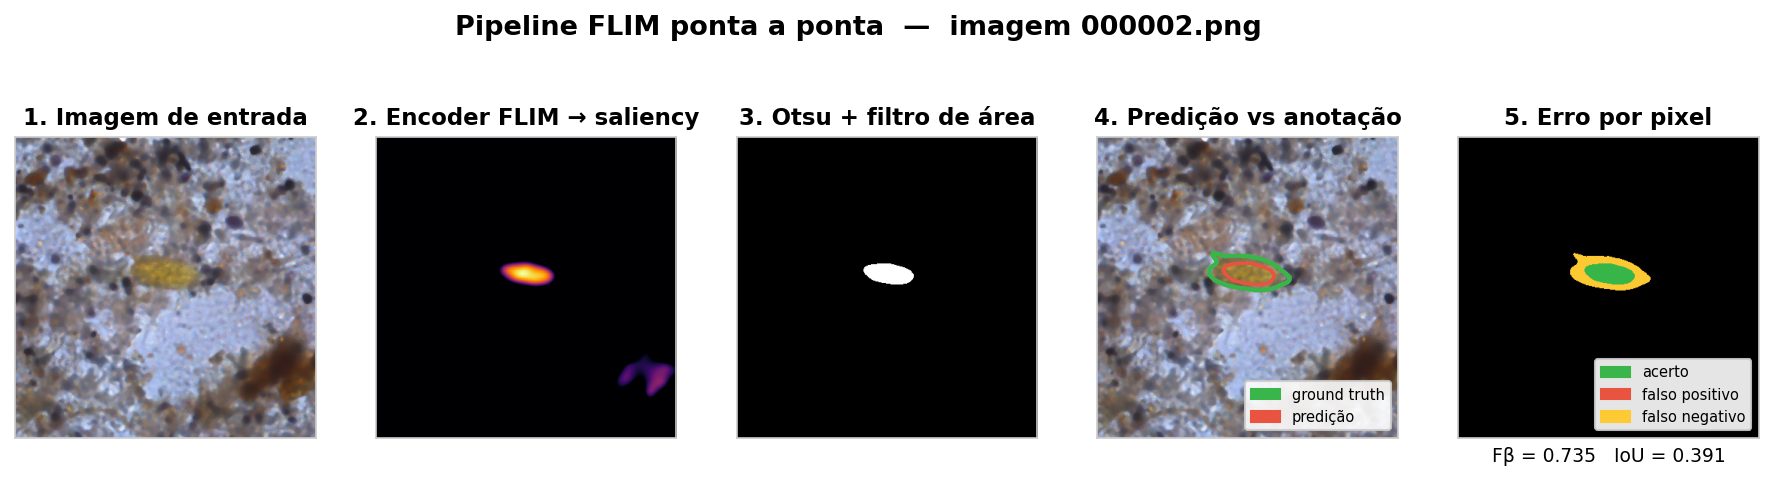
\includegraphics[width=\linewidth]{flim_pipeline.png}
\caption[O \acs{FLIM} de ponta a ponta numa imagem]{O método de ponta a ponta. A imagem de entrada passa pelo codificador, que produz o mapa de saliência; a limiarização de Otsu com filtro de área produz a máscara binária; a comparação com a anotação de referência dá o $F_\beta$ e o \ac{IoU}. O último painel decompõe o erro em falso positivo e falso negativo.}
\label{fig_pipeline}
\end{figure}

Vale também fixar o que é um marcador, já que ele é a única entrada de supervisão do método. A Figura~\ref{fig_markers} contrasta o traço desenhado por um especialista com o traço sintético usado nas campanhas que precisam de mais imagens anotadas do que as 31 para as quais existe marcação real.

\begin{figure}[htb]
\centering
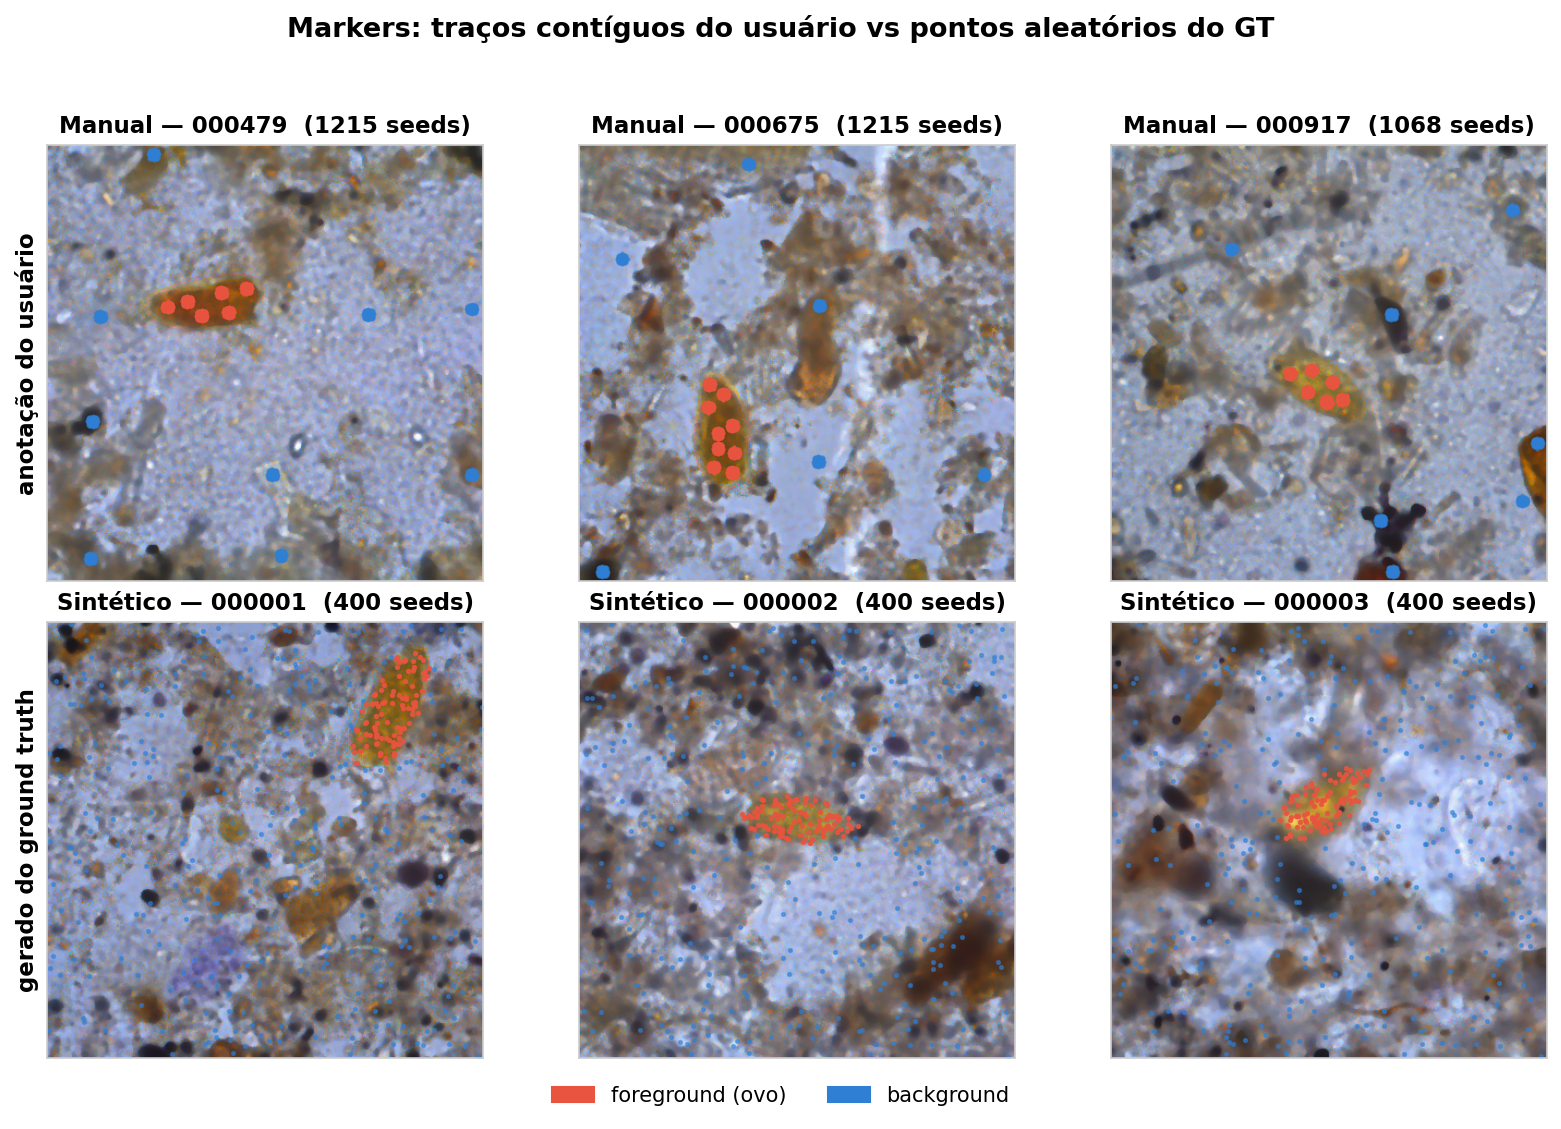
\includegraphics[width=\linewidth]{flim_markers.png}
\caption[Marcador real e marcador sintético]{O que o método recebe como supervisão. À esquerda o traço real de um especialista; à direita o traço sintético gerado a partir da anotação de referência. A distinção importa porque marcador real existe apenas para 31 imagens do conjunto de parasitas, e comparações entre braços de origens diferentes mediriam quem desenhou o traço em vez do efeito em estudo.}
\label{fig_markers}
\end{figure}

\section{Métricas}

\subsection{Qualidade da segmentação}

A métrica principal é o $F_\beta$, que combina precisão e revocação com peso maior para a precisão, seguindo o trabalho de referência:

\begin{equation}
F_\beta = \frac{(1 + \beta^2) \cdot P \cdot R}{\beta^2 \cdot P + R}, \qquad \beta^2 = 0{,}3
\label{eq_fbeta}
\end{equation}

onde $P$ é a precisão e $R$ a revocação, calculadas pixel a pixel sobre a máscara binarizada.

Reporta-se também a \ac{IoU}, razão entre a interseção e a união das máscaras predita e verdadeira:

\begin{equation}
\text{IoU} = \frac{|\hat{Y} \cap Y|}{|\hat{Y} \cup Y|}
\label{eq_iou}
\end{equation}

A acurácia pixel a pixel é reportada por completude, mas não discrimina neste domínio: como os objetos ocupam pequena fração da imagem, predizer tudo como fundo já produz acurácia superior a $0{,}97$.

\subsection{Esforço de interação}

Para a avaliação interativa usa-se o \ac{NoC}, número de cliques necessários para que a \ac{IoU} ultrapasse um alvo $\tau$, com um teto $N_{\max}$ de interações:

\begin{equation}
\text{NoC@}\tau = \min\{\,n \leq N_{\max} : \text{IoU}_n \geq \tau\,\},
\quad \text{ou } N_{\max} \text{ se nenhum } n \text{ satisfaz}
\label{eq_noc}
\end{equation}

Imagens que não atingem o alvo entram na média com o valor do teto. Por isso a taxa de sucesso é reportada ao lado do \ac{NoC} em todas as tabelas: um método poderia exibir contagem baixa simplesmente por desistir antes, e a contagem isolada premiaria esse comportamento.

\section{Aprendizado ativo}
\label{sec_al_metodo}

\subsection{O problema que o aprendizado ativo resolve}

Anotar uma imagem para segmentação custa caro. Quem anota precisa ser um especialista, o traço precisa acompanhar a fronteira do objeto, e o tempo gasto cresce com a quantidade de imagens. O conjunto de parasitas usado aqui tem 1220 lâminas; anotar todas é inviável na prática e desnecessário em princípio, porque muitas são parecidas entre si e o modelo não aprende nada de novo com a segunda cópia de algo que já viu.

O \ac{AL} parte dessa observação. Em vez de anotar tudo ou sortear ao acaso, ele usa o modelo já treinado para decidir o que vale a pena anotar em seguida. O procedimento é um laço:

\begin{enumerate}
    \item treina-se um modelo com o pouco que já está anotado, o conjunto $A$;
    \item aplica-se esse modelo ao que ainda não foi anotado, o conjunto $U$, chamado \emph{pool};
    \item uma função de aquisição $s(\cdot)$ atribui uma pontuação a cada candidato de $U$;
    \item o candidato de maior pontuação vai para o especialista, que o anota;
    \item ele passa de $U$ para $A$, e o laço recomeça.
\end{enumerate}

A função de aquisição é o que distingue um método de \ac{AL} de outro. Todo o resto do laço é igual.

\subsection{O custo de pontuar o pool, e por que ele importa aqui}
\label{sec_custo_pool}

Há um detalhe que a literatura de \ac{AL} costuma tratar como secundário e que, no caso do \ac{FLIM}, é central: \textbf{pontuar o pool também custa}. A pergunta não é só quantas imagens o especialista anota, é também o que a máquina precisa fazer, e precisa saber, para decidir quais são.

Os critérios avaliados nesta dissertação se separam em três faixas de custo, e a distinção importa porque o \ac{FLIM} existe justamente para funcionar quando não se tem anotação em massa:

\begin{description}
    \item[Uma passagem pelo pool, sem anotação.] Entropia, \ac{LC} e margem precisam apenas da predição do modelo atual sobre cada imagem de $U$. O custo é uma inferência por imagem, e nenhuma anotação é consultada. É a faixa mais barata.

    \item[Várias passagens, ou atributos de todo o pool, sem anotação.] O \ac{BALD} exige um comitê, logo $N$ inferências por imagem. O CoreSet e o \ac{BADGE} exigem extrair o vetor de atributos de \emph{cada} imagem do pool e depois resolver um problema de cobertura sobre todos eles. Continuam sem consultar anotação, mas o custo cresce com o tamanho do pool, e não apenas com o orçamento.

    \item[Anotação de todo o pool.] É o caso do passo 7 do Algoritmo 1 do trabalho de referência, que escolhe a próxima imagem entre as de pior $F_\beta$. Para saber o $F_\beta$ de uma imagem é preciso ter o gabarito dela. Escolher 3 imagens entre 848 exige, portanto, as 848 anotadas.
\end{description}

Esta última linha é a razão de ser desta dissertação. O próprio artigo declara que a abordagem de seleção é supervisionada, e um procedimento que precisa do gabarito de todo o pool para escolher o que anotar derrota o propósito de um método criado para operar com três a cinco imagens anotadas. A pergunta que organiza o trabalho é, então, quanto do benefício daquele procedimento se recupera com critérios da primeira e da segunda faixa, que não consultam anotação nenhuma.

Por isso o Algoritmo 1 aparece aqui sob o nome de \textbf{baseline supervisionado com informação privilegiada}, e não como método concorrente: ele tem acesso a uma informação que os demais não têm.

Convém ser explícito quanto ao que esse braço \emph{não} é. Consultar a anotação de referência não transforma automaticamente uma heurística em limite superior de desempenho. Um limite superior exigiria que o procedimento maximizasse o desfecho avaliado, e o Algoritmo 1 maximiza outra coisa: ele escolhe a imagem de \emph{pior} $F_\beta$, que não é necessariamente a mais informativa. A medição relatada no Capítulo~\ref{cap_4} mostra que ele pode, inclusive, perder para o sorteio aleatório. Os termos \emph{teto} e \emph{limite superior} são, portanto, evitados para esse braço ao longo de todo o trabalho.

\subsection{Critérios de incerteza}
\label{sec_crit_incerteza}

A família de incerteza parte da ideia de que o modelo aprende mais com aquilo sobre o que está em dúvida. Se a predição já é confiante, anotar aquela imagem apenas confirma o que o modelo já sabe.

\paragraph{Uma ressalva de nomenclatura, antes das fórmulas.} Seja $S(x,y) \in [0,1]$ o valor que o decodificador atribui ao pixel $(x,y)$. Esse valor é o \textbf{escore de saliência normalizado}: ele resulta da normalização linear do mapa de ativação da Equação~\ref{eq_decoder} para o intervalo unitário, e é armazenado quantizado em oito bits. Ele \textbf{não é uma probabilidade calibrada}. Não provém de uma função logística ajustada, não passou por calibração, e nada garante que o valor $0{,}6$ corresponda a 60\% de chance de o pixel ser objeto.

As funções de aquisição abaixo são, portanto, aplicadas a $S$ \emph{por analogia} com a formulação probabilística, e o termo \emph{pseudo-probabilidade} é usado ao longo do texto para marcar essa distinção. Duas consequências decorrem disso e valem ser enunciadas. A primeira é que a entropia calculada sobre $S$ não deve ser lida como incerteza epistêmica calibrada: o máximo em $S = 0{,}5$ é uma propriedade de onde a normalização situa o ponto médio, e não de uma dúvida probabilística do modelo. A segunda é que as comparações entre braços permanecem válidas, porque todos os braços recebem exatamente a mesma representação, e a diferença entre eles isola o critério e não a escala.

A \textbf{entropia} mede a indecisão ponto a ponto, atingindo o máximo quando o escore é exatamente $0{,}5$:

\begin{equation}
H(x,y) = -\big[S \log S + (1-S)\log(1-S)\big]
\label{eq_entropia}
\end{equation}

O \textbf{least confidence} mede a distância à fronteira de decisão. A intuição é a mesma da entropia, com escala diferente:

\begin{equation}
\text{LC}(x,y) = 1 - |2S - 1|
\label{eq_lc}
\end{equation}

A \textbf{margem}, em classificação multiclasse, é a diferença entre as duas classes mais prováveis. No caso binário só existem duas classes, e a definição colapsa exatamente na de \emph{least confidence}. Os dois critérios foram mantidos separados nos experimentos porque a literatura os trata como distintos, mas a equivalência algébrica no caso binário precisa ser dita: \textbf{qualquer diferença observada entre eles nos resultados é ruído de execução, não efeito de critério}.

Os três critérios acima medem a incerteza de \emph{um} modelo, e essa incerteza mistura duas coisas diferentes. Um pixel pode ser ambíguo porque a imagem é genuinamente ambígua naquele ponto, ou porque o modelo está mal treinado. Anotar o segundo caso ajuda; anotar o primeiro não resolve, porque nenhuma quantidade de dados elimina ambiguidade intrínseca.

O quarto critério desta família, aqui denominado \textbf{critério inspirado em \ac{BALD} por discordância de comitê}, separa as duas usando o desacordo entre modelos. Dado um comitê de $N$ modelos com predições $p_1, \dots, p_N$:

\begin{equation}
\text{BALD} = H\!\left(\frac{1}{N}\sum_i p_i\right) - \frac{1}{N}\sum_i H(p_i)
\label{eq_bald}
\end{equation}

O primeiro termo é a incerteza total e o segundo é a parcela que todos os modelos compartilham. A diferença isola o desacordo: um ponto em que todos os modelos estão inseguros da mesma forma recebe pontuação baixa, e um ponto em que eles discordam entre si recebe pontuação alta.

A formulação original do \ac{BALD} é bayesiana: o comitê aproxima a posterior sobre os parâmetros, obtida por \emph{dropout} de Monte Carlo com várias passagens estocásticas pelo mesmo modelo, e a quantidade medida é o ganho de informação esperado sobre essa posterior. \textbf{O \ac{FLIM} não tem \emph{dropout} e sua inferência é determinística}, de modo que essa via não existe aqui, e não há posterior a aproximar.

O que este trabalho mede é, portanto, \emph{discordância entre codificadores distintos}, usando como comitê os mapas de saliência de cada um. A quantidade da Equação~\ref{eq_bald} continua bem definida e continua separando desacordo de incerteza compartilhada, mas ela \textbf{não é uma aproximação bayesiana}, e o texto evita chamá-la de \ac{BALD} sem qualificação. A leitura dos resultados correspondentes deve ser feita nesses termos.

\subsection{Critérios de diversidade}
\label{sec_crit_diversidade}

A família de diversidade parte de uma objeção à anterior. Escolher sempre o mais incerto tende a escolher repetidamente o mesmo tipo de caso difícil, e um lote de imagens parecidas entre si ensina pouco mais do que uma delas. Os critérios de diversidade ignoram a incerteza e olham a \emph{cobertura}: o objetivo é que o conjunto anotado represente bem o conjunto todo.

Cada candidato é descrito por um vetor $f(\cdot)$ obtido pela média das ativações do codificador dentro da sua máscara.

O \textbf{CoreSet} formula a seleção como cobertura geométrica, escolhendo o candidato mais distante de tudo o que já foi anotado, que é o passo guloso do $k$-center:

\begin{equation}
r^{\ast} = \arg\max_{r \notin A} \; \min_{a \in A} \; \lVert f(r) - f(a) \rVert_2
\label{eq_coreset}
\end{equation}

onde $A$ é o conjunto já anotado e $f(\cdot)$ o vetor de atributos. Lê-se de dentro para fora: para cada candidato, encontre o item já anotado mais próximo dele; depois escolha o candidato cuja menor distância é a maior de todas. Em palavras, o candidato que está na região mais desassistida do espaço de atributos.

O \textbf{medoide} faz o oposto, escolhendo o candidato mais típico, o de menor distância média a todos os demais:

\begin{equation}
r^{\ast} = \arg\min_{r} \; \frac{1}{|R|}\sum_{q \in R} \lVert f(r) - f(q) \rVert_2
\label{eq_medoide}
\end{equation}

Ele entrou nos experimentos como contraste deliberado ao CoreSet. Se a cobertura de regiões extremas fosse o que importa, o medoide deveria ir pior que o CoreSet; se o que importasse fosse representatividade, o contrário. Ter os dois permite distinguir as hipóteses, em vez de apenas constatar que um critério não funcionou.

O terceiro critério de diversidade avaliado é um \textbf{híbrido inspirado no \ac{BADGE}}, e a qualificação não é cosmética: a implementação usada aqui diverge da formulação original de uma forma que precisa ser declarada.

A ideia do \ac{BADGE} é construir um vetor que carregue incerteza e diversidade ao mesmo tempo, aplicando o $k$-means++ sobre \emph{embeddings de gradiente}. No método original, o embedding é o gradiente da perda em relação à última camada, avaliado no pseudo-rótulo $\hat{y} = \arg\max_k P_k$:

\begin{equation}
g_i^{\text{original}} = \big(P_i - e_{\hat{y}}\big) \otimes f(r_i)
\label{eq_badge_original}
\end{equation}

cuja magnitude, no caso binário, é proporcional a $|P_i - \operatorname{round}(P_i)|$, isto é, \emph{máxima} quando $P_i$ se aproxima de $0{,}5$ e próxima de zero quando o modelo está confiante. A implementação avaliada neste trabalho usa, em seu lugar:

\begin{equation}
g_i = \big(S_i - \tfrac{1}{2}\big)\, f(r_i)
\label{eq_badge}
\end{equation}

cuja magnitude é $|S_i - 0{,}5|$, ou seja, \textbf{nula} na incerteza máxima e \emph{máxima} na confiança máxima. Como o $k$-means++ sorteia pontos com probabilidade proporcional ao quadrado da distância, o efeito é favorecer os candidatos mais \emph{confiantes}, invertendo a intenção do método original.

A divergência foi identificada na auditoria do código e está registrada aqui em vez de corrigida porque este critério \textbf{não participa de nenhum resultado central} desta dissertação: ele aparece somente na tabela que reúne todas as técnicas avaliadas, e não nas campanhas de ganho marginal, de custo do aprendizado ativo ou de troca do gerador. A leitura correta da linha correspondente é, portanto, que \emph{um híbrido de diversidade ponderado por confiança} não superou o sorteio, e não que o \ac{BADGE} tenha sido avaliado. Reimplementar a Equação~\ref{eq_badge_original} e reexecutar essa comparação consta entre os trabalhos futuros do Capítulo~\ref{cap_5}.

\subsection{Por que estes critérios, e não outros}

A escolha não foi por conveniência de implementação. O conjunto avaliado cobre as posições que a literatura ocupa, com um representante de cada e com os controles que permitem distingui-las:

\begin{itemize}
    \item \textbf{incerteza pura}: entropia, \ac{LC} e margem;
    \item \textbf{incerteza corrigida por desacordo}: \ac{BALD};
    \item \textbf{diversidade pura}: CoreSet e medoide, em direções opostas;
    \item \textbf{híbrido}: \ac{BADGE};
    \item \textbf{baseline privilegiado}: o procedimento do trabalho de referência, que lê o gabarito e reproduz o passo 7 do Algoritmo 1;
    \item \textbf{piso}: sorteio aleatório, sem critério nenhum.
\end{itemize}

O piso e o baseline privilegiado são o que torna o conjunto interpretável. Sem o sorteio não se sabe se um critério ajudou ou se qualquer escolha teria ajudado. Sem o baseline privilegiado não se sabe se a dificuldade está em o critério ser imperfeito ou em a seleção de imagem não ser a alavanca certa, e é essa distinção que os resultados do Capítulo~\ref{cap_4} acabam decidindo.

Ficaram de fora os métodos que exigem retropropagação para funcionar, como os baseados em gradiente da perda ou em redes adversárias de seleção. Não é omissão: o \ac{FLIM} não tem perda nem otimizador, e esses métodos não são aplicáveis sem descaracterizar o modelo que está sendo estudado.

\subsection{Seleção de imagem e seleção de região}
\label{sec_imagem_vs_regiao}

Os critérios acima foram aplicados em dois níveis, e os dois níveis respondem a perguntas diferentes. Confundi-los é o erro mais fácil de cometer ao ler os resultados.

Na \textbf{seleção de imagem}, o candidato é a imagem inteira e a pontuação é a média do critério sobre todos os seus pixels. O que se decide é \emph{quais imagens} o especialista vai anotar. É a forma usual na literatura e é a que o Algoritmo 1 do trabalho de referência usa. A Figura~\ref{fig_al_imagem} mostra o que o critério enxerga nesse nível.

\begin{figure}[htb]
\centering
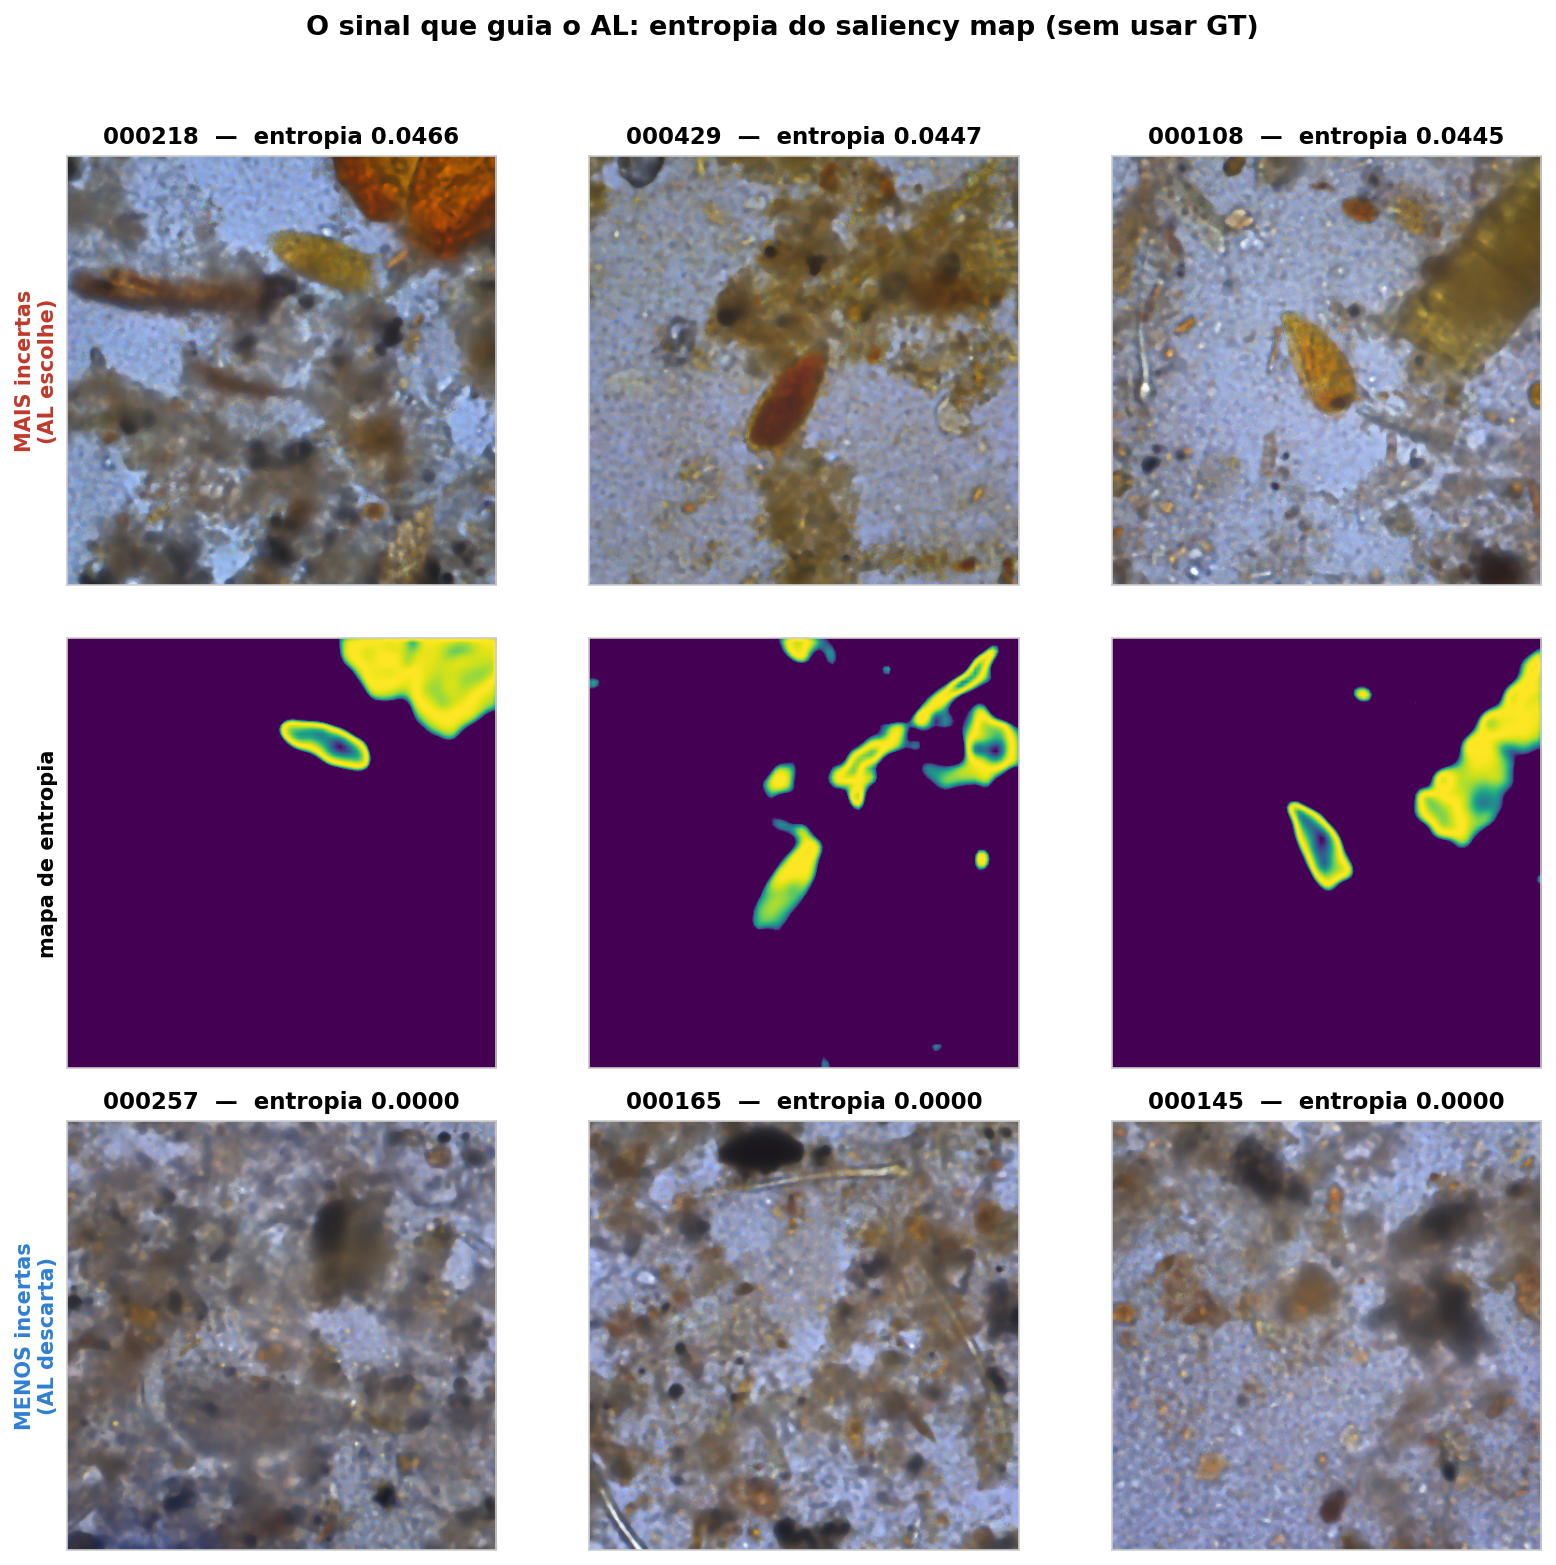
\includegraphics[width=\linewidth]{al_selecao_imagem.png}
\caption[O que o critério de incerteza enxerga no nível de imagem]{Seleção no nível de imagem. À esquerda, o mapa de entropia produzido pelo codificador; à direita, as imagens do pool com maior e menor pontuação. A pontuação de uma imagem é a média do critério sobre todos os seus pixels, de modo que o fundo, que ocupa a maior parte da área, domina o valor.}
\label{fig_al_imagem}
\end{figure}

Na \textbf{seleção de região}, a imagem é particionada em regiões e o candidato é uma região. A pontuação é a média do critério dentro dela:

\begin{equation}
s(r) = \frac{1}{|r|} \sum_{(x,y) \in r} H(x,y)
\label{eq_score_regiao}
\end{equation}

O que se decide aqui é \emph{onde}, dentro de imagens já escolhidas, o traço vai cair. O braço de região usa exatamente as mesmas imagens que o sorteio usaria e gasta exatamente a mesma quantidade de pixels marcados. A única variável é a posição. A Figura~\ref{fig_al_regiao} mostra o procedimento completo.

\begin{figure}[htb]
\centering
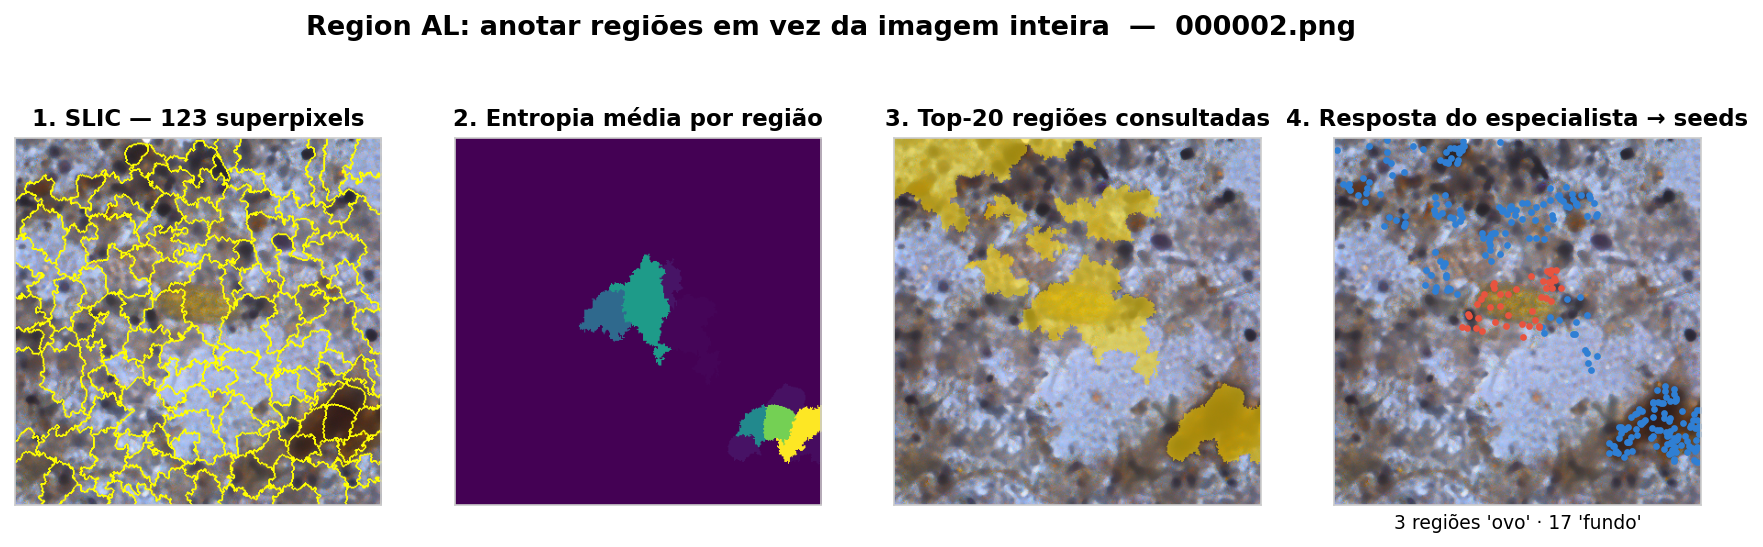
\includegraphics[width=\linewidth]{al_regiao_slic.png}
\caption[Aprendizado ativo no nível de região]{Seleção no nível de região, passo a passo: a imagem é particionada pelo \ac{SLIC}, cada superpixel recebe a média do critério dentro dele, as regiões mais bem pontuadas são apresentadas ao especialista, e a resposta dele vira marcadores de objeto e de fundo. As mesmas imagens e o mesmo orçamento de pixels do braço de sorteio; o que muda é a posição.}
\label{fig_al_regiao}
\end{figure}

A consequência prática é que \textbf{as duas diferenças não são comparáveis entre si}. O $\Delta$ da seleção de imagem mede escolha de imagem; o $\Delta$ da seleção de região mede posição de anotação. Somá-los ou apresentá-los na mesma coluna mediria duas coisas ao mesmo tempo.

A extensão do CoreSet e do medoide ao nível de região é contribuição deste trabalho. Na literatura esses dois critérios são de imagem por construção, pois comparam imagens inteiras. A adaptação substitui a média global das ativações pela média dentro da máscara de cada região, mantendo o mesmo espaço de atributos e o mesmo passo guloso.

\subsection{Geração dos candidatos}
\label{sec_gerador}

A pontuação só ordena a lista de candidatos que recebe, de modo que o procedimento que gera essa lista é parte do método, e não detalhe de implementação. Dois geradores são comparados nesta dissertação.

O primeiro, usual na literatura, particiona a imagem em superpixels pelo algoritmo \ac{SLIC}, e cada superpixel é um candidato. O segundo, proposto aqui, define cada candidato como um disco de raio $\rho$ centrado em um ponto do contorno predito:

\begin{equation}
\partial \hat{Y} = \hat{Y} \setminus \operatorname{erosão}(\hat{Y}), \qquad
r_i = \{(x,y) : \lVert (x,y) - c_i \rVert_2 \leq \rho,\; c_i \in \partial \hat{Y}\}
\label{eq_contorno}
\end{equation}

onde $\hat{Y}$ é a máscara predita. Os centros $c_i$ são amostrados sobre o contorno com espaçamento mínimo de $2\rho$, para que os discos se toquem sem se sobrepor. O contorno usado é o \emph{predito}, e não o verdadeiro, de modo que o procedimento não depende de anotação prévia.

A Figura~\ref{fig_gerador} mostra o contraste entre os dois geradores na mesma imagem. A diferença não é de escore: é de qual lista o escore recebe.

\begin{figure}[htb]
\centering
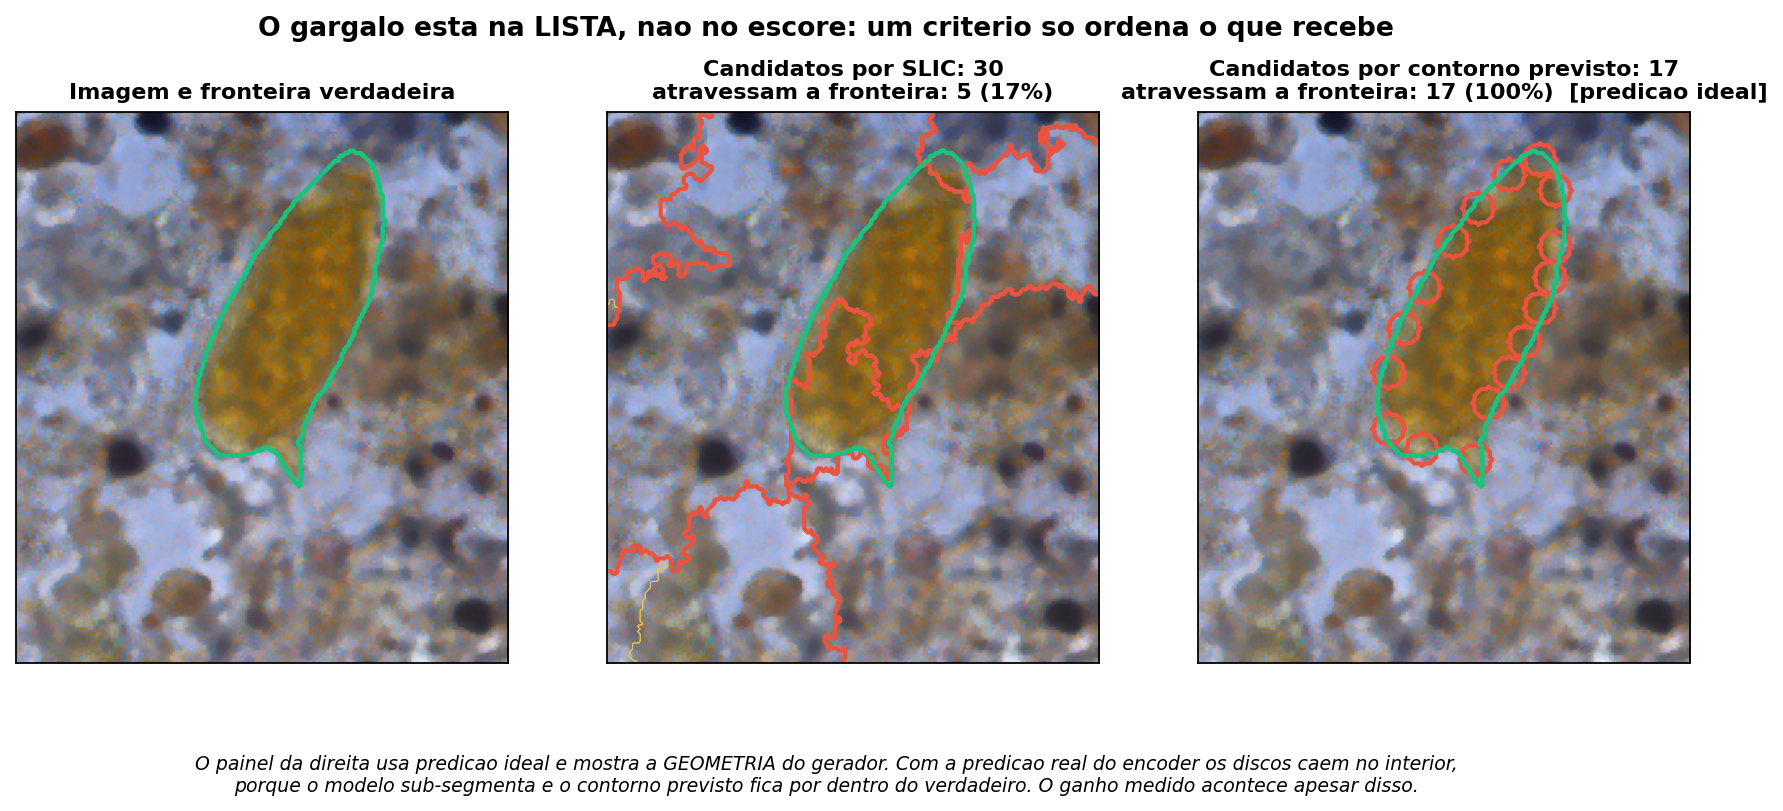
\includegraphics[width=\linewidth]{gerador_candidatos.png}
\caption[Superpixels e discos de contorno como geradores de candidatos]{Os dois geradores de candidatos na mesma imagem. As arestas do \ac{SLIC} seguem as bordas presentes na imagem por construção, de modo que seus pedaços tendem a ficar de um lado só da fronteira do objeto; os discos centrados no contorno cobrem os dois lados por construção. O painel da direita usa predição ideal e ilustra a geometria do gerador: com a predição real do codificador os discos caem no interior, porque o modelo sub-segmenta e o contorno predito fica por dentro do verdadeiro, e o ganho medido no Capítulo~\ref{cap_4} acontece apesar disso.}
\label{fig_gerador}
\end{figure}

Uma limitação do gerador proposto precisa ser registrada junto com ele, porque é consequência direta do seu desenho. Ele depende de haver um contorno predito: com máscara predita vazia ou cheia, o conjunto de candidatos sai vazio, enquanto o \ac{SLIC} funciona sempre. E a dependência não aparece apenas no caso extremo. Quando o contorno predito é curto, o espaçamento mínimo de $2\rho$ limita quantos centros cabem, e o gerador entrega \emph{menos} candidatos do que os pedidos. Isso foi observado em três sementes das campanhas e tem consequência estatística, tratada no Capítulo~\ref{cap_4}.

\section{Aprendizado contínuo}

\subsection{O esquecimento no FLIM}\label{sec_cl_flim}

Os métodos consolidados de \ac{CL} supõem um modelo treinado por gradiente, e atuam sobre o deslocamento dos pesos durante o ajuste. Como o \ac{FLIM} não possui otimizador, nenhum deles se aplica diretamente.

O fenômeno análogo, contudo, está na Equação \ref{eq_nivel2}. Sejam $C_t$ o conjunto de candidatos na rodada $t$ e $K_t$ o banco de filtros resultante. Acrescentar marcadores produz $C_{t+1} \supset C_t$, e como o agrupamento é refeito sobre o conjunto ampliado, não há garantia de que $K_{t+1}$ preserve qualquer elemento de $K_t$. Além disso, $K_t$ é compartilhado por todas as imagens, inclusive as não anotadas, de modo que a perturbação é global.

\subsection{O mecanismo de retenção}

A intervenção proposta interpola o banco em vez de substituí-lo. Para cada centróide novo $k \in K_{t+1}$, localiza-se o centróide anterior mais próximo e produz-se uma combinação convexa:

\begin{equation}
\tilde{k} = (1 - \alpha)\,\operatorname{anc}(k) + \alpha\,k,
\qquad
\operatorname{anc}(k) = \arg\min_{k' \in K_t} \lVert k - k' \rVert_2
\label{eq_retencao}
\end{equation}

O parâmetro $\alpha \in [0,1]$ é a taxa de plasticidade. Com $\alpha = 1$ o procedimento reproduz o \ac{FLIM} original. Com $\alpha = 0$ o banco passa a conter apenas direções já presentes em $K_t$, e nenhuma informação nova entra. Valores intermediários deslocam o banco parcialmente na direção da nova estimativa.

A âncora é tomada por centróide \emph{novo}, e não por centróide anterior. A direção importa: ancorar no sentido oposto obrigaria a saída a ter o tamanho do banco anterior, o que conflita com o ajuste automático do número de canais descrito na Equação \ref{eq_regimes} e invalida as estatísticas de normalização recalculadas a cada rodada.

\section{Aprendizado interativo}

\subsection{O usuário simulado}

Avaliar refinamento interativo exige um procedimento reprodutível que decida onde o especialista clicaria. Adota-se o protocolo consolidado por \cite{xu2016deep_arxiv}, no qual o clique vai ao centro do maior erro.

O erro é separado em dois tipos. O falso negativo, $\text{FN} = Y \setminus \hat{Y}$, indica região de objeto que o modelo não detectou e gera clique de objeto. O falso positivo, $\text{FP} = \hat{Y} \setminus Y$, indica região de fundo marcada como objeto e gera clique de fundo. Entre as componentes conexas desses dois conjuntos, escolhe-se a de maior área.

Dentro da componente escolhida, o clique \textbf{não} vai ao centróide. Vai ao ponto de máxima transformada de distância:

\begin{equation}
c^{\ast} = \arg\max_{(x,y) \in E} \; D_E(x,y)
\label{eq_clique}
\end{equation}

onde $E$ é a componente de erro e $D_E(x,y)$ é a distância euclidiana de $(x,y)$ à borda de $E$. Essa escolha não é arbitrária. O centróide de uma região côncava pode cair fora dela, o que produziria um clique com rótulo errado; e mesmo em região convexa o centróide não é necessariamente o ponto mais afastado da borda. O ponto de máxima distância está, por construção, no interior e o mais longe possível da franja, onde a atribuição de rótulo seria ambígua.

O clique é materializado como um disco de raio 5 pixels, valor medido nos 31 conjuntos de marcadores reais disponíveis, recortado de modo a não ultrapassar a fronteira do objeto. Não há sorteio em nenhuma etapa do laço, de forma que o \ac{NoC} é determinístico dado o codificador inicial.

A Figura~\ref{fig_clique} percorre esse procedimento numa imagem real e mostra por que a distinção entre centróide e máxima distância não é preciosismo. No exemplo, a região de erro tem forma de anel, e o centróide cai no vazio central, isto é, \emph{fora} da região que deveria rotular.

\begin{figure}[htb]
\centering
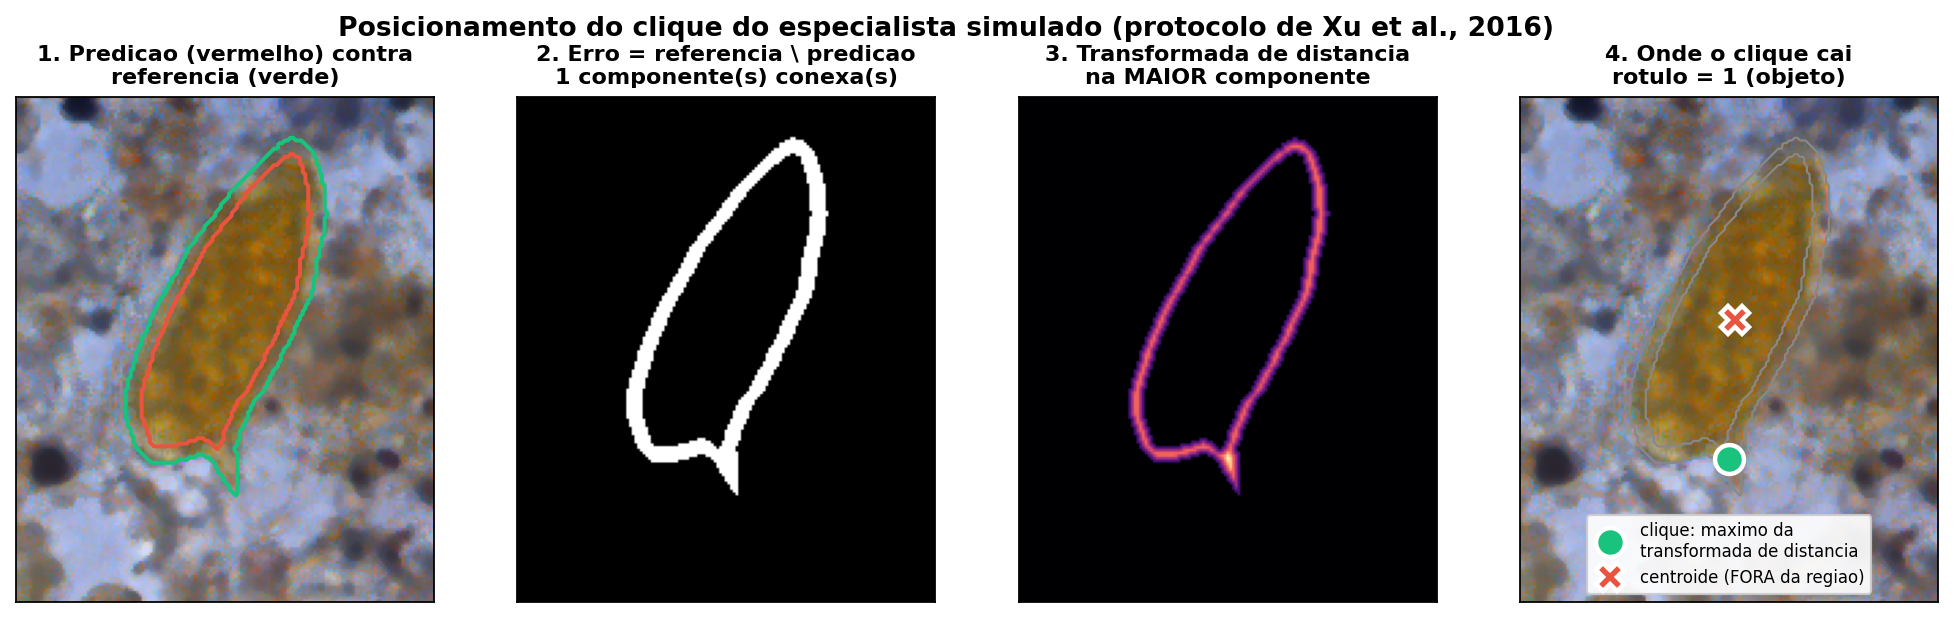
\includegraphics[width=\linewidth]{il_clique.png}
\caption[Posicionamento do clique do usuário simulado]{Como o clique é posicionado. A diferença entre a predição e a anotação de referência define a região de erro; dentro da maior componente conexa dela, o clique vai ao máximo da transformada de distância. Neste exemplo a região de erro é um anel e o centróide cai fora dela, que é exatamente o caso que a Equação~\ref{eq_clique} evita.}
\label{fig_clique}
\end{figure}

\subsection{O laço}

A cada iteração, o modelo prediz, o usuário simulado escolhe o clique, o marcador é acrescentado, o codificador é reestimado com a plasticidade configurada, e a \ac{IoU} é medida novamente. O laço termina quando a \ac{IoU} ultrapassa o alvo ou quando o teto de cliques é atingido.

O laço possui dois pontos em que os componentes se encaixam. O \ac{AL} pode reordenar os candidatos a clique, em lugar de sempre tomar o maior erro, e o \ac{CL} controla como o clique é incorporado, pelo parâmetro $\alpha$ da Equação \ref{eq_retencao}.

\section{A plataforma interativa}

Os experimentos descritos neste capítulo são executados em lote, com usuário simulado. Para observar o comportamento do sistema com uma pessoa real no laço, foi desenvolvida uma aplicação que roda localmente e integra os três componentes em um fluxo único.

A aplicação é um servidor em Python servindo uma página única, sem dependência de serviço externo. Ela é iniciada em linha de comando e atendida em \texttt{localhost}, de modo que as imagens, que são dados de pacientes em dois dos três conjuntos, não saem da máquina. A interface se organiza em cinco abas, descritas a seguir.

\subsection{Os conjuntos disponíveis e o envio de novos}

A aba de conjuntos lista o que está disponível e permite enviar um conjunto novo, conforme a Figura~\ref{fig_plat_datasets}. O padrão adotado é um diretório com \texttt{orig/} e, opcionalmente, \texttt{label/}. A anotação de referência é opcional de propósito: um conjunto trazido por um especialista normalmente não tem anotação nenhuma, que é precisamente a situação que o método endereça. Sem \texttt{label/} a aplicação continua treinando e prevendo, e o que deixa de existir é o cálculo automático do $F_\beta$, passando a avaliação a ser o julgamento visual de quem usa.

\begin{figure}[htb]
\centering
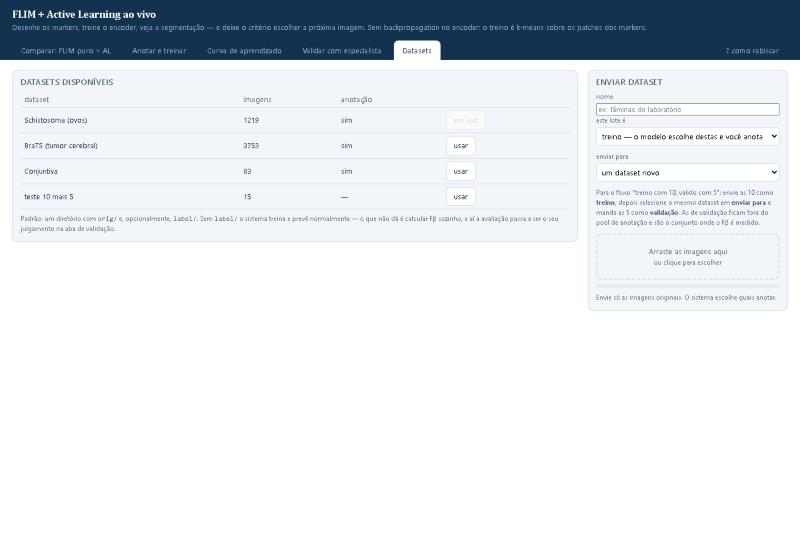
\includegraphics[width=\linewidth]{plataforma_datasets.jpg}
\caption[Aba de conjuntos de dados da plataforma]{A aba de conjuntos. Além dos três conjuntos usados nos experimentos, a aplicação aceita o envio de um conjunto novo, com ou sem anotação de referência, e permite separar o lote entre treino e validação no momento do envio.}
\label{fig_plat_datasets}
\end{figure}

\subsection{O ciclo}

A aplicação opera em rodadas. A cada rodada, o estado consiste no conjunto de marcadores acumulados, no codificador estimado a partir deles, e na curva de qualidade registrada até ali.

O \ac{AL} atua na etapa de sugestão: a aplicação calcula o mapa de probabilidade, pontua as regiões candidatas, e apresenta ao especialista a de maior incerteza. O especialista decide se aceita a sugestão ou se marca outro ponto, e informa se a região é objeto ou fundo. O \ac{IL} atua na incorporação: o toque é materializado como disco de raio 5, acrescentado ao conjunto de marcadores, e o codificador é reestimado. O \ac{CL} atua no controle da reestimação, pelo parâmetro de plasticidade da Equação \ref{eq_retencao}, que pode ser alterado \emph{entre} rodadas.

Essa última possibilidade é deliberada. Alterar a plasticidade no meio de uma sessão permite comparar os dois comportamentos sobre a mesma imagem e o mesmo histórico de cliques, o que torna a diferença visível sem exigir duas sessões separadas.

A Figura~\ref{fig_plat_anotar} mostra a tela desse ciclo. À esquerda ficam o pincel de objeto, o pincel de fundo e a imagem que o critério escolheu; à direita, o estado da rodada, o orçamento configurado, o decodificador e o critério em uso, e um registro textual que explica, a cada passo, \emph{por que} aquela imagem foi escolhida. Esse registro é deliberado: sem ele a escolha do sistema é uma caixa preta para quem anota, e a aplicação existe para tornar o mecanismo observável.

\begin{figure}[htb]
\centering
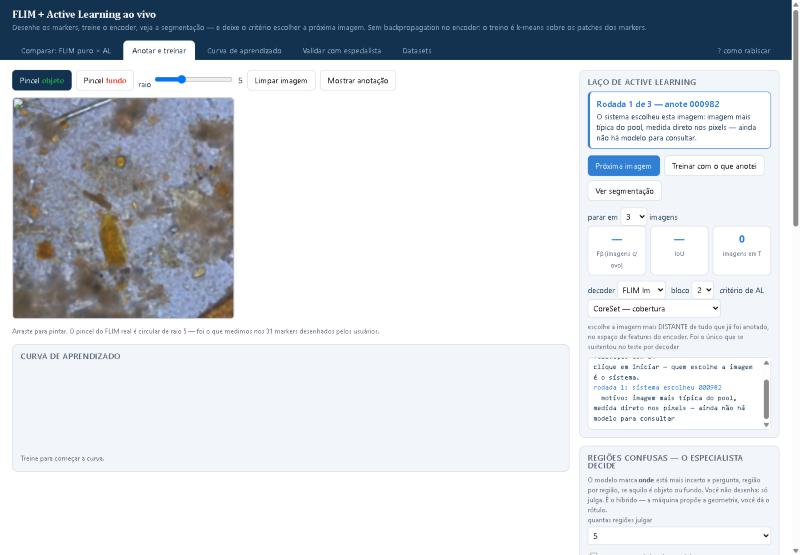
\includegraphics[width=\linewidth]{plataforma_anotar.jpg}
\caption[Tela de anotação e treino da plataforma]{A tela de anotação. O painel da direita mostra a rodada corrente, o motivo da escolha da imagem, o orçamento, o decodificador e o critério de \ac{AL}. Abaixo dele fica o painel de regiões confusas, pelo qual o modelo pergunta e o especialista decide.}
\label{fig_plat_anotar}
\end{figure}

\subsection{A comparação entre braços na própria tela}

Duas comparações do Capítulo~\ref{cap_4} estão implementadas na aplicação, e é por elas que ela deixa de ser apenas uma demonstração de interface.

A primeira, na Figura~\ref{fig_plat_comparar}, põe o \ac{FLIM} com sorteio de imagens contra um ou mais critérios de \ac{AL}, com o mesmo orçamento e o mesmo conjunto de validação. Um detalhe do desenho merece nota: a imagem da primeira rodada é comum a todos os braços, e o traço feito nela vale para todos. Sem isso, a diferença observada no fim incluiria qual imagem calhou de sair primeiro para cada braço, que é a maior fonte de variância do método.

\begin{figure}[htb]
\centering
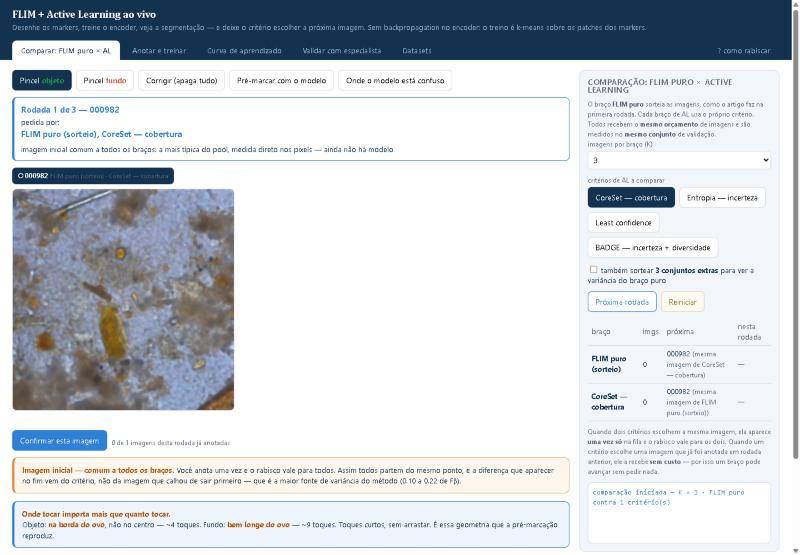
\includegraphics[width=\linewidth]{plataforma_comparar.jpg}
\caption[Comparação entre \acs{FLIM} puro e Active Learning na plataforma]{A comparação entre braços. Todos recebem o mesmo orçamento de imagens e são medidos no mesmo conjunto de validação. Quando dois critérios escolhem a mesma imagem, ela aparece uma vez só na fila e a anotação vale para ambos.}
\label{fig_plat_comparar}
\end{figure}

A segunda, na Figura~\ref{fig_plat_onde}, é a que corresponde à contribuição central desta dissertação. Ela mantém as mesmas imagens em todos os braços e o mesmo número de pixels marcados, e varia apenas \emph{quem escolhe o lugar}: o especialista, o modelo por pré-marcação, o critério de \ac{AL} por região, ou o sorteio. É o braço de sorteio que torna os outros interpretáveis, porque sem ele não há como separar o ganho de escolher bem a região do ganho de simplesmente anotar em blocos.

\begin{figure}[htb]
\centering
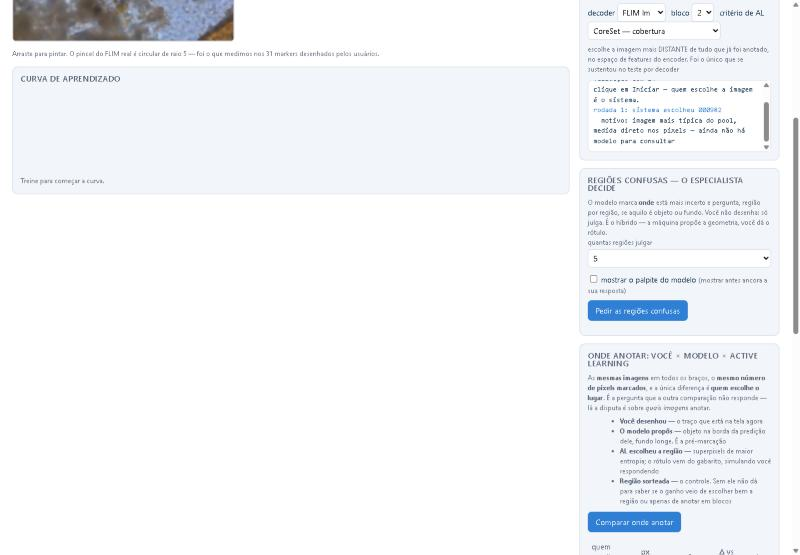
\includegraphics[width=0.62\linewidth]{plataforma_onde_anotar.jpg}
\caption[Comparação de onde anotar, na plataforma]{A comparação de posição de anotação. As mesmas imagens, o mesmo orçamento de pixels, e quatro formas de decidir onde o traço cai. O braço de região sorteada é o controle.}
\label{fig_plat_onde}
\end{figure}

\subsection{O que a tela registra}

Além da máscara corrente, a aplicação mantém a curva de qualidade por clique e três indicadores: a qualidade inicial, a melhor qualidade alcançada, e o número de cliques que \emph{pioraram} o resultado. O último indicador é o motivo de a tela existir. Com plasticidade máxima, que corresponde ao comportamento original, ele cresce ao longo da sessão, e o especialista observa diretamente o fenômeno descrito na Seção \ref{sec_cl_flim}: anotar mais não implica melhorar.

\subsection{Limite de uso dos números da aplicação}

A qualidade exibida na tela é calculada contra a anotação de referência do conjunto de dados, que existe porque se trata de ambiente de demonstração. Em uso real não haveria essa referência, e o especialista julgaria pela própria máscara.

A aplicação traz ainda um guia de anotação, reproduzido na Figura~\ref{fig_plat_tutorial}, que mostra lado a lado três formas de gastar a mesma quantidade de tinta na mesma imagem. Ele existe porque a orientação de onde tocar é contraintuitiva: a tendência natural de quem anota é preencher o centro do objeto, e o guia mostra o traço encostado no contorno.

\begin{figure}[htb]
\centering
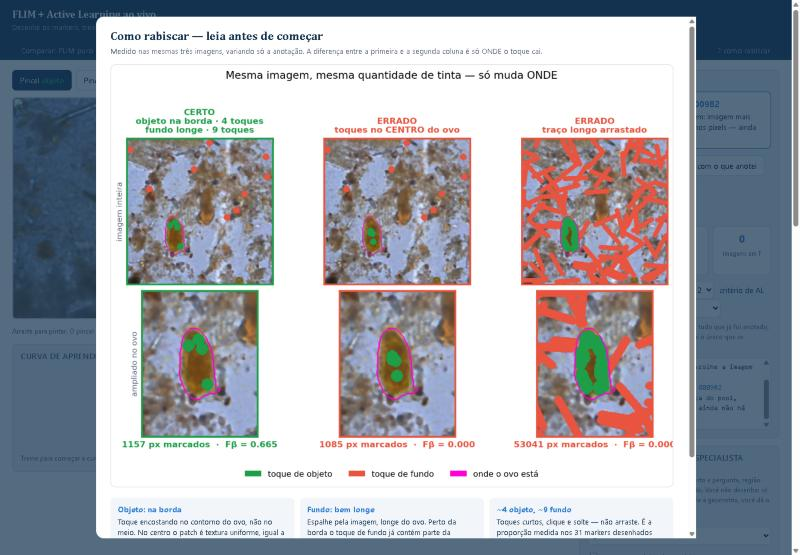
\includegraphics[width=\linewidth]{plataforma_tutorial.jpg}
\caption[Guia de anotação da plataforma]{O guia de anotação da aplicação. Mesma imagem e quantidade de pixels comparável nas três colunas; o que muda é a posição do traço. \textbf{Os valores de $F_\beta$ mostrados são ilustrativos e não constituem evidência}: vêm de uma execução única sobre três imagens, sem repetição por semente e sem teste pareado. A evidência sobre posição de anotação está no Capítulo~\ref{cap_4}.}
\label{fig_plat_tutorial}
\end{figure}

\textbf{Nenhum número produzido pela aplicação é usado nesta dissertação.} Ela roda com orçamento pequeno e execução única, regime em que a amplitude do braço de sorteio, entre 0,10 e 0,22 de $F_\beta$, é maior do que qualquer efeito que se queira observar. A aplicação serve para tornar o fenômeno visível e para permitir que um especialista opere o laço, não para medir. Todas as medições citadas vêm das campanhas em lote registradas no Capítulo~\ref{cap_4}.

Os valores apresentados pela aplicação não são usados em nenhuma afirmação desta dissertação. Eles vêm de execução única, sem repetição e sem controle de partição, e servem para inspeção qualitativa. Todas as medições relatadas no Capítulo \ref{cap_4} vêm das campanhas em lote, com semente, partição e registro.

\section{Protocolo experimental}

\subsection{Partições}

Cada conjunto de dados é dividido em três partes disjuntas: um conjunto de onde saem as imagens a anotar, um conjunto de validação usado nas medições de diagnóstico, e um conjunto de teste. A divisão é feita uma vez, com semente fixa, e mantida em todas as campanhas, de modo que resultados de campanhas diferentes sejam comparáveis.

O conjunto de teste não participou de nenhuma decisão de método: nenhum hiperparâmetro, critério, limiar ou faixa do filtro de área foi escolhido com base nele. Convém, porém, ser preciso sobre o que isso significa e o que não significa.

As campanhas de diagnóstico, que são as que sustentam os resultados centrais deste trabalho, medem \textbf{exclusivamente em validação}. É o caso do ganho marginal, da caracterização do comportamento dos critérios, da troca do gerador de candidatos e da análise de custo do aprendizado ativo.

A campanha de seleção de imagens, por outro lado, reporta desempenho \textbf{no conjunto de teste} para todos os braços, o que corresponde a cinco critérios, quatro orçamentos e três conjuntos de dados. Todos esses braços foram declarados antes da execução, de modo que se trata de reporte de configurações pré-especificadas e não de busca sobre o teste. Ainda assim, dizer que o conjunto de teste foi \emph{tocado uma única vez} seria impreciso, e essa formulação não é usada aqui.

\subsection{Repetições e unidade de análise}

Cada condição é repetida com dez sementes. Uma semente determina quais imagens são sorteadas para anotação e quais traços são gerados sobre elas, mantendo fixos a partição e o conjunto de validação.

A unidade independente de análise é a semente. Quando a mesma condição é avaliada com mais de um decodificador, os decodificadores de uma mesma semente compartilham o codificador e não constituem observações independentes; eles são colapsados por média antes de qualquer teste. Tratá-los como independentes multiplicaria artificialmente o tamanho amostral.

A consequência dessa escolha merece registro explícito: os intervalos de confiança descrevem a variação sob sorteio das imagens de treino \emph{naquele} conjunto de validação, e não generalizam para o conjunto de dados como um todo.

\subsection{Testes estatísticos}

As comparações são pareadas. Dentro de cada célula, os braços compartilham a partição, as imagens e os traços, de modo que a diferença entre eles isola o tratamento. Usa-se o teste $t$ pareado bicaudal, com nível de significância de $0{,}05$.

Quando uma campanha produz múltiplas comparações, aplica-se a correção de Benjamini-Hochberg sobre a família de testes, e o número de comparações que sobrevivem é reportado junto com os valores não corrigidos.

Resultados sobre proporções, como a taxa de sucesso do laço interativo, usam o teste exato de McNemar sobre os pares discordantes, já que pares concordantes não carregam informação sobre a diferença entre os braços.

\subsection{Pré-especificação versionada}
\label{sec_prereg}

Cada campanha é precedida de um documento que declara, antes da execução: a hipótese, o desfecho primário, os desfechos secundários, o critério que falsearia a hipótese, o número de repetições, e o que o experimento não autorizará afirmar.

O documento é versionado no mesmo repositório do código, e a ordem entre a declaração e a execução fica registrada nos \emph{commits}. Trata-se, portanto, de \textbf{pré-especificação versionada internamente}, e não de registro em plataforma externa e imutável como as usadas em ensaios clínicos ou em psicologia experimental. A distinção importa: um repositório sob controle do próprio autor oferece garantia mais fraca que um registro externo, ainda que o histórico torne a reescrita detectável. O que o procedimento garante é que a hipótese e o critério de falseamento existiam, em arquivo datado, antes de o resultado ser conhecido.

Essa disciplina tem motivo prático. Em um espaço com muitos critérios, conjuntos de dados e orçamentos, encontrar uma combinação aparentemente favorável é quase certo mesmo quando nenhum efeito existe. Declarar antes o que contaria como evidência é o que distingue um achado de um acidente. Quatro resultados aparentemente favoráveis foram descartados por esse procedimento ao longo deste trabalho, conforme relatado no Capítulo \ref{cap_4}.

Análises não previstas no pré-registro são permitidas e reportadas, mas identificadas como exploratórias, e qualquer afirmação derivada delas exige confirmação em repetições inéditas.

\subsection{Procedência dos resultados}

Toda execução avaliada é gravada em um registro único, com uma linha por execução, contendo a configuração, a semente, as imagens usadas, as métricas obtidas e o identificador do commit que produziu o resultado. O identificador de cada execução é derivado dos campos que a definem, de modo que reexecutar a mesma configuração produz o mesmo identificador e a duplicata se torna detectável.

As tabelas desta dissertação são geradas a partir desse registro por um programa, sem etapa manual. Cada tabela gerada acompanha um arquivo que lista os identificadores das execuções que produziram cada linha, o que torna a pergunta sobre a origem de um número respondível de forma direta.

\subsection{Reprodutibilidade numérica}

A estimação dos filtros envolve agrupamento por $k$-médias, cuja implementação recorre a bibliotecas de álgebra linear que distribuem o cálculo em várias linhas de execução. A ordem em que as somas parciais são reduzidas varia entre execuções, o que altera o resultado no último dígito representável.

No regime em que o agrupamento não ocorre, descrito pela Equação \ref{eq_regimes}, essa variação não tem efeito. No regime em que ocorre, ela é suficiente para que o agrupamento convirja para uma partição diferente, e o efeito se amplifica entre camadas, já que cada camada recebe como entrada as ativações da anterior.

Todas as campanhas são executadas com as bibliotecas limitadas a uma única linha de execução, condição sob a qual duas execuções idênticas produzem resultados idênticos. A verificação desse comportamento é relatada no Capítulo \ref{cap_4}.

\section{Materiais}

\subsection{Conjuntos de dados}

Três conjuntos são usados, escolhidos por apresentarem propriedades distintas quanto ao tamanho relativo do objeto, que a investigação mostrou ser determinante.

O conjunto de \textbf{parasitas} contém imagens de microscopia de ovos de \textit{Schistosoma mansoni}, em cores, com resolução de $400 \times 400$ pixels. O objeto ocupa cerca de 3\% da imagem. Estão disponíveis marcadores desenhados por dois especialistas, usados nas comparações que envolvem anotação real.

O conjunto \textbf{BraTS} \cite{menze2014multimodal} contém cortes de ressonância magnética cerebral, em tons de cinza, com resolução de $240 \times 240$ pixels.

O conjunto de \textbf{conjuntivite} contém fotografias oculares em cores e alta resolução, nas quais o objeto ocupa fração bem maior da imagem, com área mediana de aproximadamente 89 mil pixels.

A Figura~\ref{fig_datasets} mostra um exemplo de cada um, com a anotação de referência sobreposta e a máscara isolada. Três propriedades ficam visíveis de imediato e sustentam leituras feitas adiante: os três são de segmentação \emph{binária}, e não multiclasse; o objeto ocupa fração pequena da imagem em dois deles, o que é a razão de a acurácia passar de 0,97 em quase todas as configurações sem distinguir braço nenhum; e os domínios são visualmente muito distintos entre si, o que é precisamente o que torna informativo um método falhar nos três.

\begin{figure}[htb]
\centering
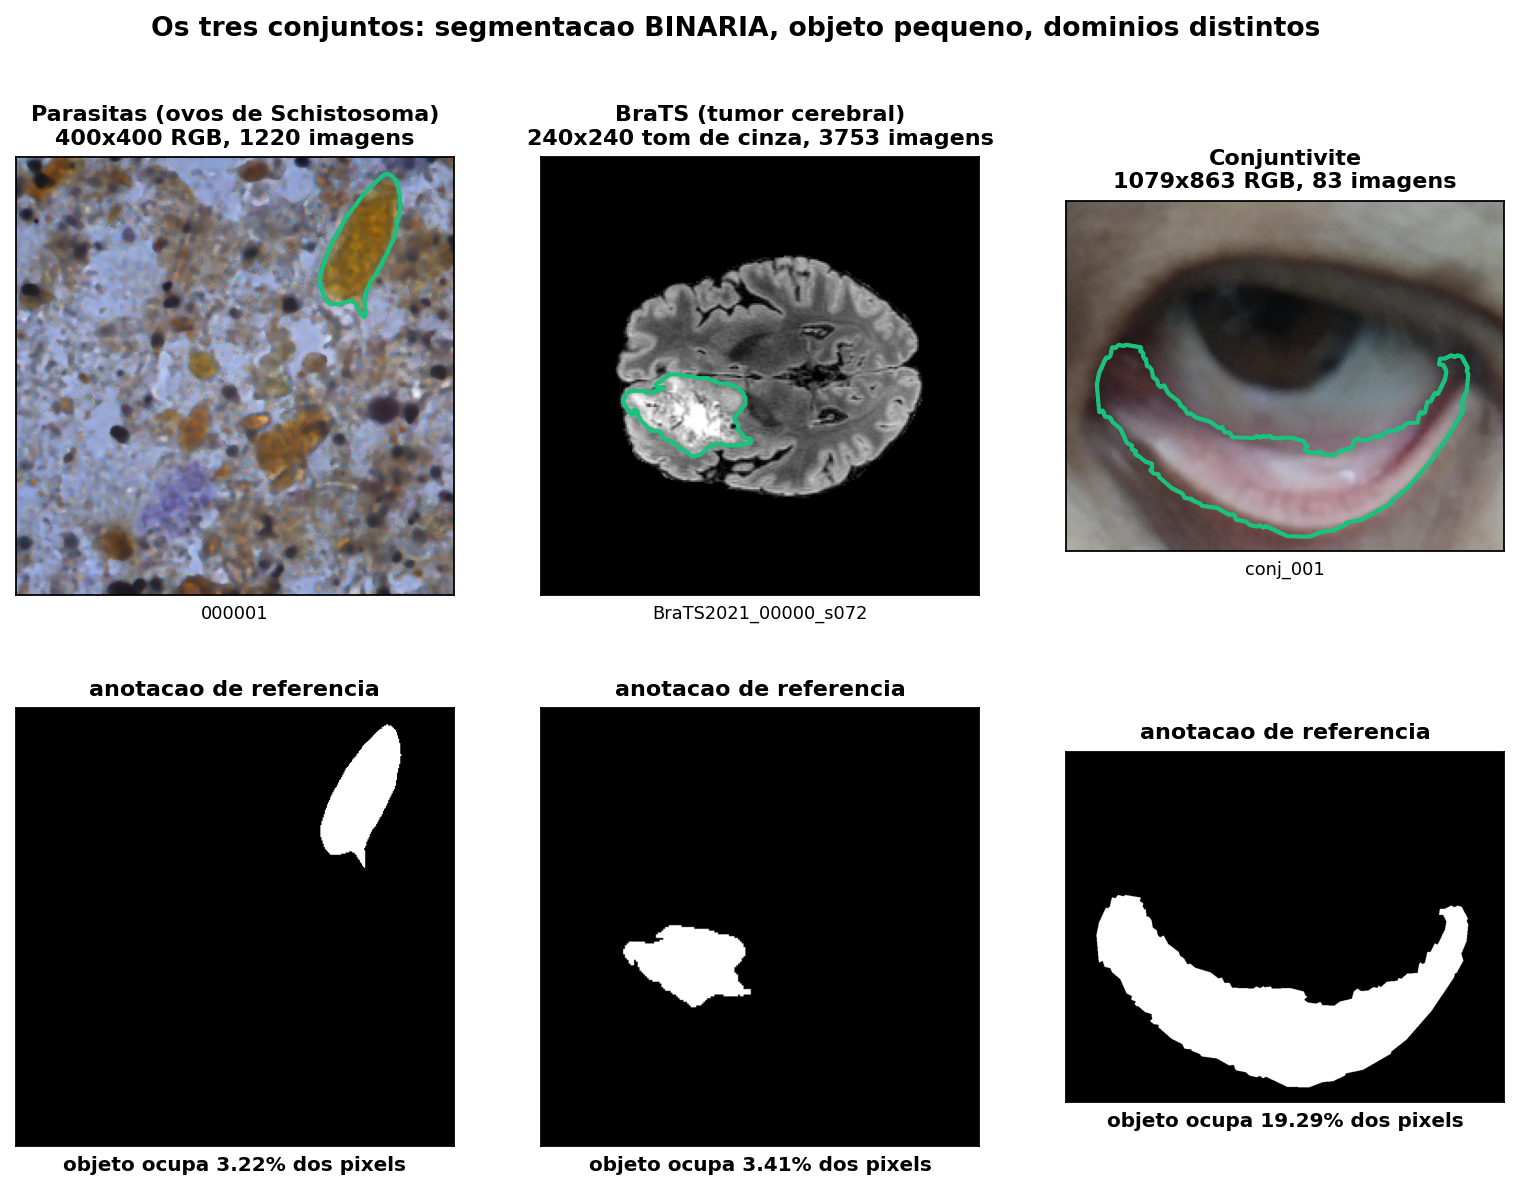
\includegraphics[width=\linewidth]{datasets.png}
\caption[Os três conjuntos de dados usados nos experimentos]{Um exemplo de cada conjunto, com a anotação de referência em verde na linha superior e a máscara isolada na linha inferior. A fração de pixels de objeto indicada em cada painel é medida na máscara do exemplo mostrado.}
\label{fig_datasets}
\end{figure}

\subsection{Levantamento de domínios candidatos}

A escolha dos três conjuntos acima partiu de um levantamento mais amplo de domínios em que a segmentação interativa reduziria esforço de anotação de forma significativa. O critério de seleção considerou a diversidade de desafios que cada domínio impõe, e não apenas a disponibilidade dos dados.

Em gastroenterologia e dermatologia, o Kvasir-SEG \cite{jha2020kvasir} apresenta bordas irregulares de pólipos e artefatos de iluminação, enquanto o ISIC 2018 \cite{codella2018skin} caracteriza-se por alta variabilidade de cor e textura da pele, com interferência de sombras, presença de pelos e heterogeneidade entre pacientes.

Em radiologia e oncologia, o BraTS \cite{menze2014multimodal} e o LiTS \cite{bilic2019liver} introduzem modalidades volumétricas processadas em fatias bidimensionais, com canais monocromáticos e contraste baixo entre tecidos.

Em ultrassonografia e oftalmologia, o BUSI \cite{al2020dataset} impõe ruído característico da modalidade, e o REFUGE2 \cite{fang2022refuge2} exige definição anatômica precisa de estruturas oculares.

A Figura~\ref{fig_dominios} reúne exemplos desses domínios. A diversidade de modalidade é evidente, e é justamente ela que torna o levantamento inicial plausível: endoscopia, dermatoscopia, ressonância, tomografia e ultrassonografia impõem desafios de aparência muito diferentes.

\begin{figure}[htb]
\centering
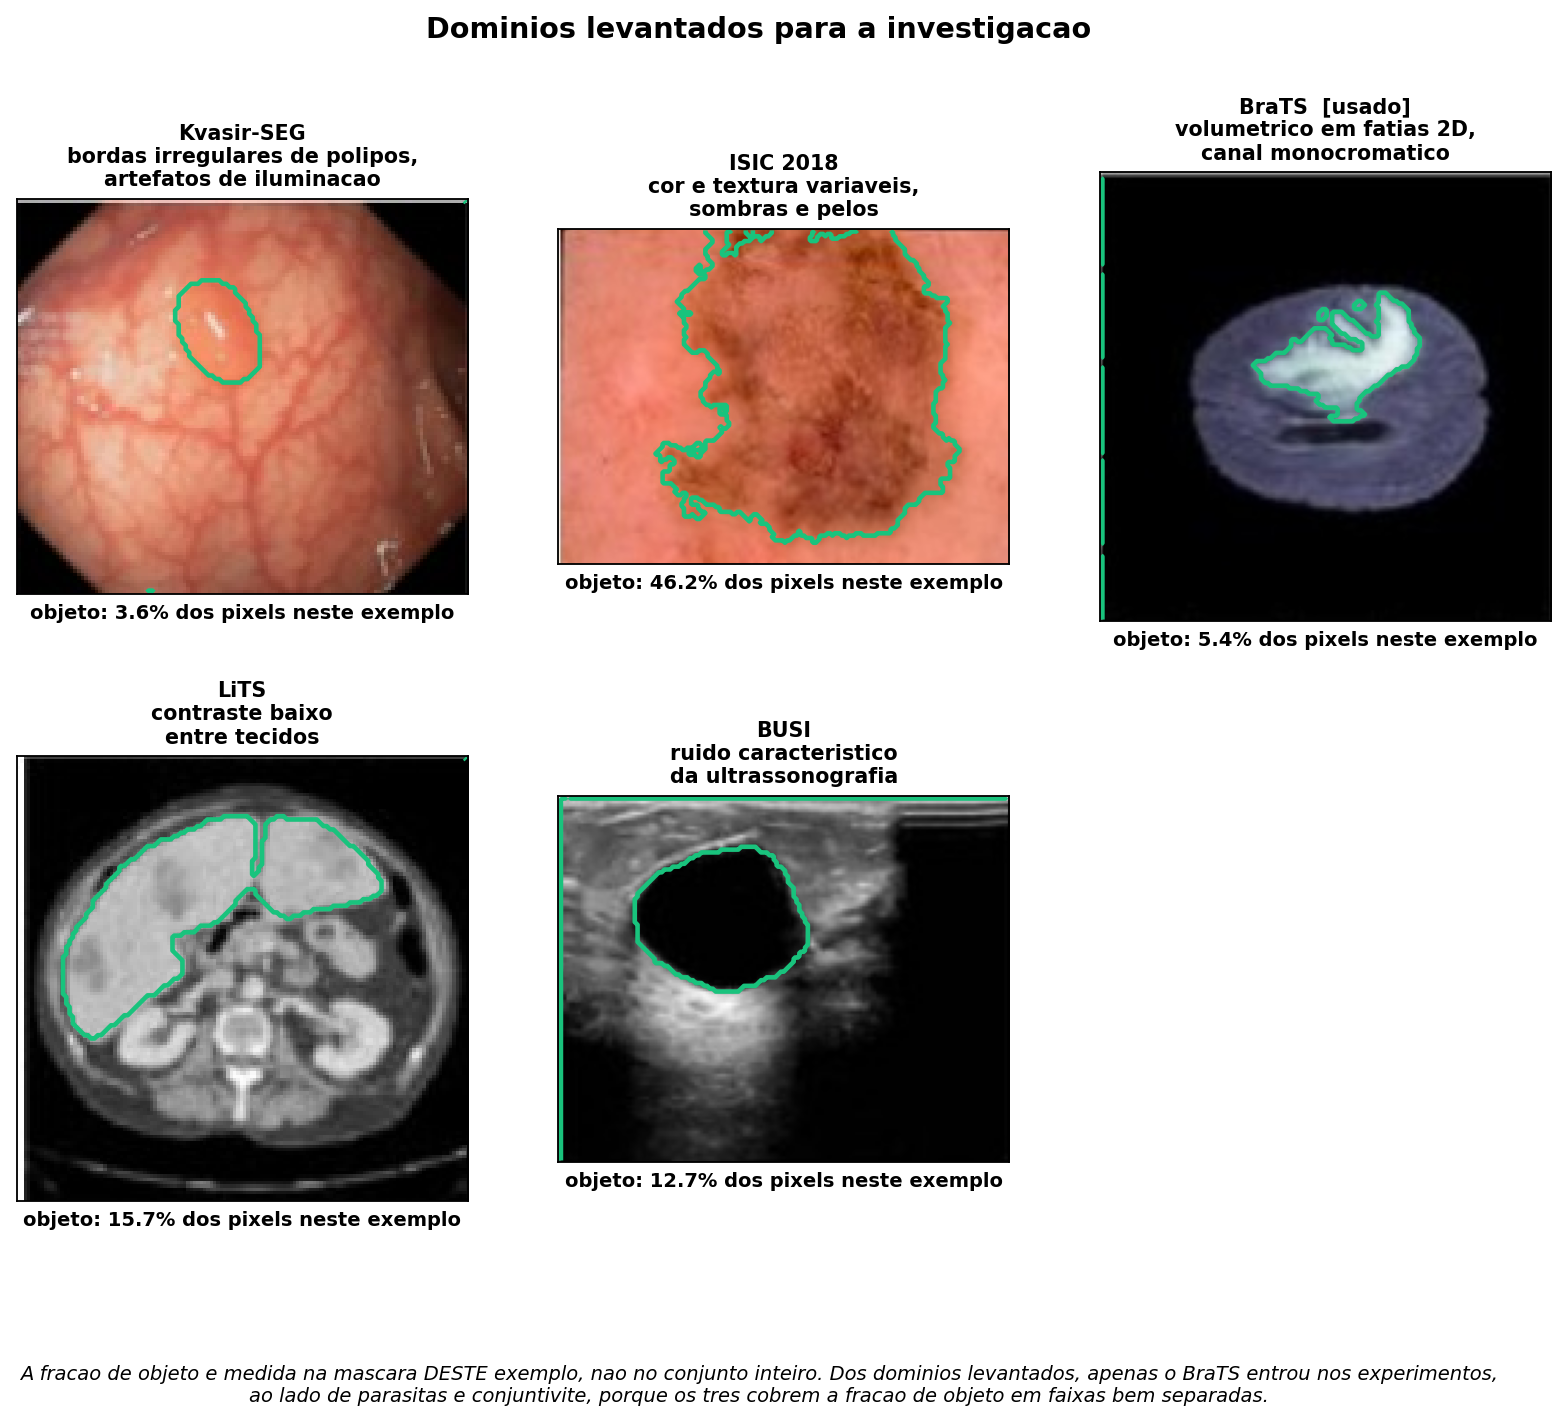
\includegraphics[width=\linewidth]{dominios_levantados.png}
\caption[Exemplos dos domínios levantados]{Exemplos dos domínios considerados no levantamento, com a anotação de referência sobreposta. A fração de objeto indicada é medida na máscara do exemplo mostrado e não é estatística do conjunto. O REFUGE2, citado no texto, não aparece porque o par de imagem e máscara disponível no repositório não corresponde entre si.}
\label{fig_dominios}
\end{figure}

Dos domínios levantados, três foram efetivamente usados nos experimentos. A razão é que a investigação revelou, ao longo do trabalho, que a propriedade determinante para o comportamento dos métodos avaliados não é a modalidade de aquisição, e sim a \emph{fração da imagem ocupada pelo objeto}, que controla a razão entre candidatos a filtro e canais disponíveis descrita na Equação \ref{eq_regimes}. Os três conjuntos escolhidos cobrem essa propriedade em faixas bem separadas, de cerca de 3\% a mais de 20\%, o que se mostrou mais informativo do que acrescentar domínios com fração semelhante.

\subsection{Modelos de comparação}

Além do \ac{FLIM} com decodificador adaptativo, foram treinados cinco modelos de referência para contextualizar os valores obtidos: SAMNet, MSCNet, MEANet, UNet e uma variante UNet com codificador \ac{FLIM}. Esses modelos são treinados por retropropagação e com conjuntos anotados completos, de modo que não constituem comparação direta quanto ao esforço de anotação; servem para situar a ordem de grandeza da qualidade atingível em cada domínio.

\subsection{Ambiente}

Os experimentos foram executados em ambiente nativo, com a biblioteca de agrupamento do \textit{scikit-learn}. Uma implementação alternativa de $k$-médias, mais rápida, está disponível na biblioteca original mas não foi utilizada, porque produz centróides diferentes e portanto filtros diferentes, o que tornaria os resultados incomparáveis entre si.

A avaliação não emprega o delineamento por árvores dinâmicas descrito no trabalho de referência, por indisponibilidade do executável na plataforma utilizada. Em seu lugar, usa-se limiarização de Otsu seguida de filtro de área, conforme descrito na Seção \ref{sec_decoder}. Os valores reproduzidos, portanto, não são diretamente comparáveis aos publicados, e essa limitação acompanha toda comparação com o trabalho original.

\chapter{Resultados}\label{cap_4}

Este capítulo apresenta os resultados em uma ordem que acompanha o raciocínio da investigação, e não a cronologia dos experimentos. Primeiro a reprodução do trabalho de referência, que define o ponto de partida. Depois a avaliação dos critérios de \ac{AL} sobre a seleção de imagens, que é a forma usual de aplicar a técnica. Em seguida o diagnóstico que mede quanta margem existe na escolha da região, e a caracterização de para onde cada critério aponta, que juntos explicam por que os critérios conhecidos não alcançam essa margem. Os componentes de \ac{CL} e \ac{IL} vêm na sequência. O capítulo fecha com a intervenção derivada do diagnóstico e com os resultados de natureza metodológica.

Todos os números vêm do registro de execuções descrito no Capítulo \ref{cap_3}. Cada tabela é gerada a partir desse registro por um programa, sem passo manual, e acompanha um arquivo de procedência que lista os identificadores das execuções que produziram cada linha. Nenhum valor foi transcrito à mão.

\section{Reprodução do trabalho de referência}

A reprodução do arranjo descrito por \cite{soares2026flim} confirma o comportamento central relatado pelos autores: o $F_\beta$ cresce de forma monotônica à medida que imagens são acrescentadas ao conjunto de treino e satura entre três e quatro imagens, atingindo valores próximos aos publicados para o codificador.

Duas diferenças de implementação precisam ser declaradas antes de qualquer comparação numérica. A primeira é que a avaliação usa limiarização de Otsu seguida de filtro de área, e não o delineamento por árvores dinâmicas empregado no trabalho original, cujo executável é um binário compilado para Linux que não roda no ambiente usado aqui. A segunda é que a seleção de imagens do Algoritmo 1 do trabalho de referência exige o ground truth de todo o conjunto disponível para escolher as poucas imagens que serão anotadas, o que os próprios autores declaram ao descrever a abordagem como supervisionada.

Essa segunda diferença não é um detalhe de implementação, e sim o ponto de partida desta dissertação. Se a escolha das imagens depende de conhecer a resposta em todas elas, o procedimento não é aplicável na situação que motiva o \ac{FLIM}, que é justamente a ausência de anotação. A pergunta que organiza os experimentos seguintes é quanto do benefício dessa escolha se recupera com critérios que não usam ground truth algum.

A Figura~\ref{fig_curva} e a Tabela~\ref{tab_curva} mostram o comportamento da curva de orçamento. A saturação entre três e quatro imagens é o que responde à pergunta de por que o trabalho de referência usa esse número: o algoritmo para quando acrescentar imagem deixa de melhorar o $F_\beta$.

\begin{figure}[htb]
\centering
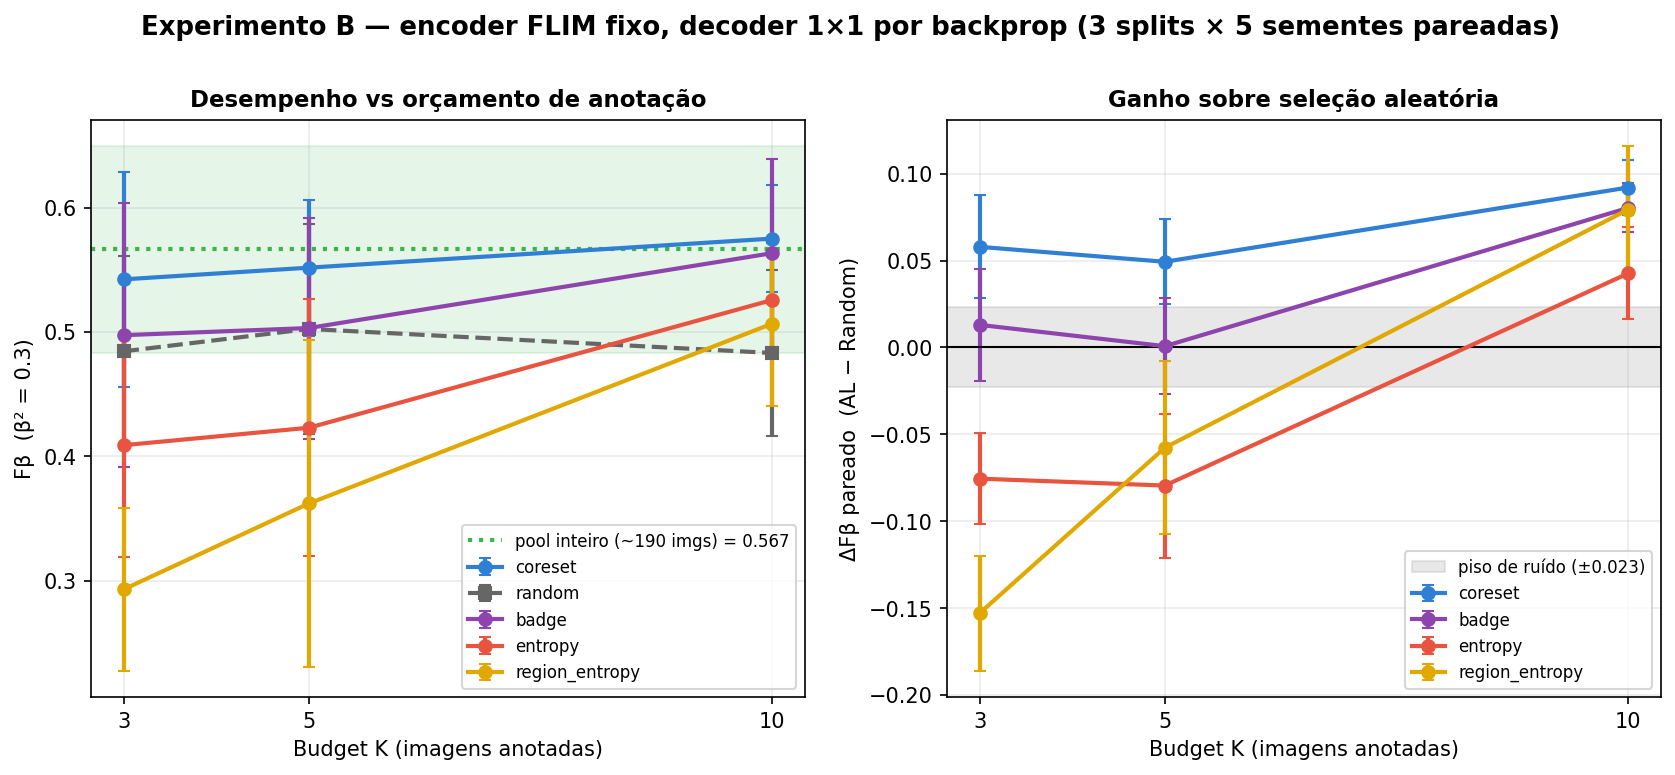
\includegraphics[width=0.86\linewidth]{curva_orcamento.png}
\caption[Qualidade em função do número de imagens anotadas]{Qualidade em função do número de imagens anotadas, com a faixa de ruído da reexecução. A curva satura entre três e quatro imagens, e o ganho posterior cabe dentro do intervalo de confiança.}
\label{fig_curva}
\end{figure}

\begin{table}[htb]
\centering
\caption{Qualidade por número de imagens anotadas.}
\label{tab_curva}
% Fβ por número de imagens anotadas
% GERADO por flim_al/tabelas.py em 2026-10-08T14:01:05+00:00
% NAO EDITE A MAO: a proxima geracao sobrescreve, e o numero editado deixa de bater com evidencia/execucoes/.
% Proveniencia: curva_orcamento.proveniencia.json
\begin{tabular}{lrrrrr}
\toprule
imagens & F$\beta$ médio & desvio & IC95\% & n & seeds \\
\midrule
1 & 0.602 & 0.084 & [0.580, 0.625] & 54 & 9 \\
2 & 0.576 & 0.143 & [0.538, 0.615] & 54 & 9 \\
3 & 0.645 & 0.074 & [0.625, 0.664] & 57 & 9 \\
4 & 0.670 & 0.077 & [0.650, 0.691] & 54 & 9 \\
5 & 0.665 & 0.093 & [0.642, 0.688] & 63 & 9 \\
6 & 0.645 & 0.104 & [0.619, 0.672] & 58 & 9 \\
7 & 0.680 & 0.080 & [0.659, 0.701] & 54 & 9 \\
8 & 0.676 & 0.085 & [0.656, 0.697] & 65 & 9 \\
9 & 0.686 & 0.063 & [0.671, 0.702] & 64 & 9 \\
10 & 0.599 & 0.111 & [0.554, 0.644] & 26 & 5 \\
12 & 0.767 & 0.000 & [0.767, 0.767] & 3 & 0 \\
16 & 0.781 & 0.002 & [0.778, 0.785] & 3 & 0 \\
20 & 0.772 & 0.001 & [0.771, 0.773] & 3 & 0 \\
25 & 0.759 & 0.006 & [0.743, 0.775] & 3 & 0 \\
31 & 0.711 & 0.000 & [0.711, 0.711] & 3 & 0 \\
\bottomrule
\end{tabular}

\end{table}

% Nota de curva_orcamento. GERADA por flim_al/tabelas.py.
\footnotesize Seleção sem consulta ao gabarito. \texttt{n} conta execuções; \texttt{seeds} conta sementes distintas --- nove execuções de uma semente só não são nove repetições.
\normalsize


Uma ressalva importante acompanha essa leitura, e ela diz respeito ao que a curva mistura. A arquitetura pede duzentos núcleos por camada, mas o agrupamento só produz tantos quantos os trechos sob os marcadores permitem. Com uma imagem anotada o codificador sai com 54, 51, 48 e 48 núcleos nas quatro camadas; com oito, sai com duzentos em todas. Com pouca anotação a rede não é apenas menos treinada, \textbf{ela é menor}. Parte do ganho que a curva mostra nos primeiros pontos é, portanto, aumento de capacidade, e não aumento de supervisão, e separar as duas contribuições exigiria fixar o tamanho do codificador ao longo da curva.

Nas cinco últimas linhas da Tabela~\ref{tab_curva}, referentes a doze imagens ou mais, a coluna de sementes distintas indica zero. Isso significa que o registro não guardou semente distinta para essas execuções, de modo que três execuções de uma mesma semente não constituem três repetições, e o desvio nulo é artefato disso, não estabilidade.

A reimplementação do Algoritmo 1 revelou ainda duas propriedades não discutidas no trabalho original. O critério de selecionar a imagem de pior $F_\beta$ tende a escolher imagens insegmentáveis, e não imagens informativas: as imagens com $F_\beta$ igual a zero são aquelas cujas componentes previstas caem fora da faixa aceita pelo filtro de área, de modo que o algoritmo prioriza casos em que nenhuma anotação ajudaria. Além disso, sem uma lista de imagens rejeitadas, a imagem removida pelo retrocesso volta a ser a de menor $F_\beta$ na iteração seguinte, e o procedimento pode entrar em ciclo.

\section{Seleção de imagens}

A primeira pergunta é se algum critério de \ac{AL} sem ground truth supera a escolha aleatória das imagens a anotar. Foram avaliados critérios das duas famílias predominantes na literatura: incerteza, representada por entropia, \textit{least confidence}, margem e BALD; e diversidade, representada por CoreSet, BADGE e medoide. A referência superior é o oracle, que usa o ground truth para escolher a imagem de pior desempenho, e a referência inferior é o sorteio.

A Tabela \ref{tab_geral_al} resume a comparação nos três conjuntos de dados, para quatro orçamentos de anotação.

\begin{table}[htb]
\centering
\caption{Critérios de Active Learning por orçamento e conjunto de dados.}
\label{tab_geral_al}
% Active Learning no FLIM: todos os critérios, todos os K (FLIM_lm)
% GERADO por flim_al/tabelas.py em 2026-10-06T16:49:56+00:00
% NAO EDITE A MAO: a proxima geracao sobrescreve, e o numero editado deixa de bater com evidencia/execucoes/.
% Proveniencia: geral_al_lm.proveniencia.json
\begin{tabular}{llrrrrrr}
\hline
critério & K & Parasitas & BraTS & Conjuntivite & $\Delta$ médio vs sorteio & p & vence o sorteio em \\
\hline
CoreSet (imagem) & 2 & 0.543 & 0.000 & 0.642 & -0.061 & 0.5568 & 3 de 9 \\
CoreSet (imagem) & 3 & 0.538 & 0.033 & 0.587 & 0.023 & 0.6074 & 3 de 9 \\
CoreSet (imagem) & 5 & 0.640 & 0.489 & 0.748 & 0.112 & 0.3323 & 7 de 9 \\
CoreSet (imagem) & 8 & 0.690 & 0.230 & 0.636 & -0.067 & 0.4144 & 3 de 9 \\
Entropia (imagem) & 2 & 0.457 & 0.001 & 0.635 & -0.092 & 0.3677 & 3 de 9 \\
Entropia (imagem) & 3 & 0.474 & 0.000 & 0.591 & -0.008 & 0.9104 & 2 de 9 \\
Entropia (imagem) & 5 & 0.599 & 0.498 & 0.667 & 0.074 & 0.5274 & 6 de 9 \\
Entropia (imagem) & 8 & 0.681 & 0.000 & 0.604 & -0.157 & 0.0427 & 2 de 9 \\
Least confidence (imagem) & 2 & 0.420 & 0.001 & 0.635 & -0.105 & 0.3115 & 3 de 9 \\
Least confidence (imagem) & 3 & 0.451 & 0.000 & 0.591 & -0.016 & 0.8178 & 2 de 9 \\
Least confidence (imagem) & 5 & 0.583 & 0.498 & 0.667 & 0.069 & 0.5531 & 6 de 9 \\
Least confidence (imagem) & 8 & 0.684 & 0.000 & 0.441 & -0.210 & 0.0327 & 2 de 9 \\
AL de REGIAO & 2 & 0.142 & 0.252 & 0.442 & -0.178 & 0.2461 & 1 de 9 \\
AL de REGIAO & 3 & 0.280 & 0.257 & 0.443 & -0.036 & 0.7332 & 3 de 9 \\
AL de REGIAO & 5 & 0.039 & 0.499 & 0.261 & -0.247 & 0.1570 & 2 de 9 \\
AL de REGIAO & 8 & 0.412 & 0.525 & 0.308 & -0.170 & 0.1903 & 2 de 9 \\
Oracle (usa GT) & 2 & 0.093 & 0.196 & 0.274 & -0.269 & 0.0921 & 1 de 9 \\
Oracle (usa GT) & 3 & 0.420 & 0.630 & 0.312 & 0.091 & 0.5347 & 5 de 9 \\
Oracle (usa GT) & 5 & 0.618 & 0.445 & 0.572 & 0.031 & 0.7792 & 6 de 9 \\
Oracle (usa GT) & 8 & 0.518 & 0.008 & 0.535 & -0.232 & 0.0107 & 0 de 9 \\
\hline
\end{tabular}

\end{table}

% Nota de geral_al_lm. GERADA por flim_al/tabelas.py.
\footnotesize Uma linha por (critério, K). As colunas de dataset são o F$\beta$ médio sobre as sementes. \textbf{\texttt{FLIM puro (sorteio)} é a referência}: todos os braços recebem o MESMO número de imagens e são medidos no mesmo conjunto de teste. Os critérios de IMAGEM escolhem quais imagens anotar; \textbf{\texttt{AL de REGIÃO} usa as mesmas imagens do sorteio e muda só ONDE o traço cai}, com a mesma contagem de pixels --- o $\Delta$ dele mede posição de anotação, não escolha de imagem. \textbf{\texttt{Oracle} usa o gabarito} para escolher a imagem em que o modelo vai pior (passo 7 do Algoritmo 1 do artigo): não é método, é referência, e o fato de ele também não se destacar é o achado mais informativo daqui. $\Delta$ e p são pareados por semente dentro de cada dataset e K, depois agregados. \texttt{vence o sorteio em} conta as células (dataset $\times$ semente) favoráveis. Decoder FLIM\_lm.
\normalsize


Nenhum critério apresenta superioridade sobre o sorteio que sobreviva à correção de Benjamini-Hochberg. O resultado se mantém nos três conjuntos de dados e nos quatro orçamentos. Vale notar que o oracle, que lê o ground truth e portanto representa o teto do que a seleção de imagens poderia entregar, também não se destaca de forma consistente, perdendo do sorteio em parte considerável das células. Isso sugere que, no regime de três a cinco imagens, a identidade das imagens escolhidas importa menos do que a formulação do Algoritmo 1 pressupõe.

É importante enunciar esse resultado com precisão. O que foi observado é ausência de evidência de superioridade nas condições avaliadas, e não demonstração de equivalência. Os intervalos de confiança são compatíveis com efeitos pequenos em qualquer direção, e o número de repetições limita o tamanho de efeito detectável.

A Tabela~\ref{tab_comparacao_criterios} apresenta o conjunto completo de técnicas que chegaram a rodar, incluindo as que perderam do sorteio. Ela é deliberadamente exaustiva: apresentar apenas as técnicas que se saíram melhor seria seleção de resultado, e a leitura correta deste capítulo depende de ver que o fenômeno é geral e não um acidente de uma implementação.

\begin{table}[htb]
\centering
\caption{Todas as técnicas avaliadas, contra o sorteio.}
\label{tab_comparacao_criterios}
% Técnicas de Active Learning contra o sorteio
% GERADO por flim_al/tabelas.py em 2026-10-08T14:01:04+00:00
% NAO EDITE A MAO: a proxima geracao sobrescreve, e o numero editado deixa de bater com evidencia/execucoes/.
% Proveniencia: comparacao_criterios.proveniencia.json
\begin{adjustbox}{max width=\linewidth}
\begin{tabular}{lrrrrrrrrr}
\toprule
técnica & nível & F$\beta$ (células pareadas) & n pares & $\Delta$ vs random & p & $\Delta$ vs FLIM (K=3) & p (FLIM) & $\Delta$ vs controle do nível & veredito \\
\midrule
badge & imagem & 0.430 & 95 & \textbf{-0.019} & 0.0105 & --- & --- & --- & suportado \\
coreset & imagem & 0.464 & 354 & \textbf{-0.028} & 0.0149 & --- & --- & --- & suportado \\
entropy & imagem & 0.455 & 471 & -0.009 & 0.3661 & --- & --- & --- & sem suporte \\
least\_confidence & imagem & 0.437 & 369 & -0.020 & 0.0937 & --- & --- & --- & indicativo \\
margin & imagem & 0.451 & 72 & 0.023 & 0.2110 & --- & --- & --- & sem suporte \\
random & imagem & --- & --- & --- & --- & --- & --- & --- & piso \\
oracle & imagem (usa GT) & 0.514 & 103 & -0.020 & 0.4456 & --- & --- & --- & sem suporte \\
flim\_3img & linha de base & --- & 0 & --- & --- & --- & --- & --- & sem pares suficientes \\
random\_region & região & 0.442 & 252 & \textbf{0.108} & 0.0000 & --- & --- & --- & suportado \\
region\_bald & região & 0.462 & 135 & \textbf{0.077} & 0.0000 & --- & --- & 0.050 & suportado \\
region\_entropy & região & 0.437 & 66 & 0.014 & 0.4295 & --- & --- & --- & sem suporte \\
1\_imagens & ? & --- & 0 & --- & --- & --- & --- & --- & sem pares suficientes \\
2\_imagens & ? & --- & 0 & --- & --- & --- & --- & --- & sem pares suficientes \\
3\_imagens & ? & --- & 0 & --- & --- & --- & --- & --- & sem pares suficientes \\
5\_imagens & ? & --- & 0 & --- & --- & --- & --- & --- & sem pares suficientes \\
8\_imagens & ? & --- & 0 & --- & --- & --- & --- & --- & sem pares suficientes \\
al\_regiao & ? & 0.456 & 28 & \textbf{-0.032} & 0.0439 & --- & --- & --- & suportado \\
aleatorio\_objeto & ? & --- & 0 & --- & --- & --- & --- & --- & sem pares suficientes \\
argmax\_entropia & ? & --- & 0 & --- & --- & --- & --- & --- & sem pares suficientes \\
argmax\_lc & ? & --- & 0 & --- & --- & --- & --- & --- & sem pares suficientes \\
argmax\_prob & ? & --- & 0 & --- & --- & --- & --- & --- & sem pares suficientes \\
artigo & ? & --- & 0 & --- & --- & --- & --- & --- & sem pares suficientes \\
base & ? & --- & 0 & --- & --- & --- & --- & --- & sem pares suficientes \\
contorno\_sorteado & ? & --- & 0 & --- & --- & --- & --- & --- & sem pares suficientes \\
flim\_paper & ? & 0.467 & 69 & -0.015 & 0.4074 & --- & --- & --- & sem suporte \\
flim\_puro & ? & --- & 0 & --- & --- & --- & --- & --- & sem pares suficientes \\
il\_alpha0.00 & ? & --- & 0 & --- & --- & --- & --- & --- & sem pares suficientes \\
il\_alpha0.50 & ? & --- & 0 & --- & --- & --- & --- & --- & sem pares suficientes \\
il\_alpha1.00 & ? & --- & 0 & --- & --- & --- & --- & --- & sem pares suficientes \\
imagem\_nova & ? & --- & 0 & --- & --- & --- & --- & --- & sem pares suficientes \\
medoide & ? & 0.482 & 94 & \textbf{-0.043} & 0.0054 & --- & --- & --- & suportado \\
melhor\_sorteada & ? & --- & 0 & --- & --- & --- & --- & --- & sem pares suficientes \\
pior\_sorteada & ? & --- & 0 & --- & --- & --- & --- & --- & sem pares suficientes \\
regiao\_aleatoria & ? & --- & 0 & --- & --- & --- & --- & --- & sem pares suficientes \\
regiao\_borda & ? & --- & 0 & --- & --- & --- & --- & --- & sem pares suficientes \\
regiao\_confusa & ? & 0.396 & 71 & -0.075 & 0.0766 & --- & --- & --- & indicativo \\
regiao\_incerteza & ? & --- & 0 & --- & --- & --- & --- & --- & sem pares suficientes \\
sorteada & ? & --- & 0 & --- & --- & --- & --- & --- & sem pares suficientes \\
sorteado & ? & --- & 0 & --- & --- & --- & --- & --- & sem pares suficientes \\
uniforme & ? & --- & 0 & --- & --- & --- & --- & --- & sem pares suficientes \\
uniforme\_balanceado & ? & --- & 0 & --- & --- & --- & --- & --- & sem pares suficientes \\
\bottomrule
\end{tabular}
\end{adjustbox}

\end{table}

% Nota de comparacao_criterios. GERADA por flim_al/tabelas.py.
\footnotesize \texttt{random} é o piso --- sem critério nenhum. O pareamento casa split, decoder, orçamento e semente \textbf{dentro da mesma família de experimento}; a média mostrada vem dessas mesmas células, para que média e $\Delta$ falem do mesmo conjunto. \textbf{Toda técnica que rodou está aqui, inclusive as que perderam do sorteio} --- no experimento de encoder retreinado isso aconteceu com as quatro de imagem. Negrito só com p < 0,05. Para técnicas de REGIÃO, leia a coluna do controle de nível (\texttt{random\_region}): o $\Delta$ contra \texttt{random} soma seleção e geometria, e a geometria pesa ~2$\times$ a seleção neste projeto. \textbf{\texttt{flim\_3img} é o FLIM do artigo} --- as 3 imagens que os autores escolheram, sem seleção automática. A coluna \texttt{$\Delta$ vs FLIM} responde à pergunta central: aplicar AL melhora sobre isso? Ela só aparece em orçamento casado (K=3), porque o braço do artigo só existe com 3 imagens; comparar AL com 10 imagens contra FLIM com 3 mediria orçamento, não seleção. \textbf{Coluna toda vazia significa comparação IMPOSSÍVEL com os dados existentes, não ausente por descuido}: o braço do artigo usa os 31 markers REAIS do especialista, e os braços de AL sobre o pool completo usam sintéticos, porque marker real só existe para 31 imagens. \texttt{marker\_origem} entra no pareamento para que esse par não se forme --- ele mediria quem desenhou o traço e apresentaria como efeito da seleção. Para responder à pergunta, rode \texttt{scripts/varrer\_criterios.py --modo imagem}: marker real nos dois lados, com \texttt{oracle} (o passo 7 do Algoritmo 1) como referência.
\normalsize


Linhas com células vazias merecem explicação, porque a ausência ali não é descuido. O braço do trabalho de referência usa os trinta e um conjuntos de marcadores \emph{reais} dos especialistas, enquanto os braços de \ac{AL} sobre o conjunto completo usam marcadores sintéticos, pela razão simples de que marcador real só existe para essas trinta e uma imagens. A origem do marcador entra no pareamento justamente para impedir que esse par se forme: se formasse, a diferença mediria quem desenhou o traço e seria apresentada como efeito da seleção. Onde a coluna aparece vazia, a comparação é \textbf{impossível} com os dados existentes.

A Tabela~\ref{tab_custo} traz o custo computacional medido, que é parte do argumento a favor do \ac{FLIM} e precisa ser registrado ao lado da qualidade. Estimar os núcleos por agrupamento leva de 0,8 segundo com uma imagem a 48,1 segundos com oito. O tempo de avaliação cresce com o orçamento pela razão já discutida: o codificador cresce junto. Todas as linhas vêm de uma única campanha com uma semente, de modo que servem para ordem de grandeza e não para comparar critérios entre si.

\begin{table}[htb]
\centering
\caption{Qualidade por critério e orçamento nos sete decodificadores, com custo.}
\label{tab_custo}
% Fβ por critério e orçamento, nos sete decoders, com custo
% GERADO por flim_al/tabelas.py em 2026-10-08T13:52:40+00:00
% NAO EDITE A MAO: a proxima geracao sobrescreve, e o numero editado deixa de bater com evidencia/execucoes/.
% Proveniencia: k_por_modelo.proveniencia.json
\begin{adjustbox}{max width=\linewidth}
\begin{tabular}{llrrrrrrrrrrrr}
\toprule
critério & K & n & FLIM\_lm & FLIM\_pb & FLIM\_mb & FLIM\_at & FLIM\_ts & FLIM\_lt & FLIM\_ts* & melhor & $\Delta$ vs artigo & treino (s) & teste (s) \\
\midrule
flim\_paper & 1 & 1 & 0.443 & 0.530 & 0.341 & 0.420 & 0.329 & 0.294 & 0.362 & 0.530 (FLIM\_pb) & 0.000 & 0.8 & 85.4 \\
flim\_paper & 2 & 1 & 0.433 & 0.574 & 0.417 & 0.299 & 0.460 & 0.409 & 0.273 & 0.574 (FLIM\_pb) & 0.000 & 2.4 & 125.8 \\
flim\_paper & 3 & 1 & 0.133 & 0.623 & 0.213 & 0.125 & 0.240 & 0.242 & 0.243 & 0.623 (FLIM\_pb) & 0.000 & 4.3 & 160.6 \\
flim\_paper & 4 & 1 & 0.575 & 0.634 & 0.418 & 0.196 & 0.488 & 0.610 & 0.403 & 0.634 (FLIM\_pb) & 0.000 & 7.9 & 210.4 \\
flim\_paper & 5 & 1 & 0.628 & 0.659 & 0.415 & 0.364 & 0.470 & 0.535 & 0.378 & 0.659 (FLIM\_pb) & 0.000 & 11.9 & 211.6 \\
coreset & 1 & 1 & 0.661 & 0.641 & 0.341 & 0.176 & 0.323 & 0.277 & 0.334 & 0.661 (FLIM\_lm) & 0.005 & 0.9 & 97.7 \\
coreset & 2 & 1 & 0.657 & 0.491 & 0.217 & 0.209 & 0.167 & 0.136 & 0.293 & 0.657 (FLIM\_lm) & -0.099 & 3.2 & 143.0 \\
coreset & 3 & 1 & 0.323 & 0.594 & 0.199 & 0.167 & 0.104 & 0.179 & 0.240 & 0.594 (FLIM\_pb) & -0.001 & 4.3 & 182.1 \\
coreset & 4 & 1 & 0.604 & 0.561 & 0.329 & 0.249 & 0.308 & 0.317 & 0.326 & 0.604 (FLIM\_lm) & -0.090 & 9.3 & 246.2 \\
coreset & 5 & 1 & 0.460 & 0.683 & 0.462 & 0.372 & 0.498 & 0.539 & 0.385 & 0.683 (FLIM\_pb) & -0.007 & 14.0 & 257.2 \\
coreset & 8 & 1 & 0.682 & 0.617 & 0.379 & 0.288 & 0.441 & 0.487 & 0.300 & 0.682 (FLIM\_lm) & --- & 25.5 & 257.5 \\
entropy & 1 & 1 & 0.069 & 0.419 & 0.098 & 0.103 & 0.136 & 0.147 & 0.197 & 0.419 (FLIM\_pb) & -0.222 & 0.8 & 92.2 \\
entropy & 2 & 1 & 0.532 & 0.630 & 0.351 & 0.300 & 0.237 & 0.249 & 0.321 & 0.630 (FLIM\_pb) & -0.035 & 3.0 & 152.6 \\
entropy & 3 & 1 & 0.292 & 0.563 & 0.589 & 0.163 & 0.550 & 0.587 & 0.403 & 0.589 (FLIM\_mb) & 0.190 & 4.6 & 190.7 \\
entropy & 4 & 1 & 0.586 & 0.651 & 0.407 & 0.273 & 0.337 & 0.396 & 0.382 & 0.651 (FLIM\_pb) & -0.042 & 9.2 & 251.0 \\
entropy & 5 & 1 & 0.397 & 0.714 & 0.400 & 0.267 & 0.255 & 0.355 & 0.390 & 0.714 (FLIM\_pb) & -0.096 & 20.6 & 250.3 \\
entropy & 8 & 1 & 0.611 & 0.465 & 0.284 & 0.200 & 0.368 & 0.302 & 0.260 & 0.611 (FLIM\_lm) & --- & 25.0 & 252.5 \\
least\_confidence & 1 & 1 & 0.069 & 0.419 & 0.098 & 0.103 & 0.136 & 0.147 & 0.197 & 0.419 (FLIM\_pb) & -0.222 & 1.4 & 92.8 \\
least\_confidence & 2 & 1 & 0.532 & 0.630 & 0.351 & 0.300 & 0.237 & 0.249 & 0.321 & 0.630 (FLIM\_pb) & -0.035 & 2.6 & 146.8 \\
least\_confidence & 3 & 1 & 0.292 & 0.563 & 0.589 & 0.163 & 0.550 & 0.587 & 0.403 & 0.589 (FLIM\_mb) & 0.190 & 6.0 & 188.6 \\
least\_confidence & 4 & 1 & 0.648 & 0.639 & 0.237 & 0.287 & 0.194 & 0.232 & 0.315 & 0.648 (FLIM\_lm) & -0.110 & 9.1 & 250.3 \\
least\_confidence & 5 & 1 & 0.529 & 0.675 & 0.300 & 0.250 & 0.279 & 0.273 & 0.290 & 0.675 (FLIM\_pb) & -0.122 & 17.8 & 249.2 \\
least\_confidence & 8 & 1 & 0.626 & 0.495 & 0.277 & 0.201 & 0.337 & 0.300 & 0.251 & 0.626 (FLIM\_lm) & --- & 27.6 & 246.9 \\
medoide & 1 & 1 & 0.623 & 0.535 & 0.219 & 0.115 & 0.171 & 0.237 & 0.269 & 0.623 (FLIM\_lm) & -0.079 & 1.3 & 106.6 \\
medoide & 2 & 1 & 0.644 & 0.530 & 0.171 & 0.143 & 0.098 & 0.141 & 0.290 & 0.644 (FLIM\_lm) & -0.121 & 2.9 & 155.9 \\
medoide & 3 & 1 & 0.676 & 0.623 & 0.289 & 0.098 & 0.358 & 0.367 & 0.293 & 0.676 (FLIM\_lm) & 0.127 & 4.6 & 197.0 \\
medoide & 4 & 1 & 0.655 & 0.522 & 0.238 & 0.079 & 0.296 & 0.333 & 0.294 & 0.655 (FLIM\_lm) & -0.129 & 10.9 & 253.7 \\
medoide & 5 & 1 & 0.670 & 0.490 & 0.323 & 0.183 & 0.342 & 0.376 & 0.307 & 0.670 (FLIM\_lm) & -0.108 & 14.7 & 249.9 \\
medoide & 8 & 1 & 0.669 & 0.582 & 0.375 & 0.235 & 0.405 & 0.404 & 0.309 & 0.669 (FLIM\_lm) & --- & 27.4 & 247.9 \\
random & 1 & 1 & 0.701 & 0.695 & 0.452 & 0.142 & 0.289 & 0.298 & 0.444 & 0.701 (FLIM\_lm) & 0.043 & 0.9 & 83.6 \\
random & 2 & 1 & 0.611 & 0.690 & 0.305 & 0.346 & 0.321 & 0.297 & 0.320 & 0.690 (FLIM\_pb) & 0.004 & 2.5 & 130.3 \\
random & 3 & 1 & 0.560 & 0.581 & 0.421 & 0.231 & 0.498 & 0.491 & 0.362 & 0.581 (FLIM\_pb) & 0.190 & 6.5 & 173.4 \\
random & 4 & 1 & 0.397 & 0.561 & 0.397 & 0.260 & 0.407 & 0.471 & 0.362 & 0.561 (FLIM\_pb) & -0.067 & 7.5 & 210.7 \\
random & 5 & 1 & 0.632 & 0.575 & 0.346 & 0.315 & 0.369 & 0.365 & 0.364 & 0.632 (FLIM\_lm) & -0.069 & 12.1 & 215.0 \\
random & 8 & 1 & 0.681 & 0.607 & 0.489 & 0.508 & 0.566 & 0.551 & 0.442 & 0.681 (FLIM\_lm) & --- & 48.1 & 266.5 \\
\bottomrule
\end{tabular}
\end{adjustbox}

\end{table}

% Nota de k_por_modelo. GERADA por flim_al/tabelas.py.
\footnotesize Uma linha por (critério, K); cada coluna de decoder é o F$\beta$ naquele decoder. \texttt{flim\_paper} é o braço do artigo --- as imagens fixas que os autores escolheram, sem seleção automática. \textbf{Todos os braços usam o mesmo gerador de marker sintético}, inclusive o do artigo: marker real só existe para 31 imagens, e misturar as duas origens faria o $\Delta$ medir quem desenhou o traço em vez da seleção. A comparação é internamente válida e \textbf{não} se compara com números produzidos a partir de markers reais. \texttt{treino} é estimar os kernels por k-means --- o que o FLIM promete ser barato; \texttt{teste} é rodar os sete decoders no conjunto de avaliação. Ele cresce com K porque o encoder cresce: a arquitetura pede 200 kernels por camada, mas o k-means só produz tantos quantos os patches dos markers permitem --- medido, 54/51/48/48 com uma imagem contra 200/200/200/200 com oito. Com poucas anotações a rede não é só menos treinada, é menor. Tempo com \texttt{~} é estimado a partir da soma treino+avaliação, que era tudo que o registro guardava antes; sem \texttt{~} é medido. $\Delta$ é contra o artigo no MESMO K, e fica vazio em K acima de cinco porque o braço do artigo tem cinco imagens e não existe referência para comparar. Todas as linhas vêm de uma única campanha (\texttt{tabela\_k\_por\_modelo/semente0/pool40/teste60}): campanhas diferentes usam conjuntos de teste diferentes e não se misturam na mesma linha.
\normalsize


\section{Seleção de região: a margem existe}

A ausência de ganho na seleção de imagens admite duas leituras opostas. Pode ser que a escolha não importe, caso em que a técnica seria inaplicável por natureza. Ou pode ser que a escolha importe e os critérios não a capturem, caso em que o problema permanece aberto. Distinguir as duas exige medir o teto, e não apenas o desempenho.

O experimento de ganho marginal fixa a partição, as imagens de treino, os marcadores iniciais, o codificador de partida e o conjunto de validação, e varia uma única coisa: qual região recebe os aproximadamente trezentos pixels seguintes de anotação. Para cada região candidata o codificador é reestimado e o $F_\beta$ é medido novamente, de modo que a diferença entre candidatos isola o efeito da posição da anotação.

\begin{table}[htb]
\centering
\caption{Ganho marginal de uma anotação adicional no conjunto de parasitas.}
\label{tab_ganho_marginal}
% Ganho marginal de um marcador adicional — Parasitas, FLIM_lm, base funcional
% GERADO por flim_al/tabelas.py em 2026-10-06T16:49:57+00:00
% NAO EDITE A MAO: a proxima geracao sobrescreve, e o numero editado deixa de bater com evidencia/execucoes/.
% Proveniencia: ganho_marginal_schisto_FLIM_lm_funcional.proveniencia.json
\begin{tabular}{lrrrrrrr}
\hline
o que recebeu o marcador & n (sementes) & $\Delta$ F$\beta$ médio & IC95\% & pior & melhor & $\Delta$ vs sorteado & p \\
\hline
melhor região (teto amostrado) & 10 & 0.2191 & [0.0851, 0.3530] & 0.0300 & 0.5777 & 0.3089 & 0.0000 \\
argmax entropia (o AL) & 10 & 0.0843 & [-0.0577, 0.2264] & -0.1196 & 0.4676 & 0.1741 & 0.0157 \\
argmax least confidence & 10 & 0.1078 & [-0.0267, 0.2423] & -0.1168 & 0.4647 & 0.1976 & 0.0071 \\
candidato sorteado (média) & 10 & -0.0898 & [-0.1697, -0.0099] & -0.2672 & 0.1461 & --- & --- \\
pior região & 10 & -0.3490 & [-0.4764, -0.2216] & -0.6091 & -0.0433 & -0.2592 & 0.0000 \\
imagem nova inteira (orçamento MAIOR) & 10 & 0.0506 & [-0.0402, 0.1414] & -0.1427 & 0.3172 & 0.1404 & 0.0002 \\
sorteio uniforme (reponderado, sem GT) & 10 & -0.1050 & [-0.1789, -0.0311] & -0.3038 & 0.1034 & -0.0152 & 0.1930 \\
\hline
\end{tabular}

\end{table}

% Nota de ganho_marginal_schisto_FLIM_lm_funcional. GERADA por flim_al/tabelas.py.
\footnotesize $\Delta$ = F$\beta$ na \textbf{validação} com o marcador extra menos F$\beta$ sem ele. Dentro de cada semente, a partição, as imagens iniciais, os marcadores base, o encoder inicial e o conjunto de validação são idênticos --- a única variável é qual região recebeu os ~300 px adicionais. O treino é determinístico \textbf{dentro de um processo}, a partir dos mesmos arquivos de marcador (verificado: três repetições dão F$\beta$ idêntico até a décima casa). \textbf{Entre} execuções há ruído: a reexecução completa do schisto deu F$\beta$ idêntico em 538 de 540 registros, e nos 2 restantes o desvio máximo foi 0,0034 --- duas ordens de grandeza abaixo dos efeitos reportados. \textbf{n é o número de sementes}: os candidatos de uma mesma semente compartilham encoder e são correlacionados. \texttt{melhor região (teto)} escolhe pelo F$\beta$ da validação e \textbf{não é uma estratégia} --- mede o que existe para capturar, \textbf{entre os 22 candidatos examinados} de ~380 superpixels; não é teto absoluto. Linhas restritas a: \textbf{base funcional}. A separação por regime é post-hoc e forçada pela aritmética --- $\Delta$ a partir de F$\beta$=0 exato não pode ser negativo, então as duas populações não têm média comparável. As sementes compartilham o pool e o conjunto de validação: o IC95\% vale para \textbf{esta} validação sob sorteio das imagens de treino, e não generaliza para o dataset. O conjunto de teste não foi tocado por esta campanha.
\normalsize


O mesmo experimento nos outros dois conjuntos, nas Tabelas~\ref{tab_gm_brats} e \ref{tab_gm_conj}, reproduz o padrão com magnitudes diferentes, o que é o que permite afirmar que a margem não é particularidade de um domínio.

\begin{table}[htb]
\centering
\caption{Ganho marginal de uma anotação adicional no BraTS.}
\label{tab_gm_brats}
% Ganho marginal de um marcador adicional — BraTS, FLIM_lm, base funcional
% GERADO por flim_al/tabelas.py em 2026-10-07T13:57:17+00:00
% NAO EDITE A MAO: a proxima geracao sobrescreve, e o numero editado deixa de bater com evidencia/execucoes/.
% Proveniencia: ganho_marginal_brats_FLIM_lm_funcional.proveniencia.json
\begin{tabular}{lrrrrrrr}
\hline
o que recebeu o marcador & n (sementes) & $\Delta$ F$\beta$ médio & IC95\% & pior & melhor & $\Delta$ vs sorteado & p \\
\hline
melhor região (teto amostrado) & 7 & 0.0748 & [-0.0049, 0.1544] & 0.0080 & 0.2581 & 0.2766 & 0.0026 \\
argmax entropia (o AL) & 7 & -0.1134 & [-0.3468, 0.1199] & -0.6785 & 0.0532 & 0.0884 & 0.2847 \\
argmax least confidence & 7 & 0.0301 & [-0.0027, 0.0630] & -0.0344 & 0.0680 & 0.2320 & 0.0012 \\
candidato sorteado (média) & 7 & -0.2019 & [-0.2966, -0.1071] & -0.3571 & -0.0788 & --- & --- \\
pior região & 7 & -0.6972 & [-0.7849, -0.6095] & -0.7768 & -0.4949 & -0.4954 & 0.0001 \\
imagem nova inteira (orçamento MAIOR) & 7 & -0.2158 & [-0.4314, -0.0001] & -0.5292 & 0.0363 & -0.0139 & 0.8895 \\
sorteio uniforme (reponderado, sem GT) & 7 & -0.2224 & [-0.3593, -0.0856] & -0.4400 & -0.0381 & -0.0206 & 0.3773 \\
\hline
\end{tabular}

\end{table}

\begin{table}[htb]
\centering
\caption{Ganho marginal de uma anotação adicional na conjuntivite.}
\label{tab_gm_conj}
% Ganho marginal de um marcador adicional — Conjuntivite, FLIM_lm, base funcional
% GERADO por flim_al/tabelas.py em 2026-10-08T13:52:42+00:00
% NAO EDITE A MAO: a proxima geracao sobrescreve, e o numero editado deixa de bater com evidencia/execucoes/.
% Proveniencia: ganho_marginal_conjunctiva_FLIM_lm_funcional.proveniencia.json
\begin{adjustbox}{max width=\linewidth}
\begin{tabular}{lrrrrrrr}
\toprule
o que recebeu o marcador & n (sementes) & $\Delta$ F$\beta$ médio & IC95\% & pior & melhor & $\Delta$ vs sorteado & p \\
\midrule
melhor região (teto amostrado) & 10 & 0.1266 & [0.0303, 0.2229] & 0.0031 & 0.4514 & 0.1997 & 0.0001 \\
argmax entropia (o AL) & 10 & 0.0391 & [-0.0725, 0.1506] & -0.1786 & 0.4294 & 0.1121 & 0.0042 \\
argmax least confidence & 10 & 0.0268 & [-0.0771, 0.1307] & -0.2204 & 0.3591 & 0.0999 & 0.0070 \\
candidato sorteado (média) & 10 & -0.0731 & [-0.1790, 0.0329] & -0.3248 & 0.2256 & --- & --- \\
pior região & 10 & -0.5076 & [-0.6155, -0.3996] & -0.7023 & -0.2655 & -0.4345 & 0.0000 \\
imagem nova inteira (orçamento MAIOR) & 10 & -0.0290 & [-0.2288, 0.1708] & -0.6899 & 0.3608 & 0.0441 & 0.5379 \\
sorteio uniforme (reponderado, sem GT) & 10 & -0.0758 & [-0.1872, 0.0355] & -0.3512 & 0.2254 & -0.0028 & 0.6053 \\
\bottomrule
\end{tabular}
\end{adjustbox}

\end{table}

% Nota de ganho_marginal_conjunctiva_FLIM_lm_funcional. GERADA por flim_al/tabelas.py.
\footnotesize $\Delta$ = F$\beta$ na \textbf{validação} com o marcador extra menos F$\beta$ sem ele. Dentro de cada semente, a partição, as imagens iniciais, os marcadores base, o encoder inicial e o conjunto de validação são idênticos --- a única variável é qual região recebeu os ~300 px adicionais. O treino é determinístico \textbf{dentro de um processo}, a partir dos mesmos arquivos de marcador (verificado: três repetições dão F$\beta$ idêntico até a décima casa). \textbf{Entre} execuções há ruído: a reexecução completa do schisto deu F$\beta$ idêntico em 538 de 540 registros, e nos 2 restantes o desvio máximo foi 0,0034 --- duas ordens de grandeza abaixo dos efeitos reportados. \textbf{n é o número de sementes}: os candidatos de uma mesma semente compartilham encoder e são correlacionados. \texttt{melhor região (teto)} escolhe pelo F$\beta$ da validação e \textbf{não é uma estratégia} --- mede o que existe para capturar, \textbf{entre os 22 candidatos examinados} de ~380 superpixels; não é teto absoluto. Linhas restritas a: \textbf{base funcional}. A separação por regime é post-hoc e forçada pela aritmética --- $\Delta$ a partir de F$\beta$=0 exato não pode ser negativo, então as duas populações não têm média comparável. As sementes compartilham o pool e o conjunto de validação: o IC95\% vale para \textbf{esta} validação sob sorteio das imagens de treino, e não generaliza para o dataset. O conjunto de teste não foi tocado por esta campanha.
\normalsize


A linha de imagem nova inteira merece comentário, porque ela responde a uma objeção natural. Poderia alguém argumentar que, em vez de escolher melhor onde anotar numa imagem já escolhida, bastaria anotar uma imagem a mais. A linha mede exatamente isso, e com orçamento \emph{maior} que o das demais: ela rende menos que a melhor região. O ganho não está em anotar mais, está em anotar no lugar certo, e é esse contraste que justifica mudar a granularidade da pergunta de imagem para região.

A dispersão entre candidatos é grande. A melhor região examinada supera a região sorteada por margens entre 0,1351 e 0,3089 de $F_\beta$, com significância nas seis células formadas por conjunto de dados e decodificador, todas com valor p igual ou inferior a 0,0031. A pior região, por sua vez, fica entre 0,2075 e 0,4954 abaixo do sorteio, também nas seis células.

O segundo número merece tanta atenção quanto o primeiro. O risco é da mesma ordem de grandeza do prêmio, o que significa que, no \ac{FLIM}, \textbf{anotar mais não é monotonicamente bom}. Em uma rede treinada por retropropagação, acrescentar um exemplo rotulado correto raramente piora o modelo; aqui, uma única anotação adicional mal posicionada pode custar meio ponto de $F_\beta$. É essa assimetria que dá sentido à pergunta sobre onde anotar: se toda anotação ajudasse, bastaria anotar mais.

Dois esclarecimentos são necessários. A linha identificada como melhor região escolhe o candidato pelo $F_\beta$ de validação e portanto não constitui uma estratégia aplicável: ela mede o que existe para ser capturado, e não um método. E o valor medido é um máximo sobre os candidatos examinados, não um teto absoluto, já que apenas parte dos superpixels de cada imagem foi avaliada.

Ainda assim, o resultado responde à ambiguidade. Existe margem considerável na escolha da região, e ela é da ordem de grandeza que separa um modelo mediano de um modelo bom. A pergunta passa a ser quanto dessa margem os critérios alcançam.

\section{O custo do Active Learning}
\label{sec_custo_al}

Esta seção reúne as duas metades do resultado central. De um lado, quanto vale o clique no lugar certo, medido pelo teto amostrado. De outro, quanto o critério de \ac{AL} efetivamente entrega quando escolhe sozinho, sem olhar resultado nenhum. A diferença entre as duas é o que se deixa na mesa, e é ela que esta dissertação chama de \emph{custo do Active Learning}.

As duas colunas vêm da mesma campanha, da mesma semente, com a mesma base e a mesma validação, de modo que a subtração é pareada e não mistura condições.

\begin{table}[htb]
\centering
\caption{A margem disponível, o que o critério captura, e a lacuna entre as duas.}
\label{tab_custo_al}
% O custo do Active Learning: a margem que existe e a que se captura
% GERADO por flim_al/tabelas.py em 2026-10-08T14:01:07+00:00
% NAO EDITE A MAO: a proxima geracao sobrescreve, e o numero editado deixa de bater com evidencia/execucoes/.
% Proveniencia: custo_do_al.proveniencia.json
\begin{adjustbox}{max width=\linewidth}
\begin{tabular}{llrrrrrrrr}
\toprule
conjunto & decodificador & n & máximo amostrado & o critério & lacuna & p & q (BH) & sinais & captura \\
\midrule
Parasitas & FLIM\_lm & 10 & 0.3089 & 0.1741 & \textbf{0.1347} & 0.0230 & 0.0345 & 0.3438 & 56\% \\
Parasitas & FLIM\_pb & 10 & 0.1351 & 0.0096 & \textbf{0.1255} & 0.0006 & 0.0039 & 0.0020 & 7\% \\
BraTS & FLIM\_lm & 7 & 0.2766 & 0.0884 & 0.1882 & 0.1233 & 0.1233 & 0.1250 & 32\% \\
BraTS & FLIM\_pb & 8 & 0.2384 & -0.0283 & 0.2667 & 0.0495 & 0.0594 & 0.2891 & -12\% \\
Conjuntivite & FLIM\_lm & 10 & 0.1997 & 0.1121 & \textbf{0.0876} & 0.0038 & 0.0115 & 0.0020 & 56\% \\
Conjuntivite & FLIM\_pb & 10 & 0.1436 & 0.0598 & \textbf{0.0839} & 0.0117 & 0.0234 & 0.0215 & 42\% \\
\bottomrule
\end{tabular}
\end{adjustbox}

\end{table}

% Nota de custo_do_al. GERADA por flim_al/tabelas.py.
\footnotesize Todas as colunas são diferenças de F$\beta$ contra o \textbf{candidato sorteado}, medidas na validação, com a partição, as imagens, os marcadores base e o codificador inicial idênticos dentro de cada semente. \texttt{teto amostrado} é o melhor candidato entre os examinados, escolhido \textbf{pelo F$\beta$ da validação}: não é estratégia, e mede o que existe para capturar, não um teto absoluto. \texttt{o critério} é o que o Active Learning de fato escolhe, sem olhar resultado. A \textbf{lacuna} entre os dois é o custo de o critério errar o lugar do clique, e é a coluna com teste: t pareado por semente, com n = sementes, porque os candidatos de uma mesma semente compartilham codificador. \texttt{captura} é razão entre duas médias, fica instável com denominador pequeno e serve de ilustração, não de estatística. Linhas restritas à \textbf{base funcional}; a estratificação por regime é post-hoc e forçada pela aritmética, porque $\Delta$ a partir de F$\beta$=0 exato não pode ser negativo. As sementes compartilham pool e validação, então o IC vale para esta validação sob sorteio das imagens de treino e não generaliza para o dataset. O conjunto de teste não foi tocado por esta campanha.
\normalsize


Três leituras, em ordem de importância.

\textbf{A margem é grande e consistente.} De 0,1351 a 0,3089 de $F_\beta$, positiva nas seis células, com significância em todas. Esse é o valor do clique no lugar certo, e é a razão de a pergunta sobre posição de anotação valer a pena. Para dar escala: no mesmo conjunto de dados, a diferença entre o melhor e o pior dos sete decodificadores avaliados é da ordem de 0,2, de modo que escolher onde anotar pesa tanto quanto escolher a arquitetura do decodificador.

\textbf{O critério captura parte dela, e a parte não capturada é significativa.} A lacuna vai de 0,0839 a 0,2667 e atinge significância em quatro das seis células. Em termos de fração capturada, o critério recupera cerca de metade da margem nos casos favoráveis e praticamente nada nos desfavoráveis. A coluna de captura é apresentada como ilustração e não como estatística, porque é razão entre duas médias e fica instável quando o denominador é pequeno; quem tem teste é a lacuna.

\textbf{Há um caso em que o critério vai bem, e ele precisa ser dito.} No BraTS com o decodificador \texttt{FLIM\_lm}, o \textit{least confidence} entrega 0,2320 contra um teto de 0,2766, isto é, captura 84\% da margem, com valor p de 0,0012. Omitir esse caso tornaria a conclusão mais limpa e menos verdadeira. A leitura correta não é que os critérios de incerteza sejam inúteis, e sim que o seu desempenho \textbf{depende do decodificador e do domínio}. O mesmo escore que ordena bem as regiões no \texttt{FLIM\_lm} do conjunto de parasitas, com correlação de 0,427 e valor p de 0,0001, não as ordena no \texttt{FLIM\_pb}, onde a correlação é de $-0{,}045$ com valor p de 0,6400.

A formulação que os números autorizam é, portanto:

\begin{quote}
Sob orçamento de anotação fixo, existe uma margem de 0,1351 a 0,3089 de $F_\beta$ entre a melhor região examinada e uma região sorteada. Os critérios de \ac{AL} capturam parte dela, e a parte não capturada, de 0,0839 a 0,2667, é o custo de o critério escolher o lugar errado.
\end{quote}

Note o que a formulação \emph{não} diz. Ela não diz que o \ac{AL} melhora o $F_\beta$ em 0,1 a 0,3. Os 0,1 a 0,3 são o teto, medido com acesso ao resultado da validação, e nenhum método os entrega. Confundir as duas coisas transformaria o resultado mais sólido do trabalho em uma afirmação falsa.

\section{Para onde os critérios apontam}

A resposta está em medir o comportamento dos critérios, e não apenas o seu desempenho. Como escolher uma região exige apenas pontuar e ordenar, essa medição dispensa reestimar o codificador para cada candidato e pode ser feita sobre dez repetições nos três conjuntos de dados a custo baixo.

A fração de objeto de uma região descreve onde ela está: valor próximo de zero indica fundo puro, valor próximo de um indica interior do objeto, e valores intermediários indicam que a região atravessa a fronteira. Essa distinção importa porque a comparação com os marcadores reais dos especialistas, apresentada na Tabela \ref{tab_artigo_regiao}, mede que a anotação de borda vale entre 0,126 e 0,166 de $F_\beta$ sobre a anotação em qualquer outro ponto interno ao objeto.

\begin{table}[htb]
\centering
\caption{Anotação dos especialistas comparada a cliques realocados.}
\label{tab_artigo_regiao}
% Tabela do artigo × cliques realocados por AL × realocados ao acaso
% GERADO por flim_al/tabelas.py em 2026-10-08T14:01:04+00:00
% NAO EDITE A MAO: a proxima geracao sobrescreve, e o numero editado deixa de bater com evidencia/execucoes/.
% Proveniencia: artigo_vs_regiao.proveniencia.json
\begin{adjustbox}{max width=\linewidth}
\begin{tabular}{lrrrrrrrrrrr}
\toprule
decoder & n & F$\beta$ artigo & F$\beta$ AL região & F$\beta$ aleatório & $\Delta$ AL-artigo & p & $\Delta$ aleat-artigo & p  & $\Delta$ AL-aleat & p   & F$\beta$ publicado (A) \\
\midrule
FLIM\_lm & 6 & 0.744 & 0.622 & 0.669 & -0.122 & 0.0370 & -0.075 & 0.0480 & -0.047 & 0.3088 & 0.860 \\
FLIM\_pb & 6 & 0.720 & 0.494 & 0.537 & -0.225 & 0.0140 & -0.182 & 0.0240 & -0.043 & 0.4223 & 0.857 \\
FLIM\_mb & 6 & 0.718 & 0.502 & 0.544 & -0.217 & 0.0106 & -0.174 & 0.0121 & -0.042 & 0.3997 & 0.843 \\
FLIM\_at & 6 & 0.518 & 0.303 & 0.354 & -0.214 & 0.0051 & -0.164 & 0.0015 & -0.050 & 0.1178 & 0.740 \\
FLIM\_ts & 6 & 0.591 & 0.466 & 0.491 & -0.124 & 0.0031 & -0.099 & 0.0000 & -0.025 & 0.2922 & 0.747 \\
FLIM\_lt & 6 & 0.649 & 0.549 & 0.575 & -0.100 & 0.0043 & -0.075 & 0.0238 & -0.026 & 0.2467 & 0.810 \\
FLIM\_ts* & 6 & 0.506 & 0.349 & 0.391 & -0.158 & 0.0029 & -0.115 & 0.0005 & -0.042 & 0.1427 & --- \\
\bottomrule
\end{tabular}
\end{adjustbox}

\end{table}

% Nota de artigo_vs_regiao. GERADA por flim_al/tabelas.py.
\footnotesize Mesmas imagens --- as que os especialistas A e B anotaram ---, mesmo número de cliques e mesmo traço de fundo (copiado, não regerado) nos três braços. Só muda para onde vão os cliques de objeto. \textbf{Não há seleção de imagem: é seleção de região.} As três diferenças decompõem o efeito --- \texttt{aleat-artigo} isola o ato de tirar o clique da borda, e \texttt{AL-aleat} isola a escolha do Active Learning. Sem a terceira, um $\Delta$ negativo na primeira seria creditado ao AL quando pode ser todo da segunda. Cada célula é um par (usuário, split), n = 6, pareado. \texttt{F$\beta$ publicado (A)} vem da Tabela III do artigo e \textbf{não} é comparável com a coluna reproduzida: o artigo aplica Dynamic Trees, cujo binário não executa nesta máquina. Avaliação em 250 imagens de Z$_1$\textbackslash{}T, as mesmas em todos os braços.
\normalsize


A medição do comportamento dos critérios produz três constatações.

A primeira é que os critérios de incerteza encontram o objeto. Regiões de interior puro representam de 2\% a 8\% do conjunto de candidatos, e entropia e \textit{least confidence} selecionam interior em 40\% a 100\% das escolhas, o que é um enriquecimento expressivo sobre a taxa de base.

A segunda é que eles erram a geometria. As escolhas atravessam a fronteira em 0\% a 20\% dos casos, embora seja justamente a travessia que a comparação com os especialistas mostra ter valor.

A terceira é a mais consequente: regiões que atravessam a fronteira representam apenas 2\% a 12\% do conjunto de candidatos. A anotação valiosa quase não está disponível para ser escolhida. Isso não é uma falha dos critérios, e sim do procedimento que gera a lista. O SLIC é construído para que as fronteiras dos superpixels coincidam com as bordas presentes na imagem, de modo que seus segmentos tendem a ficar inteiramente dentro ou inteiramente fora do objeto. A propriedade que faz dele um bom algoritmo de superpixels é a mesma que o torna inadequado como gerador de candidatos para anotação de borda.

A Figura~\ref{fig_gargalo} torna visível a terceira constatação, que é a mais consequente das três. Os superpixels do \ac{SLIC} tendem a ficar inteiramente de um lado da fronteira; os discos centrados no contorno a atravessam por construção.

\begin{figure}[htb]
\centering
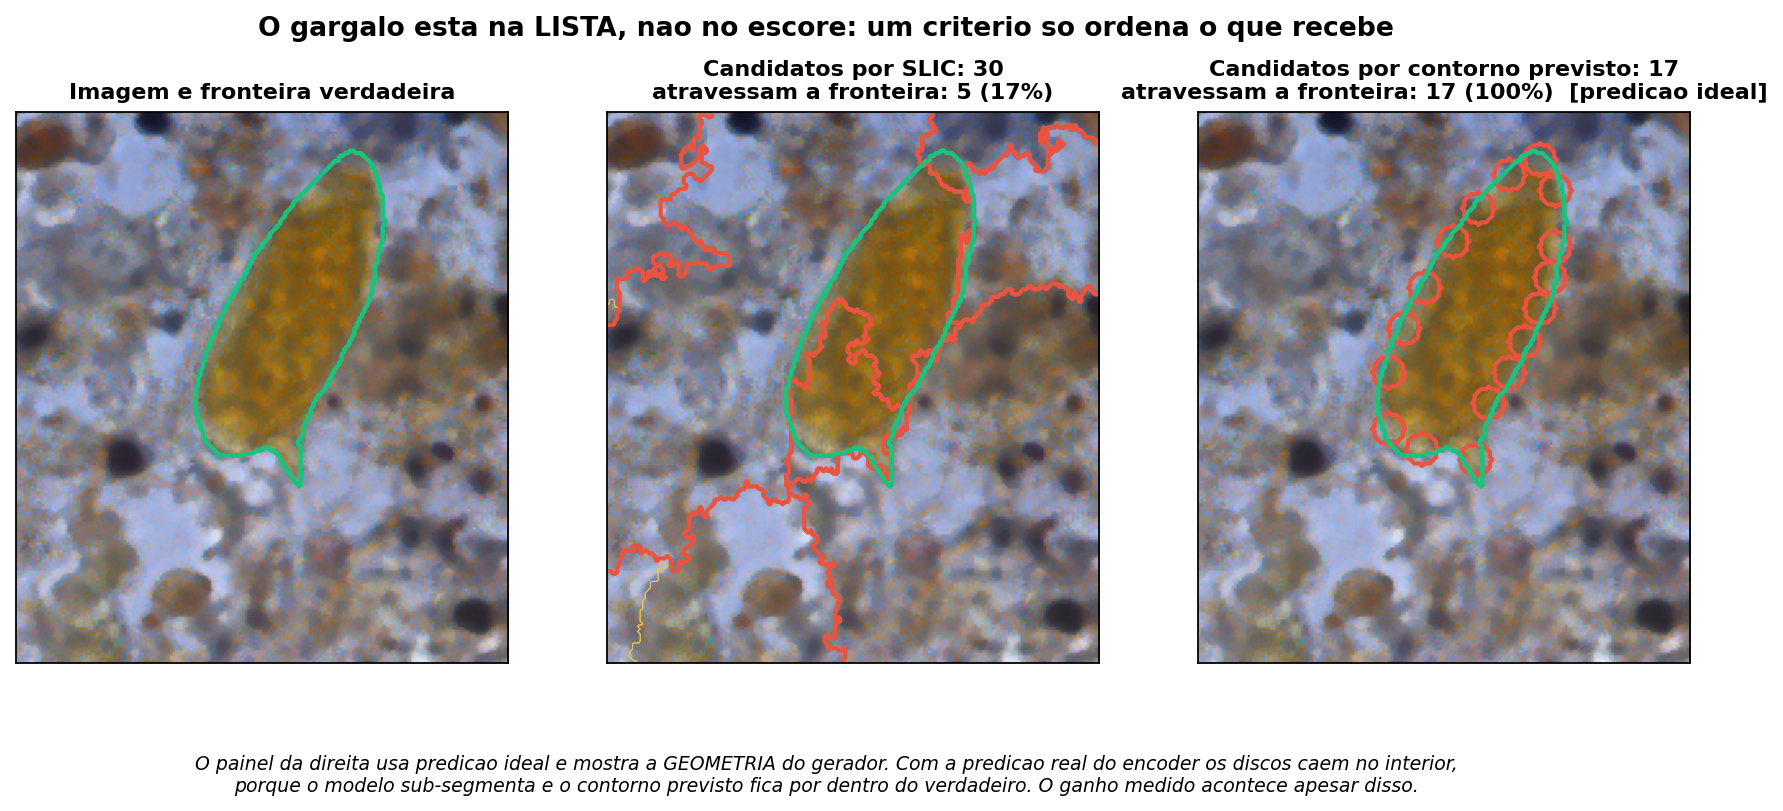
\includegraphics[width=\linewidth]{gerador_candidatos.png}
\caption[O gargalo na geração de candidatos]{Os dois geradores de candidatos sobre a mesma imagem. Em vermelho, os candidatos que atravessam a fronteira verdadeira do objeto. O painel da direita usa predição ideal e ilustra a geometria do gerador proposto; com a predição real do codificador os discos caem no interior, e o ganho medido ocorre apesar disso.}
\label{fig_gargalo}
\end{figure}

A Tabela~\ref{tab_mecanismo} completa o quadro medindo o que \emph{prevê} o ganho de anotar uma região. A entropia da região correlaciona com o ganho no decodificador \texttt{FLIM\_lm} do conjunto de parasitas, com coeficiente de 0,427 e valor p de 0,0001, mas não no \texttt{FLIM\_pb}, onde o coeficiente é de $-0{,}045$ com valor p de 0,6400. O escore não é inútil; ele é dependente do decodificador.

\begin{table}[htb]
\centering
\caption{O que prevê o ganho de anotar uma região.}
\label{tab_mecanismo}
% O que prevê o ganho de anotar uma região — Parasitas, FLIM_lm
% GERADO por flim_al/tabelas.py em 2026-10-06T16:49:57+00:00
% NAO EDITE A MAO: a proxima geracao sobrescreve, e o numero editado deixa de bater com evidencia/execucoes/.
% Proveniencia: ganho_mecanismo_schisto_FLIM_lm_funcional.proveniencia.json
\begin{tabular}{lrrrr}
\hline
variável & $\rho$ de Spearman com $\Delta$ F$\beta$ & IC95\% & n (sementes) & p ($\rho$ $\neq$ 0) \\
\hline
entropia da região & 0.427 & [0.292, 0.562] & 10 & 0.0001 \\
least confidence & 0.427 & [0.292, 0.562] & 10 & 0.0001 \\
fração de foreground & 0.308 & [0.221, 0.395] & 10 & 0.0000 \\
$\Delta$ kernels do encoder & -0.299 & [-0.429, -0.170] & 10 & 0.0005 \\
($\Delta$ F$\beta$ médio ao anotar região de objeto) & -0.0740 & [-0.1661, 0.0181] & 10 & --- \\
($\Delta$ F$\beta$ médio ao anotar região de fundo) & -0.1077 & [-0.1816, -0.0339] & 10 & --- \\
\hline
\end{tabular}

\end{table}

% Nota de ganho_mecanismo_schisto_FLIM_lm_funcional. GERADA por flim_al/tabelas.py.
\footnotesize $\rho$ calculado \textbf{dentro} de cada semente, sobre os candidatos sorteados daquela semente; são os $\rho$ por semente que entram no teste, com n = sementes. Agregar candidatos de sementes diferentes num $\rho$ único trataria observações correlacionadas como independentes. \texttt{entropia da região} é o escore que o Active Learning usa para decidir --- um $\rho$ indistinguível de zero significa que o escore não ordena as regiões por utilidade, e é isso que explicaria todos os resultados negativos das campanhas anteriores. \texttt{$\Delta$ kernels} mede capacidade, não posição: é quantos filtros a mais o encoder extraiu com o marcador extra.
\normalsize


A linha de variação do número de núcleos merece atenção separada. Ela tem correlação \emph{negativa} com o ganho, de $-0{,}299$ com valor p de 0,0005, isto é, acrescentar mais núcleos ao codificador tende a piorar o resultado. Essa linha mede capacidade, não posição, e foi ela que serviu de base ao mecanismo declarado antes da execução da intervenção descrita adiante. Correlação de núcleos com ganho não é, contudo, demonstração de causalidade, e o texto não a trata como tal.

Os critérios de diversidade, avaliados no nível de região pela primeira vez neste trabalho, comportam-se de forma ainda menos favorável. CoreSet localiza o objeto apenas no conjunto de conjuntivite, onde os objetos são grandes, e nos demais seleciona fundo em todas as escolhas, sem qualquer enriquecimento sobre a taxa de base. O medoide nunca localiza o objeto. A explicação é o desequilíbrio do conjunto de candidatos: a diversidade é calculada sobre a distribuição de aparência das regiões, e quando o objeto ocupa cerca de 3\% da imagem ele não participa dessa distribuição de forma relevante. Nos dois conjuntos de objetos pequenos, CoreSet e medoide, que são critérios opostos, produzem a mesma resposta.

\section{Posição ou composição? O controle que separa as duas}

Uma objeção precisa ser respondida antes de atribuir o efeito à posição da anotação. Escolher uma região incerta não escolhe apenas um \emph{lugar}: escolhe junto uma \emph{composição} de classes. Regiões incertas concentram muito mais objeto do que a média, cerca de 73\% contra 16\%, proporção medida antes da execução. Se o ganho viesse de anotar mais objeto, e não de anotar na posição certa, a conclusão do capítulo mudaria.

O experimento que separa as duas coisas fixa o orçamento em pixels anotados por imagem, usa as mesmas imagens em todos os braços, e acrescenta um braço de controle: anotação sorteada, mas com a \emph{mesma proporção} entre objeto e fundo que a seleção por incerteza produz. Se o ganho fosse de composição, esse braço o reproduziria.

\begin{table}[htb]
\centering
\caption{Onde anotar, com orçamento fixo em pixels por imagem.}
\label{tab_onde_marcar}
% Onde anotar, com orçamento fixo em pixels: Fβ e as duas diferenças
% GERADO por flim_al/tabelas.py em 2026-10-08T13:52:40+00:00
% NAO EDITE A MAO: a proxima geracao sobrescreve, e o numero editado deixa de bater com evidencia/execucoes/.
% Proveniencia: onde_marcar.proveniencia.json
\begin{adjustbox}{max width=\linewidth}
\begin{tabular}{lllrrrrrr}
\toprule
braço & px/imagem & decoder & n & F$\beta$ médio & $\Delta$ vs uniforme & p & $\Delta$ vs balanceado & p  \\
\midrule
regiao\_incerteza & 2000 & FLIM\_lm & 5 & 0.247 & -0.215 & 0.022 & -0.256 & 0.013 \\
regiao\_incerteza & 2000 & FLIM\_pb & 5 & 0.476 & -0.167 & 0.019 & 0.209 & 0.051 \\
regiao\_incerteza & 4000 & FLIM\_lm & 5 & 0.055 & -0.283 & 0.022 & -0.054 & 0.263 \\
regiao\_incerteza & 4000 & FLIM\_pb & 5 & 0.488 & -0.142 & 0.023 & 0.305 & 0.037 \\
regiao\_incerteza & 8000 & FLIM\_lm & 5 & 0.000 & -0.011 & 0.264 & 0.000 & 1.000 \\
regiao\_incerteza & 8000 & FLIM\_pb & 5 & 0.410 & -0.189 & 0.129 & 0.239 & 0.121 \\
regiao\_aleatoria & 2000 & FLIM\_lm & 5 & 0.437 & -0.024 & 0.566 & -0.066 & 0.489 \\
regiao\_aleatoria & 2000 & FLIM\_pb & 5 & 0.599 & -0.044 & 0.048 & 0.331 & 0.002 \\
regiao\_aleatoria & 4000 & FLIM\_lm & 5 & 0.387 & 0.049 & 0.412 & 0.278 & 0.037 \\
regiao\_aleatoria & 4000 & FLIM\_pb & 5 & 0.622 & -0.008 & 0.688 & 0.439 & 0.006 \\
regiao\_aleatoria & 8000 & FLIM\_lm & 5 & 0.070 & 0.059 & 0.303 & 0.070 & 0.229 \\
regiao\_aleatoria & 8000 & FLIM\_pb & 5 & 0.602 & 0.003 & 0.974 & 0.431 & 0.003 \\
regiao\_borda & 2000 & FLIM\_lm & 5 & 0.501 & 0.039 & 0.389 & -0.002 & 0.968 \\
regiao\_borda & 2000 & FLIM\_pb & 5 & 0.620 & -0.024 & 0.247 & 0.352 & 0.002 \\
regiao\_borda & 4000 & FLIM\_lm & 5 & 0.391 & 0.052 & 0.490 & 0.281 & 0.003 \\
regiao\_borda & 4000 & FLIM\_pb & 5 & 0.631 & 0.001 & 0.960 & 0.448 & 0.008 \\
regiao\_borda & 8000 & FLIM\_lm & 5 & 0.056 & 0.045 & 0.375 & 0.056 & 0.352 \\
regiao\_borda & 8000 & FLIM\_pb & 5 & 0.477 & -0.122 & 0.402 & 0.306 & 0.122 \\
uniforme\_balanceado & 2000 & FLIM\_lm & 5 & 0.503 & 0.042 & 0.606 & --- & --- \\
uniforme\_balanceado & 2000 & FLIM\_pb & 5 & 0.268 & -0.376 & 0.001 & --- & --- \\
uniforme\_balanceado & 4000 & FLIM\_lm & 5 & 0.109 & -0.229 & 0.111 & --- & --- \\
uniforme\_balanceado & 4000 & FLIM\_pb & 5 & 0.183 & -0.447 & 0.009 & --- & --- \\
uniforme\_balanceado & 8000 & FLIM\_lm & 5 & 0.000 & -0.011 & 0.264 & --- & --- \\
uniforme\_balanceado & 8000 & FLIM\_pb & 5 & 0.171 & -0.428 & 0.008 & --- & --- \\
\bottomrule
\end{tabular}
\end{adjustbox}

\end{table}

% Nota de onde_marcar. GERADA por flim_al/tabelas.py.
\footnotesize Orçamento em \textbf{pixels anotados por imagem}, não em imagens: o que limita o FLIM é a quantidade de pixels marcados --- a mesma imagem rende 54 kernels por camada com traço esparso e 200 com traço denso. Todos os braços gastam exatamente o mesmo número de pixels, nas MESMAS imagens (as do artigo); o que muda é onde eles caem. \texttt{uniforme} é o FLIM de hoje. \texttt{uniforme\_balanceado} tem a mesma proporção objeto/fundo que a incerteza produz, com os pixels sorteados --- é ele que separa *onde se anotou* de *quanto de cada classe se anotou*, porque escolher região incerta escolhe junto muito mais foreground (~73\% contra ~16\%, medido antes de rodar). \texttt{regiao\_borda} usa o gabarito e é teto, não método. Diferenças pareadas por semente; p de t pareado bicaudal. Campanha \texttt{onde\_marcar/k3/teste60/seg300}.
\normalsize


O resultado é desfavorável à seleção por incerteza em todas as seis células, com diferenças contra o braço uniforme entre $-0{,}011$ e $-0{,}283$. E o braço balanceado, que isola a composição, não reproduz o comportamento do braço de incerteza: o que separa os braços é o balanceamento de classe, e não a posição escolhida pelo escore. O braço de borda, que consulta o gabarito e portanto é teto e não método, fica dentro do ruído do uniforme.

A leitura conjunta com a Seção~\ref{sec_custo_al} é a seguinte. Existe margem na posição, e ela é grande. Mas o escore de incerteza, aplicado sobre superpixels, não a captura e ainda introduz um viés de composição que atrapalha. É o terceiro elo do argumento que leva ao gerador.

A Tabela~\ref{tab_regiao_vs_imagem} fecha a comparação por decodificador, e serve de lembrete de que os sete decodificadores de uma mesma célula compartilham o codificador: eles não são observações independentes entre si, e os valores p das suas linhas não se somam.

\begin{table}[htb]
\centering
\caption{Seleção por região contra o controle, por decodificador.}
\label{tab_regiao_vs_imagem}
% Active Learning por região: braços e controle, por decoder
% GERADO por flim_al/tabelas.py em 2026-10-08T14:01:02+00:00
% NAO EDITE A MAO: a proxima geracao sobrescreve, e o numero editado deixa de bater com evidencia/execucoes/.
% Proveniencia: regiao_vs_imagem.proveniencia.json
\begin{tabular}{lrrrrrr}
\toprule
decoder & al (média) & random (média) & n células & $\Delta$ & p & veredito \\
\midrule
decoder\_2 & 0.532 & 0.461 & 9 & 0.036 & 0.5113 & sem suporte \\
decoder\_3 & 0.395 & 0.316 & 9 & 0.033 & 0.6159 & sem suporte \\
decoder\_attention & 0.217 & 0.176 & 9 & 0.091 & 0.1743 & sem suporte \\
hybrid\_decoder & 0.394 & 0.384 & 9 & 0.079 & 0.1107 & sem suporte \\
labeled\_marker & 0.512 & 0.524 & 9 & -0.030 & 0.2452 & sem suporte \\
vanilla\_adaptive\_decoder & 0.429 & 0.413 & 9 & 0.030 & 0.4782 & sem suporte \\
vanilla\_adaptive\_decoder\_wt & 0.195 & 0.170 & 9 & \textbf{0.112} & 0.0471 & suportado \\
\bottomrule
\end{tabular}

\end{table}

% Nota de regiao_vs_imagem. GERADA por flim_al/tabelas.py.
\footnotesize $\Delta$ = al - random, teste \textbf{pareado}, pareado por semente. Só entram células em que os dois braços existem no \textbf{mesmo orçamento} --- o braço do artigo para em 3-4 imagens e o de AL vai a 9, e comparar orçamentos diferentes mediria duas coisas ao mesmo tempo. Negrito só com p < 0,05. Cada linha é um decoder; eles compartilham o encoder dentro de cada célula, então \textbf{não são observações independentes entre si} --- não some os p.
\normalsize


\section{Aprendizado contínuo sem retropropagação}

O esquecimento catastrófico, tal como descrito na Seção \ref{sec_cl}, é atribuído ao deslocamento dos pesos durante o ajuste por gradiente, e os métodos que o combatem atuam sobre esse deslocamento. Como o \ac{FLIM} não possui otimizador, nenhum desses métodos se aplica diretamente. O fenômeno, contudo, existe, e os resultados da seção anterior o quantificam: uma anotação adicional pode reduzir o $F_\beta$ em até meio ponto.

A inspeção do procedimento de estimação dos filtros localiza a origem. Os candidatos a filtro extraídos de todas as imagens e de todos os marcadores são reunidos em um único conjunto, que então é reduzido ao número de canais da camada por um agrupamento. Acrescentar marcadores acrescenta candidatos, o agrupamento é refeito sobre o conjunto ampliado, e os centróides que estavam em uso se deslocam. O banco de filtros é compartilhado por todas as imagens, inclusive as não anotadas, de modo que a perturbação é global e não local.

O mecanismo de retenção proposto no Capítulo \ref{cap_3} interpola o banco: cada centróide novo é ancorado no centróide anterior mais próximo, com um parâmetro de plasticidade que vai de retenção total a reestimação completa. A verificação de corretude confirma as duas extremidades, reproduzindo o comportamento original em um extremo e impedindo a entrada de qualquer direção nova no outro.

A avaliação, porém, não encontrou valor de plasticidade que convertesse o mecanismo em ganho mensurável. O teste primário, declarado antes da execução, comparou plasticidade intermediária contra reestimação completa e não atingiu significância, com sinais inconsistentes entre os tipos de região examinados. A retenção total chegou a parecer vantajosa em uma análise exploratória, mas o resultado não sobreviveu ao aumento do número de repetições nem ao teste em imagens inéditas, e o critério de falseamento declarado no pré-registro foi atingido: a qualidade final sob retenção total é menor, o que contraria a explicação proposta de que congelar o banco evitaria dano sem custo.

\section{Esforço de anotação}

O eixo da segmentação interativa é diferente do $F_\beta$ a orçamento fixo. A métrica usual é o número de cliques necessários para que a qualidade ultrapasse um alvo, com um teto de interações. Um método pode não alterar o $F_\beta$ a orçamento fixo e ainda assim reduzir o esforço de interação.

\begin{table}[htb]
\centering
\caption{Cliques até a qualidade alvo, por plasticidade do banco de filtros.}
\label{tab_noc}
% Cliques até a IoU alvo, por plasticidade do banco de filtros
% GERADO por flim_al/tabelas.py em 2026-10-08T14:01:07+00:00
% NAO EDITE A MAO: a proxima geracao sobrescreve, e o numero editado deixa de bater com evidencia/execucoes/.
% Proveniencia: noc_noc.proveniencia.json
\begin{adjustbox}{max width=\linewidth}
\begin{tabular}{lrrrrrrrrr}
\toprule
dataset & $\alpha$ & n & NoC médio & NoC mediano & taxa de sucesso & IoU final & $\Delta$ NoC vs $\alpha$=1 & p & McNemar \\
\midrule
Parasitas & 0.00 & 38 & 11.03 & 12.0 & 13\% & 0.5267 & -0.53 & 0.1031 & 3/0 (p=0.250) \\
Parasitas & 0.50 & 22 & 11.09 & 12.0 & 14\% & 0.5490 & -0.55 & 0.2876 & 2/0 (p=0.500) \\
Parasitas & 1.00 & 38 & 11.55 & 12.0 & 5\% & 0.5501 & --- & --- & --- \\
BraTS & 0.00 & 40 & 7.42 & 12.0 & 48\% & 0.4096 & -0.35 & 0.5829 & 4/3 (p=1.000) \\
BraTS & 0.50 & 20 & 6.00 & 3.0 & 60\% & 0.5273 & 0.05 & 0.7715 & 1/1 (p=1.000) \\
BraTS & 1.00 & 40 & 7.78 & 12.0 & 45\% & 0.4064 & --- & --- & --- \\
Conjuntivite & 0.00 & 1 & 12.00 & 12.0 & 0\% & 0.0000 & --- & --- & 0/1 (p=1.000) \\
Conjuntivite & 0.50 & 1 & 6.00 & 6.0 & 100\% & 0.7617 & --- & --- & 0/0 (p=1.000) \\
Conjuntivite & 1.00 & 1 & 6.00 & 6.0 & 100\% & 0.7764 & --- & --- & --- \\
\bottomrule
\end{tabular}
\end{adjustbox}

\end{table}

% Nota de noc_noc. GERADA por flim_al/tabelas.py.
\footnotesize NoC@X é o número de cliques até a IoU passar do alvo, com teto de 12; é o eixo de RITM (arXiv:2102.06583) e SimpleClick (arXiv:2210.11006), e \textbf{não} se compara com o NoC publicado deles, que usa outros conjuntos e outra definição de alvo. Imagem que não atinge o alvo entra com o teto, e por isso a \textbf{taxa de sucesso} aparece em toda linha: um braço pode mostrar NoC baixo por desistir mais cedo. \texttt{$\alpha$=1} é o FLIM puro, que refaz o banco de filtros a cada clique; \texttt{$\alpha$=0} congela o banco, e o clique chega ao modelo só pelos rótulos que o decoder \texttt{labeled\_marker} lê. Os testes são \textbf{separados por dataset}: agregar Schisto e BraTS, com 7\% e 30\% de sucesso, inflou um achado exploratório a p=0,0265 que separado não passa de p=0,10. O clique é simulado do ground truth pelo protocolo de Xu et al. (2016), com usuário que acerta sempre, então a tabela mede \textbf{número de interações e não tempo de especialista}.
\normalsize


O comportamento mais informativo dessa avaliação não é o valor médio, e sim a ocorrência de regressão. Em várias execuções o modelo piora ao longo da sequência de cliques: em um caso representativo, doze interações levaram a qualidade de 0,724 para 0,702. O especialista anota repetidamente e o modelo não avança, porque cada anotação nova reestima o banco de filtros e desfaz parte do que havia sido construído.

A proteção do banco não reduziu o número de cliques de forma significativa, e o confirmatório em imagens inéditas falseou tanto a hipótese quanto o mecanismo proposto para ela. A taxa de sucesso é reportada ao lado da contagem de cliques porque imagens que não atingem o alvo entram com o teto, e um braço poderia exibir contagem baixa simplesmente por desistir antes.

\begin{table}[htb]
\centering
\caption{Confirmatório em imagens inéditas.}
\label{tab_noc_conf}
% Cliques até a IoU alvo, por plasticidade do banco de filtros
% GERADO por flim_al/tabelas.py em 2026-10-08T14:01:07+00:00
% NAO EDITE A MAO: a proxima geracao sobrescreve, e o numero editado deixa de bater com evidencia/execucoes/.
% Proveniencia: noc_confirmatorio.proveniencia.json
\begin{adjustbox}{max width=\linewidth}
\begin{tabular}{lrrrrrrrrr}
\toprule
dataset & $\alpha$ & n & NoC médio & NoC mediano & taxa de sucesso & IoU final & $\Delta$ NoC vs $\alpha$=1 & p & McNemar \\
\midrule
Parasitas & 0.00 & 18 & 11.50 & 12.0 & 6\% & 0.5179 & 0.00 & 1.0000 & 0/0 (p=1.000) \\
Parasitas & 1.00 & 18 & 11.50 & 12.0 & 6\% & 0.5646 & --- & --- & --- \\
BraTS & 0.00 & 20 & 9.50 & 12.0 & 30\% & 0.2515 & -0.10 & 0.9138 & 2/2 (p=1.000) \\
BraTS & 1.00 & 20 & 9.60 & 12.0 & 30\% & 0.2770 & --- & --- & --- \\
\bottomrule
\end{tabular}
\end{adjustbox}

\end{table}

% Nota de noc_confirmatorio. GERADA por flim_al/tabelas.py.
\footnotesize NoC@X é o número de cliques até a IoU passar do alvo, com teto de 12; é o eixo de RITM (arXiv:2102.06583) e SimpleClick (arXiv:2210.11006), e \textbf{não} se compara com o NoC publicado deles, que usa outros conjuntos e outra definição de alvo. Imagem que não atinge o alvo entra com o teto, e por isso a \textbf{taxa de sucesso} aparece em toda linha: um braço pode mostrar NoC baixo por desistir mais cedo. \texttt{$\alpha$=1} é o FLIM puro, que refaz o banco de filtros a cada clique; \texttt{$\alpha$=0} congela o banco, e o clique chega ao modelo só pelos rótulos que o decoder \texttt{labeled\_marker} lê. Os testes são \textbf{separados por dataset}: agregar Schisto e BraTS, com 7\% e 30\% de sucesso, inflou um achado exploratório a p=0,0265 que separado não passa de p=0,10. O clique é simulado do ground truth pelo protocolo de Xu et al. (2016), com usuário que acerta sempre, então a tabela mede \textbf{número de interações e não tempo de especialista}.
\normalsize


Duas advertências de leitura acompanham a Tabela~\ref{tab_noc}. A primeira é que as linhas do conjunto de conjuntivite têm $n$ igual a um, e uma única execução não autoriza leitura alguma; elas constam para que a ausência de dado seja visível, e não para serem interpretadas. A segunda é de método, e vale mais que o resultado em si: uma versão anterior desta análise agregava os conjuntos de parasitas e BraTS numa única comparação e obtinha valor p de 0,0265, o que parecia um achado. Separados por conjunto, como manda o protocolo, nenhum dos dois passa de 0,10. A agregação inflava o resultado porque os conjuntos têm taxas de sucesso muito diferentes, de 7\% e 30\%, e misturá-las cria uma diferença que não é do critério.

\section{A intervenção no gerador de candidatos}

As seções anteriores convergem para um diagnóstico. Existe margem considerável na escolha da região. Os critérios de incerteza localizam o objeto mas pousam no interior. Os critérios de diversidade não localizam o objeto. E a anotação que os marcadores dos especialistas mostram ser valiosa, a que atravessa a fronteira, corresponde a uma fração mínima do conjunto de candidatos. Como um critério apenas ordena a lista que recebe, nenhuma escolha de escore poderia resolver a limitação.

A intervenção que decorre desse diagnóstico atua sobre o gerador. Em lugar de segmentar a imagem em superpixels, os candidatos passam a ser discos centrados em pontos do contorno previsto pelo modelo, de modo que atravessam a fronteira por construção. O contorno usado é o previsto, não o do ground truth, e portanto o procedimento é aplicável.

O experimento fixa o critério de seleção em sorteio nos dois braços e mantém o orçamento de anotação idêntico, verificado em mediana de trezentos pixels em ambos. A única diferença entre os braços é a origem da lista de candidatos, o que isola o efeito do gerador.

\begin{table}[htb]
\centering
\caption{Troca do gerador de candidatos, com critério e orçamento fixos.}
\label{tab_gerador}
% Gerador de candidatos: contorno previsto contra superpixel
% GERADO por flim_al/tabelas.py em 2026-10-08T14:01:07+00:00
% NAO EDITE A MAO: a proxima geracao sobrescreve, e o numero editado deixa de bater com evidencia/execucoes/.
% Proveniencia: gerador_contorno.proveniencia.json
\begin{adjustbox}{max width=\linewidth}
\begin{tabular}{lrrrrrrrrrrr}
\toprule
dataset & n & $\Delta$ médio & IC95\% & vitórias & p (t) & p (sinais) & p (perm.) & $\Delta$ pior caso & p  & $\Delta$ dispersão & p   \\
\midrule
Parasitas & 10 & 0.0772 & [0.0393, 0.1151] & 10 de 10 & 0.0013 & 0.0020 & 0.0020 & 0.2153 & 0.0001 & -0.1091 & 0.0000 \\
BraTS & 3 & -0.0089 & [-0.3263, 0.3084] & 1 de 3 & 0.9145 & 1.0000 & 0.7500 & -0.1063 & 0.2703 & 0.0464 & 0.1376 \\
Conjuntivite & 5 & 0.0452 & [-0.0452, 0.1357] & 4 de 5 & 0.2374 & 0.3750 & 0.2500 & 0.1759 & 0.0480 & -0.0577 & 0.1492 \\
\bottomrule
\end{tabular}
\end{adjustbox}

\end{table}

% Nota de gerador_contorno. GERADA por flim_al/tabelas.py.
\footnotesize $\Delta$ é a variação de F$\beta$ na validação ao acrescentar \textbf{uma} anotação, do braço de contorno menos o braço de superpixel. Os dois sorteiam o candidato e gastam os mesmos ~300 px: a \textbf{única} diferença é o gerador da lista, e por isso a comparação isola o gerador e não diz nada sobre qual escore usar. A unidade é a \textbf{semente}; os dois decodificadores de uma semente compartilham o encoder e entram colapsados por média. Pior caso e dispersão foram declarados no pré-registro, com o mecanismo escrito antes de rodar: o candidato de contorno é pequeno e local, acrescenta menos filtros, e o ganho marginal mede correlação negativa entre filtros acrescentados e ganho. O nulo do BraTS é \textbf{previsto}: a arquitetura dele fixa o banco em 8 filtros por camada, os dois braços acrescentam exatamente 24, e o deslocamento que a intervenção evita não pode ocorrer. Semente cuja base degenerou (F$\beta$=0) sai, porque $\Delta$ a partir de zero não pode ser negativo. \textbf{O desfecho primário vem com três testes}: t pareado, teste de sinais e permutação exata de sinais. Com 3 e 5 sementes a normalidade das diferenças não é verificável, e o t sozinho não autorizaria conclusão; onde os três concordam, como no conjunto de parasitas, a conclusão não depende da suposição. \textbf{ATENÇÃO ao pior caso da conjuntivite}: o valor de 0,0480 é bruto e \textbf{não sobrevive} à análise de sensibilidade que casa o número de candidatos entre os braços, na qual passa a 0,1032. O gerador de contorno entregou UM único candidato naquela semente, e mínimo de um sorteio contra mínimo de oito não é comparação. Esse desfecho \textbf{não deve ser lido como significativo}.
\normalsize


No conjunto de parasitas o efeito é claro: ganho médio de 0,0772 de $F_\beta$, com intervalo de confiança entre 0,0393 e 0,1151, valor p de 0,0013, e vantagem em todas as dez repetições. O resultado sobrevive à correção de Benjamini-Hochberg aplicada sobre os três conjuntos de dados. Os dois desfechos secundários, declarados no pré-registro com o mecanismo escrito antes da execução, acompanham: o pior caso melhora 0,2153 e a dispersão entre candidatos cai 0,1091.

O comportamento nos outros dois conjuntos merece atenção. Na conjuntivite o efeito vai na mesma direção, com vantagem em quatro das cinco repetições, mas sem significância no desfecho primário. No BraTS o efeito desaparece, e esse resultado nulo é previsto pelo mecanismo: a arquitetura empregada nesse conjunto fixa o banco em oito filtros por camada, de modo que ambos os braços acrescentam exatamente o mesmo número de filtros e o deslocamento que a intervenção evita não pode ocorrer. O conjunto funciona, assim, como controle do mecanismo.

Duas limitações do gerador foram medidas e devem acompanhar qualquer leitura do resultado. A primeira é que ele exige uma predição não trivial: quando a máscara prevista é vazia ou cobre a imagem inteira, não há contorno e o conjunto de candidatos fica vazio, enquanto o gerador por superpixels funciona em qualquer situação. A segunda é que os candidatos gerados apresentam fração de objeto próxima de um, isto é, caem no interior do objeto verdadeiro e não sobre sua fronteira, porque o modelo subsegmenta e o contorno previsto se situa dentro do contorno real. O ganho ocorre apesar disso, o que sugere que parte do efeito decorre de o candidato ser pequeno e localizado, acrescentando menos filtros ao banco, e não apenas de sua posição. Separar essas duas contribuições exige um experimento adicional, discutido no Capítulo \ref{cap_5}.

\subsection{Análise de sensibilidade dos desfechos secundários}
\label{sec_sensibilidade}

Uma terceira limitação apareceu na conferência dos dados e afeta a leitura dos secundários, não do desfecho primário. O desenho declarou oito candidatos por braço, mas o gerador de contorno entregou menos em três sementes: três no conjunto de parasitas, três no BraTS e \emph{uma} na conjuntivite. O gerador por superpixels entregou oito em todas.

A consequência não é a mesma para os três desfechos. A média é estimador não viesado da média do braço qualquer que seja o número de candidatos, de modo que o desfecho primário não se move. Mas o desfecho de pior caso é um \emph{mínimo}, e o mínimo de oito sorteios é, por construção, mais extremo que o mínimo de um, mesmo que a distribuição subjacente seja idêntica. O viés empurra na direção que a tabela reporta, o que obriga a medi-lo.

Refazendo o teste com o braço de superpixels subamostrado ao mesmo número de candidatos, sem reposição, com duas mil repetições e o mesmo teste pareado por semente, obtém-se o seguinte. No conjunto de parasitas o pior caso passa de 0,2153 para 0,2085, com valor p de 0,0002, e a dispersão passa de $-0{,}1091$ para $-0{,}1078$, com valor p abaixo de 0,0001: ambos sobrevivem, e o efeito não era artefato do número de candidatos. Na conjuntivite, porém, o pior caso passa de 0,1759 com valor p de 0,0480 para 0,1369 com valor p de 0,1032, isto é, \textbf{cruza o limiar e deixa de ser significativo}. A semente responsável entregou um único candidato de contorno, e mínimo de um sorteio contra mínimo de oito não é comparação.

O desfecho secundário de pior caso na conjuntivite não é, portanto, apresentado como significativo nesta dissertação. Esta análise é de sensibilidade sobre um desfecho pré-registrado, e não um desfecho novo.

\subsection{O critério sobre a lista corrigida}

A intervenção acima troca o gerador mantendo o escore fixo em sorteio, de propósito, para isolar uma coisa de cada vez. Resta a pergunta complementar: uma vez corrigida a lista, o escore volta a ter utilidade?

Uma campanha adicional no conjunto de parasitas, com dez sementes completas, indica que sim, e os dois efeitos se somam de forma quase exata. Aplicar o critério de entropia sobre candidatos de contorno rende 0,0262 de $F_\beta$ sobre sortear dentro da mesma lista, com vantagem em nove das dez sementes e valor p de 0,0185. A troca do gerador isolada rende os 0,0772 já relatados. E o efeito combinado, critério sobre contorno contra sorteio sobre superpixels, rende 0,1033, com vantagem nas dez sementes e valor p de 0,0002. A soma das partes, 0,1034, coincide com o efeito total medido.

A aditividade é coerente com o diagnóstico: o gerador resolve \emph{o que está na lista} e o escore resolve \emph{qual item da lista}, e são operações sobre dimensões distintas do problema.

Duas ressalvas limitam o alcance desse resultado. Ele vem de um único conjunto de dados, e \textbf{não houve pré-registro para estas comparações}, de modo que elas são exploratórias e servem para orientar o próximo passo, não para afirmar. Registra-se também que a terceira linha dessa campanha reproduz exatamente o ganho de 0,0772 já publicado, com o mesmo valor p e as mesmas dez vitórias, o que serve de verificação interna: um cálculo novo, sobre uma campanha nova, devolveu o número anterior.

\section{Comparação com redes treinadas por retropropagação}

Para situar a ordem de grandeza dos valores acima, cinco redes de segmentação treinadas por retropropagação foram avaliadas nos dois conjuntos de maior porte, com três partições cada. No conjunto de parasitas os valores de $F_\beta$ ficam entre 0,3763 e 0,4450, e no BraTS entre 0,7421 e 0,8511.

A comparação direta com os números do \ac{FLIM} apresentados neste capítulo \textbf{não é válida} e não é feita aqui, por três razões que convém enunciar em vez de contornar. As redes por retropropagação foram treinadas com o conjunto de treino completo e anotação densa, enquanto o \ac{FLIM} opera com três a cinco imagens e traços esparsos, de modo que o orçamento de anotação difere por ordens de grandeza. Os protocolos de avaliação e as partições não coincidem. E, principalmente, esses resultados \textbf{não estão no registro canônico de execuções} que sustenta todas as demais tabelas deste capítulo, tendo proveniência mais fraca que o restante.

O que eles autorizam é apenas uma observação de contexto: no conjunto de parasitas, o patamar alcançado por redes com supervisão densa é da ordem de 0,44, enquanto o \ac{FLIM} com três marcadores reais atinge 0,744 no decodificador \texttt{FLIM\_lm} sob o protocolo de avaliação adotado aqui. Os dois números medem coisas diferentes e a diferença de protocolo é suficiente para explicar a distância; o que não se sustenta é a suposição de que supervisão densa seja condição necessária para desempenho utilizável neste domínio.

\section{Resultados de natureza metodológica}

Três resultados não dizem respeito ao desempenho dos métodos, mas à validade das medições, e por isso são relatados separadamente.

\subsection{Reprodutibilidade do treinamento}

O treinamento do codificador não era reprodutível entre execuções. Duas chamadas idênticas, com os mesmos arquivos de marcadores e no mesmo processo, produziam pesos diferentes quando o número de candidatos a filtro ultrapassava o limite da arquitetura: a diferença máxima observada nos pesos da segunda camada foi de 0,134. Abaixo desse limite o procedimento devolve os próprios candidatos sem agrupá-los, e por isso é estável; acima dele o agrupamento precisa escolher entre muitos candidatos, e a ordem de redução das somas em bibliotecas de álgebra linear com múltiplas linhas de execução altera o resultado no último dígito, o que basta para o agrupamento convergir para outra configuração. O efeito se amplifica entre camadas, já que cada camada recebe como entrada as ativações da anterior.

Fixando as bibliotecas em uma única linha de execução, a diferença passa a ser exatamente zero nos dois regimes. Todas as campanhas posteriores a essa descoberta foram executadas sob essa restrição.

\subsection{Defeitos que invalidaram medições anteriores}

Três defeitos de implementação foram encontrados e corrigidos, e os números produzidos antes das correções não são válidos. O procedimento de extração de atributos para os critérios de diversidade assumia imagens de três bandas, o que impedia sua execução no conjunto BraTS, de banda única. A leitura de imagens assumia extensão fixa, o que impedia a execução no conjunto de conjuntivite. E o filtro de área do pós-processamento estava configurado com a faixa adequada ao conjunto de parasitas, cujos objetos são pequenos, o que eliminava toda componente prevista nas imagens de conjuntivite: nenhum dos objetos examinados cabia na faixa, e o $F_\beta$ mediano passou de 0,024 para 0,594 após a correção.

Esse último caso tem interesse além do defeito pontual. Ele indica que os parâmetros de pós-processamento publicados não transferem entre domínios, e que aplicá-los sem reavaliação pode produzir resultados sem relação com o método avaliado.

\subsection{Falsos positivos capturados pelo protocolo}

O protocolo de pré-registro, descrito no Capítulo \ref{cap_3}, capturou quatro resultados que não se sustentaram. Dois deles haviam atingido significância em análises exploratórias e foram submetidos a confirmatórios com repetições inéditas: um apresentava valor p de 0,0016 e passou a 0,586, outro apresentava 0,082 e passou a 0,567. Um terceiro desapareceu quando o número de repetições foi completado, com o valor p passando de 0,0265 para 0,1385. O quarto foi falseado não apenas na hipótese como no mecanismo proposto, pelo critério declarado antes da execução.

\begin{table}[htb]
\centering
\caption{Composição do registro de execuções.}
\label{tab_proveniencia}
% Proveniência disponível por família de experimento
% GERADO por flim_al/tabelas.py em 2026-10-08T14:01:07+00:00
% NAO EDITE A MAO: a proxima geracao sobrescreve, e o numero editado deixa de bater com evidencia/execucoes/.
% Proveniencia: proveniencia_registro.proveniencia.json
\begin{tabular}{lrrr}
\toprule
família & execuções & sem seed & sem commit \\
\midrule
ganho\_marginal & 2448 & 0\% & 0\% \\
al\_corrected\_results & 2316 & 42\% & 100\% \\
tabela\_k\_por\_modelo & 1840 & 0\% & 0\% \\
final\_comparison\_v3 & 1029 & 4\% & 100\% \\
benchmark\_conjunctiva & 588 & 68\% & 100\% \\
sel\_cs\_grande & 540 & 0\% & 100\% \\
al\_backprop\_results & 492 & 20\% & 100\% \\
paper\_selection\_pac2 & 432 & 0\% & 100\% \\
paper\_selection\_POOL\_COM\_VAZAMENTO & 360 & 0\% & 100\% \\
paper\_selection\_v2 & 324 & 0\% & 100\% \\
paper\_selection\_v3 & 324 & 0\% & 100\% \\
paper\_selection\_rand & 321 & 0\% & 100\% \\
densidade & 262 & 0\% & 0\% \\
cl\_plasticidade & 254 & 0\% & 0\% \\
sel\_degen & 216 & 0\% & 100\% \\
sel\_medoide & 216 & 0\% & 100\% \\
sel\_proposto & 216 & 0\% & 100\% \\
final\_comparison\_v2 & 210 & 10\% & 100\% \\
il\_noc & 207 & 0\% & 0\% \\
clique & 183 & 0\% & 0\% \\
paper\_selection\_coreset & 162 & 0\% & 100\% \\
onde\_marcar & 150 & 0\% & 0\% \\
final\_comparison & 147 & 57\% & 100\% \\
al\_encoder\_results\_acq\_comparison & 144 & 44\% & 100\% \\
orcamento & 144 & 100\% & 100\% \\
artigo\_vs\_regiao & 130 & 0\% & 0\% \\
al\_curve & 84 & 100\% & 100\% \\
brats & 84 & 25\% & 100\% \\
al\_encoder\_results & 70 & 70\% & 100\% \\
al\_encoder\_results\_dt & 62 & 47\% & 100\% \\
paper\_selection\_brats & 54 & 0\% & 100\% \\
paper\_selection\_uB\_POOL\_COM\_VAZAMENTO & 54 & 0\% & 100\% \\
al\_bald\_results & 48 & 44\% & 100\% \\
al\_flim\_curve & 42 & 100\% & 100\% \\
curva & 24 & 100\% & 100\% \\
al\_region\_results & 16 & 44\% & 100\% \\
\bottomrule
\end{tabular}

\end{table}

% Nota de proveniencia_registro. GERADA por flim_al/tabelas.py.
\footnotesize Diagnóstico, não resultado. Linha com 100\% sem seed não sustenta afirmação sobre variância entre execuções.
\normalsize


\section{Síntese}

Os resultados sustentam a seguinte leitura, em quatro elos, cada um medido.

\textbf{Primeiro, a seleção de imagem não é a alavanca.} Nenhum critério de \ac{AL} apresenta superioridade sobre a escolha aleatória que sobreviva à correção para múltiplas comparações, e o procedimento supervisionado do trabalho de referência, que lê o gabarito de todo o conjunto, também não se destaca. Isso não é demonstração de equivalência: é ausência de evidência de superioridade nas condições avaliadas.

\textbf{Segundo, a posição da anotação é.} Com orçamento de pixels fixo e nas mesmas imagens, a melhor região examinada supera a sorteada por 0,1351 a 0,3089 de $F_\beta$, nas seis células, e a pior fica 0,2075 a 0,4954 abaixo. O prêmio e o risco são da mesma ordem, o que significa que anotar mais não é, por si, melhorar.

\textbf{Terceiro, os critérios capturam parte dessa margem, e a parte que escapa é o custo do método.} A lacuna entre o teto e o que o critério entrega vai de 0,0839 a 0,2667 e é significativa em quatro das seis células. O desempenho do escore depende do decodificador e do domínio: há uma célula em que ele captura 84\% da margem e outra em que captura praticamente nada.

\textbf{Quarto, o gargalo está na lista e não no escore.} Regiões que atravessam a fronteira do objeto, que são as que a comparação com os marcadores reais mostra terem valor, representam de 2\% a 12\% dos candidatos produzidos por superpixels. Como um critério apenas ordena a lista que recebe, nenhuma escolha de escore resolveria isso. A intervenção derivada desse diagnóstico, que troca o gerador mantendo escore e orçamento fixos, produz ganho de 0,0772 de $F_\beta$ no conjunto de parasitas, em dez de dez repetições, sobrevivendo à correção; o resultado nulo no BraTS foi previsto pelo mecanismo antes da execução e funciona como controle dele.

A razão estrutural que percorre os quatro elos é a mesma: no \ac{FLIM}, a anotação adicional \emph{reestima} o extrator de atributos em vez de refiná-lo, e o banco de filtros é compartilhado por todas as imagens, de modo que o acréscimo é uma intervenção global e de risco. O Capítulo \ref{cap_5} discute o que esses resultados autorizam afirmar e o que permanece em aberto.

\chapter{Conclusão}\label{cap_5}

Esta dissertação investigou se estratégias de aprendizado ativo e contínuo transferem para o \ac{FLIM}, um modelo cujos filtros são estimados diretamente de marcadores desenhados pelo especialista, sem retropropagação. A pergunta surge de uma propriedade do trabalho de referência reproduzido aqui: a seleção das poucas imagens a anotar depende do ground truth de todo o conjunto disponível, o que os próprios autores declaram. Como essa dependência contraria a situação que motiva o método, convinha verificar quanto do benefício se recupera com critérios que dispensam a anotação prévia.

\section{Respostas às questões de pesquisa}

A resposta direta é que os critérios conhecidos não transferem, e a investigação permitiu descrever por quê com alguma precisão.

Na seleção de imagens, nenhum critério avaliado apresentou superioridade sobre a escolha aleatória que sobrevivesse à correção para múltiplas comparações. O resultado se manteve em três conjuntos de dados, quatro orçamentos de anotação e sete decodificadores. O oracle, que lê o ground truth e representa o teto do procedimento do trabalho de referência, também não se destacou de forma consistente.

Na seleção de regiões, a situação é mais informativa. Existe margem considerável a ser capturada, entre 0,1351 e 0,3089 de $F_\beta$ separando a melhor região examinada da região sorteada, com significância nas seis combinações de conjunto de dados e decodificador. É esse o valor do clique no lugar certo, e é a razão de a pergunta sobre posição de anotação valer a pena. A simetria do risco reforça o ponto: uma anotação adicional mal posicionada custa entre 0,2075 e 0,4954, de modo que, no \ac{FLIM}, anotar mais não é por si melhorar.

Os critérios capturam parte dessa margem, e a parte que escapa é o resultado quantitativo central deste trabalho: a lacuna entre o teto e o que o critério entrega vai de 0,0839 a 0,2667 e é significativa em quatro das seis células. Essa lacuna é o custo do \ac{AL} no \ac{FLIM}, no sentido preciso de ser o que se deixa na mesa porque o critério erra o lugar do clique. Convém registrar que o desempenho do escore não é uniforme: há uma célula, o \textit{least confidence} no BraTS com o decodificador \texttt{FLIM\_lm}, em que ele captura 84\% da margem com valor p de 0,0012, e outras em que não captura praticamente nada. A conclusão defensável não é que os critérios de incerteza sejam inúteis, e sim que o seu desempenho depende do decodificador e do domínio.

A medição do comportamento deles mostra duas razões distintas para a lacuna. Os critérios de incerteza localizam o objeto com enriquecimento expressivo sobre a taxa de base, mas pousam no interior em vez da fronteira. Os critérios de diversidade, avaliados no nível de região pela primeira vez neste trabalho, não localizam o objeto quando ele ocupa pequena fração da imagem, porque a distribuição de aparência sobre a qual a diversidade é calculada é dominada pelo fundo.

A razão mais consequente, contudo, não está nos critérios. A comparação com os marcadores reais dos especialistas mostra que afastar o clique da posição que eles escolheram, mantendo imagens, número de cliques e traço de fundo idênticos, custa entre 0,075 e 0,182 de $F_\beta$, com significância nas sete linhas avaliadas. E regiões que atravessam a fronteira do objeto representam de 2\% a 12\% do conjunto de candidatos gerado por superpixels. Como um critério apenas ordena a lista que recebe, nenhuma escolha de escore resolveria essa limitação.

Quanto ao aprendizado contínuo, o fenômeno do esquecimento catastrófico existe no \ac{FLIM} e assume forma própria. Sem otimizador, não há deslocamento de pesos por gradiente, e os três grupos de métodos consolidados na literatura, que atuam sobre esse deslocamento, não se aplicam. O que ocorre é que a anotação adicional amplia o conjunto de candidatos a filtro, o agrupamento que os reduz ao número de canais é refeito, e os filtros em uso se deslocam. Como o banco é compartilhado por todas as imagens, a perturbação é global. O mecanismo de retenção proposto resolve o problema que se propõe a resolver, verificado por teste, mas não se converteu em ganho mensurável em nenhum dos regimes avaliados, e a hipótese de que a retenção total preservaria qualidade foi falseada pelo critério declarado antes da execução.

\section{Contribuições}

A principal contribuição é a caracterização do motivo pelo qual as técnicas não transferem, acompanhada da medição de cada elo do argumento. Diferentemente de um relato de que a combinação não funciona, o trabalho localiza o mecanismo no procedimento de estimação dos filtros, mede a magnitude do dano que uma anotação mal posicionada causa, e identifica onde está o gargalo.

A segunda contribuição decorre da primeira. Se o gargalo está na geração dos candidatos e não na sua pontuação, a intervenção pertinente é trocar o gerador. Substituindo superpixels por discos centrados no contorno previsto pelo modelo, com critério de seleção e orçamento de anotação mantidos fixos, o ganho de uma anotação adicional aumentou 0,0772 de $F_\beta$ no conjunto de parasitas, com intervalo de confiança entre 0,0393 e 0,1151 e vantagem em todas as dez repetições, resultado que sobrevive à correção para múltiplas comparações sobre os três conjuntos. O comportamento nos demais conjuntos é compatível com o mecanismo: no BraTS, cuja arquitetura fixa o banco em oito filtros por camada, ambos os braços acrescentam o mesmo número de filtros e o efeito desaparece, de modo que esse conjunto funciona como controle.

A terceira contribuição é de natureza metodológica e tem alcance além deste trabalho. O treinamento do codificador não era reprodutível entre execuções quando o número de candidatos ultrapassava o limite da arquitetura, com divergência de até 0,134 nos pesos, e a causa foi localizada na interação entre o agrupamento e a ordem de redução em bibliotecas de álgebra linear com múltiplas linhas de execução. Além disso, verificou-se que os parâmetros de pós-processamento publicados não transferem entre domínios: a faixa de área adequada ao conjunto de parasitas elimina toda componente prevista no conjunto de conjuntivite, e corrigi-la elevou o $F_\beta$ mediano de 0,024 para 0,594.

Por fim, a plataforma interativa desenvolvida integra os três componentes em um fluxo único, no qual o aprendizado ativo propõe a região, o especialista a rotula, e o parâmetro de plasticidade do banco de filtros pode ser alterado entre interações. Ela permite observar o fenômeno descrito neste trabalho em tempo real, incluindo o caso em que sucessivas anotações não melhoram o modelo.

\section{Limitações}

Os resultados estão sujeitos a limitações que convém enunciar sem atenuação.

A anotação é simulada a partir do ground truth. Nenhum resultado deste trabalho autoriza afirmações sobre redução de tempo de especialista, que exigiriam avaliação com pessoas. No experimento de esforço interativo, o usuário simulado acerta sempre, o que constitui um limite superior otimista para qualquer sistema real.

A avaliação não emprega o delineamento por árvores dinâmicas usado no trabalho de referência, por indisponibilidade do executável na plataforma utilizada. Os valores reproduzidos, portanto, não são diretamente comparáveis aos publicados.

O ganho do gerador de contorno é significativo em um dos três conjuntos de dados. No conjunto de conjuntivite o efeito vai na mesma direção sem atingir significância, e no BraTS é nulo por razão estrutural identificada. Trata-se do primeiro teste de uma intervenção derivada dos próprios dados do projeto, o que pede replicação independente antes de generalização.

A comparação que isola o gerador fixa o critério de seleção em sorteio nos dois braços, de propósito, para medir uma coisa de cada vez. Uma campanha adicional, exploratória e sem pré-registro, indica que o escore volta a agregar sobre a lista corrigida, com os dois efeitos somando-se de forma quase exata, mas esse resultado vem de um único conjunto de dados e não autoriza afirmação.

O gerador de contorno pode entregar \emph{menos} candidatos do que os pedidos quando o contorno predito é curto, e não apenas zero quando a predição é degenerada. Isso ocorreu em três sementes das campanhas, e tem consequência sobre os desfechos secundários, que são estatísticas de extremo e de dispersão: ao casar o número de candidatos entre os braços, o pior caso no conjunto de parasitas sobrevive, mas o da conjuntivite deixa de ser significativo e não é apresentado como tal nesta dissertação.

Os cinco modelos treinados por retropropagação usados como referência de contexto não constam do registro canônico de execuções que sustenta as demais tabelas, tendo proveniência mais fraca. Eles situam ordem de grandeza e não entram em comparação direta.

O teto medido na seleção de região é um máximo sobre os candidatos examinados, e não um teto absoluto, já que apenas parte dos superpixels de cada imagem foi avaliada. O valor deve ser lido como estimativa conservadora da margem disponível.

As repetições de cada campanha compartilham a partição e o conjunto de validação, variando as imagens de treino e os traços. Os intervalos de confiança descrevem a variação sob sorteio das imagens de treino naquele conjunto de validação, e não generalizam para o conjunto de dados como um todo.

Por fim, não existe neste trabalho um controle direto que isole borda de interior com imagens, orçamento e procedimento idênticos. A comparação disponível opõe a anotação dos especialistas, que recai próxima à borda, a cliques uniformes no interior do objeto, que incluem posições próximas à fronteira. O contraste real é provavelmente maior que o medido, mas isso é inferência e não medição.

\section{Trabalhos futuros}

Os resultados sugerem cinco continuações, ordenadas pelo que cada uma esclareceria.

A primeira separa duas explicações que o experimento do gerador deixa confundidas. Os candidatos de contorno são, ao mesmo tempo, mais bem posicionados e menores, e acrescentam menos filtros ao banco. Como a correlação entre filtros acrescentados e ganho é negativa, parte do efeito pode decorrer do tamanho e não da posição. Um experimento que variasse as duas propriedades independentemente, comparando discos de contorno com discos de mesmo tamanho posicionados no interior, resolveria a questão.

A segunda é a ablação da capacidade do banco de filtros. A hipótese de que o dano decorre do deslocamento dos centróides prevê que ele deve crescer conforme a razão entre candidatos e canais disponíveis aumenta. Variar o número de canais no mesmo conjunto de dados, com os mesmos marcadores, testaria essa previsão de forma direta, desde que se verifique que o procedimento permanece válido quando o número de filtros deixa de ser consequência dos padrões disponíveis.

A terceira trata da subsegmentação. Os candidatos gerados sobre o contorno previsto caem no interior do objeto verdadeiro porque o contorno previsto se situa dentro do real. Uma correção que compensasse esse viés poderia aproximar os candidatos da fronteira, mas exigiria justificar a magnitude da correção por evidência independente, e não por ajuste contra a métrica avaliada.

A quarta é o controle direto de borda contra interior, ausente neste trabalho, com imagens, orçamento e procedimento idênticos nos dois braços.

A quinta é a avaliação com especialistas humanos. Todas as conclusões sobre esforço de anotação apoiam-se em usuário simulado, e a região que o modelo considera incerta pode ser também mais difícil de rotular para uma pessoa, o que reduziria o benefício observado em simulação.

\section{Considerações finais}

O percurso desta investigação ilustra uma dificuldade recorrente em pesquisa aplicada: a de distinguir um resultado de um artefato. Quatro achados que haviam atingido significância em análises exploratórias não se sustentaram quando submetidos a repetições inéditas ou quando o número de repetições foi completado, e um deles foi falseado não apenas na hipótese como no mecanismo que lhe fora atribuído. O protocolo de pré-registro, com hipótese, desfecho primário e critério de falseamento declarados antes da execução, foi o que permitiu identificá-los.

Esse aspecto não é acessório ao resultado. Em um espaço de busca com muitos critérios, muitos conjuntos de dados e muitos orçamentos, encontrar uma combinação que pareça funcionar é quase certo mesmo quando nada funciona. O que distingue um achado de um acidente é ter declarado, antes de olhar, o que contaria como evidência.


\bookmarksetup{startatroot}% 
% ---

% ---
% Conclusão
% ---

% ----------------------------------------------------------
% ELEMENTOS PÓS-TEXTUAIS
% ----------------------------------------------------------
\postextual

% ----------------------------------------------------------
% Referências bibliográficas
% ----------------------------------------------------------
\bibliography{referencias/referencias}

\end{document}


